% docx2tex --- ``Garbage In, Garbage Out'' 
% 
% docx2tex is Open Source and  
% you can download it on GitHub: 
% https://github.com/transpect/docx2tex 
%  
\documentclass{scrbook}  
\usepackage{graphicx} 
\usepackage{hyperref} 
\usepackage{multirow} 
\usepackage{amsmath} 
\usepackage{amssymb} 
\usepackage{amsfonts} 
\usepackage{wasysym} 
\usepackage{isomath} 
\usepackage{upgreek} 
\usepackage{enumerate} 
\usepackage{morefloats}
\usepackage[ngerman]{babel} 
  
\begin{document}

\includegraphics[width=1\textwidth]{gc-core-rules.docx.tmp/word/media/image1.png}

 GreenCloaks Core	Rules

Version 2.5

Released March 2015

\tableofcontents

Green Cloaks Core Rules {\textcopyright} \textit{Trinity Games} 2015

\chapter{Introduction}

\textbf{Welcome to} \textbf{\textit{Green Cloaks}}

The \textit{Green Cloaks} game takes place within the Segovax Cluster, a significant star cluster far from Terra. Five systems here form the bastion of humanity on this isolated fringe of the galaxy. The cluster is a place ringed in beauty, mystery and legend. It is here the fabric of reality is said to flex with the ebb and flow of time, and it is amongst these very stars that you will decide the future of humankind and its allies.

The human race, united under the banner of the Terran Sovereignty, has spread throughout the galaxy in the last 3000 years, colonising and terraforming planets to make them habitable, an expansion made necessary following a cataclysmic nuclear war and 1000 years of ruin. They share the galaxy with a multitude of other races, and informal alliances have been formed between them. Some of these races

have the knowledge of technology far more advanced than others; some are pacifist in nature; others seem primitive but with a complex and deep sense of loyalty. Together they fight against their mutual enemies

to push back the front lines from their homeworlds, and in some cases reclaim their lost planets from the aggressor.

Terran technology has advanced little in this time, as humans concentrated instead on spreading out to the stars lest humanity come close to extinction again, and the tech of the enemy is often superior. New tools must be designed, new weapons engineered to allow for the chance of victory.

You are enrolled in one of four regiments that make up a special taskforce in the Terran Sovereignty Army known as the Green Cloaks, named for their ballistic weave cloaks, the only armour that can be mass- produced with the limited resources available at this time of war. Your missions are varied and dangerous, pitted against the enemies of the human race and its allies.

Join the regiments of the Green Cloaks as they seek to defend the Sovereignty, defeat their enemies and overcome the challenges of a seemingly hostile universe.

\textit{Green Cloaks} is a NERF-based LARP system founded in 2012 by Enys Coggles with collaborator Adam Wojcik. As a grassroots system it is perfect for individuals new to LARP wanting to try out the hobby, but it has plenty to also grab the interest of more experienced LARPers and roleplayers. The system offers a friendly atmosphere and an enthralling plot for people of all levels of LARP experience.

With a friendly game team always willing and able to help enhance your experience and gameplay, our aim is to ensure that you are encouraged in your LARP experience, and to bring new people to the hobby.

Thank you for your interest, and we at \textit{Green Cloaks} look forward to seeing you at our events.

The \textit{Green Cloaks} rulebook is divided into five parts, and not all of them are applicable to every character

you may wish to play.

The \textbf{\textit{Introduction}} gives you an explanation of what to expect at a LARP game, and features the timeline of events leading up to very recent years. This timeline is useful to give you a context in which to play the game, and a feel for the world in which \textit{Green Cloaks} is set.

\textbf{\textit{Part 1}} is all about playing the game. This includes rules to keep everybody safe and acceptable behaviour, which we hope you will read at least once. However, this is also the place to look for some of the essential rules of the game, including the \textbf{calls} the game uses to indicate certain effects, how \textbf{dying}, \textbf{healing}

and \textbf{stabilisation} works, how your character's \textbf{hits} work, and what an \textbf{encounter} is. Many of the uses of skills in \textit{Green Cloaks} rely on this concept of an encounter, so you must read this section to gain an understanding of it. Please note that although \textit{Chapter 8: Calls} seems to list a lot of calls, they include all Omega ability calls (analogous to spell effects in other systems), which in many other LARP systems and RPG games would be listed separately. They are listed together so that you have a single section to reference rather than two.

\textbf{\textit{Part 2}} guides you through \textbf{character creation}, including lots of information about the different \textbf{races} you can play, the \textbf{planets} your character could come from, and the \textbf{regiments} you can join. This is also the place where you will find information on all the \textbf{skills} you can use, \textbf{classes} you can play, and \textbf{equipment} your character might use. This is pretty essential reading for any player, and no doubt you'll refer to it frequently as you experience more of the \textit{Green Cloaks} system.

\textbf{\textit{Part 3}} is where you can find information about four very specific areas of the game: \textbf{Engineering}, \textbf{Pharmacology}, \textbf{Thaumaturgy} and the \textbf{Omega plane}. If you don't want to play somebody with the Engineering or Pharmacology skills, or don't want to play a character that uses Omega powers, you can ignore this section (though you might find it interesting to know how this works).

Finally, the \textbf{\textit{Appendices}} are useful resources, filled with handy skill times and costs charts for ease of reference, diagrams, sample character builds, and crafting lists. You'll also find a guide to blaster safety provided by \textit{Blastersmiths UK}, a guide to the categories that currently available blasters fall into, and copies of the character sheet and disclaimer you'll need to fill out at events.

LARP (Live Action Roleplay), is an immersive game that can be described as a mixture of collaborative storytelling, creative world-building, outdoor activity, and sport. It's a game for everyone, regardless of background, profession, or gender: the only requirement is a little bit of imagination (which everybody has). In a LARP game you create a character that lives in, and interacts with, a persistent world that is created and populated by the game organizers, referees and crew, in which there are other players doing exactly the same. Your character will have a personality, skills and abilities, and these will help you decide how to react to this world and what happens in it. You can create almost any kind of character, and that character has the chance to become a hero, earn a reputation as a villain, be a mad scientist or hard-working medic, excel as a warrior or investigate the hidden secrets of the world. Whatever character you choose to play is up to you, and the limit is your imagination.

LARP is also a hobby that has very passionate players, who demand engaging events, exciting storylines, and opportunity for character development. However, the amount of time or resources you put into the game is up to you. Players can spend time choosing or creating kit (armour, costumes, accessories) to suit them and their character's personality, skills or profession; they may spend time practising combat with LARP-safe weapons; or they may spend time outside of events writing stories and songs to tell at the next event. LARP events are also often populated by traders who make LARP-safe weapons and armour, and who are just as passionate about the game as the players. Between the players, traders, game organizers, crew and referees, and entire world is collectively created and the stories of that world come to life.

A LARP game can be set in any world or setting (also called a system) and as a character you have the opportunity (or challenge) to fit into that world as a person or creature. When the game begins you are then let loose to explore the world around you and dive into it. From there it's up to you to explore and react to what happens. The Game Team (referees, monsters and other crew) will work hard to bring the

environmental and physical elements of that world to life. How you react to the events in front of and around you will directly affect you and other characters.

There is a combat element to most LARP games, in which LARP-safe weapons (carbon fibre and fibreglass cores encased in foam and painted latex, that look like real weapons but which are soft and safe to use) and/or foam dart guns are used. Small skirmishes, camp attacks, or large-scale field battles are played out during most games, and for many players these battles are the highlight of an event.

LARP can be a confidence-building activity for those who participate, and it is also a great way to meet people and make lifelong friends: after all, when you've faced down with somebody the challenges and terrors that the game organizers create, you have a strong foundation for a friendship!

We hope you that enjoy LARP as much as we, and the thousands of others already playing, do. Good luck, and have fun!

\textbf{The} \textbf{\textit{Green Cloaks}} \textbf{Timeline}

\textbf{2209}: Nuclear war on Earth with cataclysmic results.

\textbf{Circa 3300}: After over a thousand years of conflict and ruin, global civilisation is re-established as a

\textit{de facto} sovereignty under its first king, Michael I. Emphasis is placed on rebuilding and searching for resources beyond those of Earth. Earth is renamed Terra in reference to great, ancient civilisations, and as a sign of new beginnings.

\textbf{3500-3521}: Humanity establishes the first colonies on the moon, Mars and Titan. Rich resource deposits are exploited and the resources shipped to Terra. Much of the previous infrastructure and knowledge has been lost, however, and some doubt if humanity has recovered enough of what it once knew. With the advent of space travel more effort is put into expansion rather than research.

\textbf{3552}: Sleeper ships are sent out to investigate potential habitable planets. Thousands of hopeful colonists are frozen and flown in sublight engines into the void. Most are lost or destroyed, however a few make it to their destinations and form the first human colonies outside Sol.

\textbf{3750}: Humanity's first contact with an alien race. Sleeper ship 2339 reaches its destination to find a thriving pre-industrial civilisation. After an accidentally hostile first encounter the soldiers guarding the expedition decide that use of force is required, and nuclear weapons are deployed.

\textbf{3811}: Physicists make a breakthrough in the manipulation of space-time and develop the singularity drive, or ``S-drive''. This allows travel over great distances at a much faster speed than before.

\textbf{3850}: Many nearby star systems are explored and planets are marked out as potential targets for terraforming, the process which should make viable planets habitable for human life.

\textbf{3873}: Sleeper ship 2339 is discovered; the planet it landed on is a radioactive husk. No life remains. Logs are located in the ship detailing the attack on the natives and subsequent fusion of unknown radioactive particles, resulting in the ignition of the atmosphere.

\textbf{3875}: Despite an attempted cover-up, the bulk of humanity learns of the first contact with an intelligent alien race and its subsequent destruction. The next 10 years sees mass civil unrest over colonisation policies and the role of the military in them.

\textbf{3900-3990}: Mars is terraformed, allowing citizens to live outside of the habitation domes they were

previously confined to. Several planets undergoing terraforming fail and are abandoned.

\textbf{4000}: First contact made with the vrede. Initial distrust is quickly swept aside as they appear pacifist and willing to share their highly advanced technology. Humanity's technology advances many hundreds of years in a very short space of time; terraforming technology becomes relatively easy, and many planets are colonised as a result.

\textbf{4006}: Knowledge of the existence of the vrede is made public. Most of humanity regards this as the beginning of a new age of peace and opportunity. For some, however, learning that humanity is not the only star-faring race causes worry and doubt.

\textbf{4119}: Civil unrest breaks out. A faction known as Humanity First becomes popular, and many worlds are thrown into political turmoil. They preach that the vrede are not to be trusted, stating that humanity still knows almost nothing about them and that no race as advanced as they are would be without weapons.

\textbf{4150}: Humanity First gains traction on frontier worlds near the vrede border. Three sections of the Terran military stationed in the area side with them and declare they will assault vrede space. Forces are dispatched from Terra to prevent this from leading to full-scale civil war. Other planets join Humanity First's cause after the Terran forces attack. No attack is ever launched against the vrede.

\textbf{4600}: After 450 years of civil war and billions of lost lives, the last planet held by Humanity First falls.

The organisation is officially banned. The Terran Sovereignty has been set back hundreds of years by the internal conflict.

\textbf{4797}: Colonisation of the Segovax cluster, approximately 80 years travel from Terra, begins. It has an unusually high amount of viable planets for terraforming, as well as an abundance of natural resources. Some planets already appear habitable after some initial samples are taken. A planet that would later become Delmont is colonised and used as a staging area, becoming a hub for settlers and trading. Its population skyrockets due to immigration.

\textbf{4800}: Report from scouts sent deeper into the cluster tell of strange creatures and monsters as well as other highly strange occurrences. These reports, however, are largely dismissed by colonisation command, and repressed fearing civil unrest.

\textbf{4805}: Cantiacorum, which would later become the capital of the Segovax cluster, is colonised. It is perfect for human life and becomes the political hub for the area.

\textbf{4859}: Marazion V, with its abundance of valuable resources, is colonised. Subterranean cities are built to allow for further expansion on this mountainous planet. A few surface citadels are built to act as spaceports and trade hubs.

\textbf{4865}: Ardheim, with its hostile forests and dangerous wild beasts, is finally colonised. Given the previous destruction of natural habitats, great care is taken by the colonists to preserve the heritage of the planet. Great walled cities are built into the forest including its capital city of Kingskeep.

\textbf{4868}: Tetrarch, a desert planet that would later be the sole manufacturer and exporter of silicon, is discovered and initially used as an interplanetary scrapyard by neighbouring colonies.

\textbf{4889}: Durgan, a planet with small continents and archipelagos is discovered. The presence of an atmosphere similar to that of Terra, with warm oceans, requires very few alterations, and it is colonised with relative ease. Hindered only by the lack of sea-going vessels, it is fully established within the next decade.

\textbf{4899}: Rossi, a small planet located in the same solar system as Ardheim, is colonised. Rich in mineral wealth but with a harsh, freezing environment, some terraforming is required. The Rossii people, with the assistance of the people of Ardheim, are quick to adapt, and the planet is soon an industrial and shipping hub of the sector.

\textbf{4910}: Pushing further into the Segovax cluster a primitive yet intelligent species, who call themselves the mascen, are discovered. They are quick to adopt friendly relations with the Terran Sovereignty. The mascen hold honour in high regard and they return the gesture of respect and friendship given to them by humans.

\textbf{4950}: Colonies on distant worlds are suddenly attacked by unknown hostile forces of lizard-like creatures later identified as tae'go. Their raids are mainly focused on stealing food and supplies, though the need for these raids is not discovered for some time.

\textbf{4951}: Contact is lost with a distant, recently colonised cluster of worlds, F4R-ZQ; breakdown in communication is thought to be due to ion storms in a nearby nebula. Scouts are dispatched to re- establish contact.

\textbf{4996}: The scout ships are obliterated by an unknown hostile fleet.

\textbf{4997}: The unknown fleet reaches the borders of Sovereignty space and issues a broadcast across the

cluster: ``We are the One Bakkar, surrender and join us. Resist and you shall be destroyed''.

\textbf{4998}: The first ground skirmish takes place with the One Bakkar on the planet Vero. Information from the planet records the defenders seeing a highly varied mix of alien races, some of which they had never encountered before. Oddly, however, the main bulk of the force seem to be human. The One

Bakkar fight using fanatical shock troops that throw themselves against the human front line, whittling them down with sheer weight of numbers. Before long the defenders are overwhelmed and Vero is lost. The planet's fate remains unknown to this day but it is most likely a barren wasteland, stripped of resources to fuel the One Bakkar crusade.

\textbf{4999}: All-out war breaks out along the edges of Sovereignty space as the One Bakkar attack border colonies. Many colonies are lost and victories are few and short-lived. The One Bakkar have the advantage in both numbers and firepower. Some colonies simply surrender, their citizens then being deported as troops in the main One Bakkar force in later engagements. A few of the Terran conscripts are recaptured and interrogated: all refuse to recant and seem to be totally loyal to their new masters. A form of advanced indoctrination is suspected. A petition to the vrede for aid is made but refused.

\textbf{5001}: In the chaos of the outbreak of war many mascen are enslaved by corrupt Terran corporations for their ingenuity and strength. Even if morally repugnant, this action arguably saves the species, as the mascen homeworld is soon targeted and seized by the One Bakkar. It remains under enemy control to this day, located on the far side of the cluster well beyond Sovereignty space.

\textbf{5001-5009}: As the fight continues against the One Bakker the Sovereignty learns more about their attackers. They are a collective of alien species with a cult-like mentality. It is unknown which of these species is the founder, and what their overall motives are. It is known, however, that they expand their numbers with a highly effective and rapid method of indoctrination that is not fully understood. After several years of fighting it seems that the vast majority of the One Bakkar troops are former citizens.

\textbf{5010}: The One Bakkar continue to advance, their numbers growing with time. It continues to push back the Terran Sovereignty on all fronts.

\textbf{5011}: The One Bakkar fleets employ new blitzkrieg tactics and make a beeline for Terra. The key trade routes to Terra which have acted as a lifeline to less-established planets are shattered. Many lose contact with the Terran Sovereignty completely; some are cut off and destroyed by the One Bakkar, while some are ignored as the One Bakkar make their push for Terra. The main supply planets of the Segovax cluster are cut off and form a coalition to defend their home systems. Most of the outlying colonies in this area are destroyed. Some are not attacked, however their inhabitants are forced to fend for themselves for many years. Since most colonised planets are reliant upon Terran trade links, many colonies die out. Some surrender to the invaders and quickly join their ranks to continue the momentum of the attack.

\textbf{5012}: The core planets in the Segovax cluster band together to resist the One Bakkar push and the crippling loss of supplies from Terra. Ardheim, Cantiacorum, Delmont, Durgan, Marazion V, Rossi and Tetrarch keep communication, trade and resistance alive in the area. No planet can fully survive on its own and resources are transported between systems to keep all the planets alive. The first combined military of these planets is formed, and works together to keep the trade routes open and the space around these planets secure. This force is known as the ``Green Cloaks'', named for the ballistic weave cloaks worn by its soldiers, the only armour that can be mass-produced with the limited resources available at this time of war. The One Bakkar push them hard, however their main force carries on towards Terra, leaving a significant force behind to keep the crippled planets fenced in.

\textbf{5256}: After hundreds of years the relentless One Bakkar have pushed almost as far as Terra. The Terran Sovereignty begins to give up hope. The main thrust of the One Bakkar attacks include their crack troops, and they are victorious time and time again.

\textbf{5324}: Just as the One Bakkar are about to descend upon Terra a massive vrede fleet comes out of nowhere and obliterates the main One Bakkar assault in a matter of hours. The fact the vrede have been able to deploy such power and kept it quiet all this time causes much distrust toward them among Terrans. The fleet is called back to vrede space almost immediately and the Terrans are left to reinforce their lines as best they can. When questioned about this fleet the vrede only ever refuse to comment and many younger vrede seem to be surprised at hearing of its existence.

\textbf{5325-5600}: The Terran Sovereignty breaks the blockade of many border colonies including that of the

Segovax cluster which is finally reached in 5577. It becomes the new front line in Terran space. Civil wars break out among colonies that felt the Terran Sovereignty had abandoned them. Several try to declare independence. Some are even tenacious enough to succeed. These places become havens for criminals and outlaws running from Terran Sovereignty law. The One Bakkar are rarely seen and many suspect they have been defeated, however reports from the front line indicate that they are gathering their strength after their main fleet was destroyed. The mascen are freed from slavery and their

captors face severe penalties, including execution in extreme cases. The mascen are offered a place among Terran society which they gladly accept. Many join the military with a view to taking back their homeworld.

\textbf{5700}: The tae'go approach the Terran Sovereignty on peaceful terms claiming they have information about the One Bakkar. They had been living on Terran-occupied planets for centuries while hiding from them after their homeworld, Tazrak, was captured and they were forced to flee. They offer their services if the Terrans give their old, sick and young a safe place to live. Having faced their unpredictable attacks before, the Terrans agree and many tae'go enter service as scouts, guides and in some cases assassins.

\textbf{5800}: After many years of tense standoff and only the occasional skirmish with One Bakkar scouts, humanity starts to feel safe again. They are contacted by the enigmatic myr'na who seek to make peace with the Terran Sovereignty. The myr'na are at a turning point in their history, with many young myr'na wanting to explore the galaxy and many older myr'na wishing to stick to their old ways. The myr'na are secretive about their power.

\textbf{6012}1: After many years of strained peace it seems the One Bakkar are ready to renew their assault on the Terrans. The planet Zennor in the Segovax cluster comes under heavy attack. The Green Cloaks are deployed to repel the ground assault. Patient 0 of the Adept Program is found, sparking a new understanding of the Omega plane, previously thought a myth (outside of the colonies located deep within the Segovax cluster). The Adept Program begins.

601$2 = 2012. $The \textit{Green Cloaks} system began in 2012. For timeline events that occurred after 6012, please refer to the website.

Part 1 -

\textbf{Playing the Game}

Chapter 1: Glossary of Game Terms

\textbf{Calls} - There are two different types of calls: OC calls and IC calls. OC calls (see \textit{Chapter 2: Out-of-} \textit{character Game Calls}) are calls used by referees to indicate things that apply to the whole game at a given time and do not have an IC (in-character) effect. IC calls (see \textit{Chapter 8: Calls}) can be called by referees and players, and represent IC effects upon your character.

\textbf{Character} - Created by a player at the Game Organisation Desk, a character is made up of its class, skills, hits and background. It is portrayed by a player during time in.

\textbf{EWP} - Engineering work points. These represent the amount of work a character with the engineering skill can perform in a day. See \textit{Chapter 15: Engineering}.

\textbf{FP} - Focus points. These represent the amount of power an Adept, Little'un Shaman, or myr'na Healer can use each day. They are represented by cards that must be ripped when focus points are used. See \textit{Chapter} \textit{18: Ritual and the Omega}.

\textbf{Game Team} - The senior referees who oversee the running of the game.

\textbf{GOD} - The Game Organisation Desk. This is where the game is organised, where you sign in at the start of the game, create your character, and where you go during the game to perform certain actions, such as Self-sufficiency (see \textit{pp. 80}) and getting ready for monstering (see \textit{pp. 20}). There will always be a staff member in GOD during time in. If you have any questions or a problem and cannot find a ref, go to GOD where someone will be able to help you.

\textbf{IC} - In character. This refers to anything that occurs in the context of the game.

\textbf{Lammie} - Laminated card. This is a card that is attached to physreps of items that have been specially crafted, or which have special attributes. The lammie will include details of the item's name, what is does, and the registration number of that item, which matches a database kept by GOD listing the owner of the item.

\textbf{Monster} - Anyone who is not playing their own character, and is currently monstering (see \textit{pp. 20}).

\textbf{NPC} - Non-player character. An NPC is usually played by a member of the Game Team, and is directed by the plot writers. An NPC will interact with players in ways appropriate to their given skills, personality and goals. They may be an ally, enemy or something in between. The difference between a monster and an NPC is that NPCs are often recurring characters with names and goals, whereas monsters are not recurring characters.

\textbf{OC/OOC} - Out of character. This refers to anything that relates to the real world. If you see someone with their fist in the air, they are not there and are considered OC. Players must generally have a good reason for going OC. Do not put your fist in the air to stop your character from dying or being injured: this is cheating. If you are IC and see someone with their fist raised you must ignore them. (Please note: this

is not to be confused with somebody holding 1, 2 or 3 fingers in the air: they are using the Stealth skill and therefore are IC but hidden. See \textit{pp. 80-81 for further details}.)

\textbf{Physrep} - Physical representation. This refers to the real world representation of an object in the game world. This is any prop you would need including weapons, armour and any equipment. If there is any doubt, ask a referee. The physreps for guns that are used in \textit{Green Cloaks} are Nerf guns and other foam dart guns. Airsoft weapons are \textbf{not} allowed in \textit{Green Cloaks}. External modifications, such as painting weapons, are allowed within reason. All functional modifications must be declared and will be thoroughly checked before being allowed in the game. If a weapons checker deems your weapon unsafe, it is up

to you to supply a new physrep. Please see \textit{Appendix J. Blastersmiths UK Blaster Safety Guidelines} for advice on blaster safety.

All melee weapons and shields must be LARP-safe, in that they must be designed for use in close combat

without causing harm to anyone when used correctly (see \textit{Chapter 3: Safety}).

\textbf{Player} - Any person who is currently playing their own character.

\textbf{PWP} - Pharmacology work points. These represent the amount of work a character with the Pharmacology skill can perform in a day. See \textit{Chapter 16: Pharmacology}.

\textbf{Referee/Ref} - Identified by their high-visibility vests. They help run the game and make sure everything from combat and roleplay to crafting and out-of-character issues are all resolved smoothly. They are the first point of contact for players who have questions regarding rules or who need help and direction. If you have any issues about the game, consult with a referee. If a referee makes a decision, please abide by it.

\textbf{Sanctioned event} - an event that is not one of the four main events run by the Game Team each year. It is usually an event designed for a specific regiment, but also open to players from other regiments. Attending a sanctioned event will not grant you the skill point reward of a main event, but Engineering, Pharmacology and an Omega sphere will sometimes be available.

\textbf{Tech} - A term used to refer to various technologies that can be used, researched and crafted in the \textit{Green Cloaks} universe.

\textbf{Time in} - The time of day during which the game is played. It is used to indicate the start of each game day. During time in everything in an IC area should be done IC, and OC interactions should only be for necessary clarifications of in-game events or safety concerns. During this time everything that takes place is canonical (ie, has happened in the game world), and players are free to move around and interact with each other in character.

\textbf{Time out} - During this time no IC interactions may take place. It is used to indicate the end of each game day and the end of the event. During this time all IC areas are treated as OC.

\textbf{Weapons checking} - All weapons and shields must be weapons checked at the start of every event and before every large battle. This process involves a referee or designated weapons checker checking the weapon or shield visually and through handling to ensure that it is safe for use. All blasters must be

weapons checked by \textit{Blastersmiths UK}, who will tag them if they pass the check. A weapons checker may perform random weapons checks if they notice a weapon or shield that they have concerns about, or if somebody brings a particular item to their attention. All weapons checkers undertake training, which is recorded by the system, to ensure the highest level of weapon safety possible.

Chapter 2: Out-of-character Game Calls

If you hear a referee or a player call these words, act accordingly. Generally, these will be called by a referee with the exception of ``Safety'', which can be called at any time by anybody.

\textbf{Time in} - Everyone is now in-character and the game is in progress.

\textbf{Time out} - The game is over for the day. Everyone is now out of character and all IC interaction should cease.

\textbf{Safety} - If you hear this, stop what you're doing immediately and kneel where you are. If you are the person who has made the call, you must remain standing (if able). This is to allow referees or safety personnel to quickly see and get to OC injuries during play.

\textbf{Time freeze} - This call means that you have to close your eyes and hum loudly until someone calls ``Time In''. This usually represents something happening instantaneously in-game, such as teleportation. Your character is unaware of its occurrence until ``Time In'' is called again.

Chapter 3: Safety

\section{Combat Safety}

Safety should be a primary concern for everyone. Please follow these rules to ensure the safety of yourself and other players:

\begin{enumerate}[1]

\item Be sensible.

\item Do not hit anybody with anything that is not LARP-safe.

\item Do not stab with a melee weapon, unless it is stab-safe. A stab-safe weapon has a compressible striking area. You should be aware if your weapon is stab-safe, but please consult with a referee.

\item If you wish to use a stab-safe weapon, you must register it at GOD and pass a stab-safe competency test before time in.

\item Do not block or parry with a gun.

\item Do not attempt to strike or fire around corners or objects where you cannot clearly see who you

are attacking: somebody may be closer than you think.

\item Pull your blows with melee weapons. To pull your blow, as your weapon hits the target pull it back so that it does not make full-force contact. Combatants are aiming to tap their opponent, not hurt them. Never hit somebody with full force.

\item Wrestling and physical grappling are not allowed. There are in-game mechanics that allow for the restraint and movement of resisting and unresisting characters: please follow these instead of acting them out with full force.

\item Do not aim any attacks at the groin area or eyes. Accidents happen, but please be as diligent in avoiding them as possible. If you are concerned about your eye safety please wear goggles.

\item You must have your character card visible on your person at all times. Please note that this card is not visible IC, but may be used OC in the event of an emergency.

\item Players are not permitted to use any form of pyrotechnics during an event, or while on a site being used by \textit{Green Cloaks}. Limited and controlled pyrotechnics are sometimes used by trainedpersonnel. If you have issues with smoke machines, loud noises, or flashes, speak to GOD when you register at the beginning of an event.

\item There are trained first aiders on site at all times. If you or somebody else is injured, please call a referee and they will bring a first aider to the injured person. If it is during time-out, please go to GOD to seek assistance.

\item Any illegal activities or actions taking place at a \textit{Green Cloaks} event will result in the incident being immediately reported to the police, and the player being banned from the system.

\end{enumerate}

A safety briefing and demonstration on how to fight safely will be given at the start of each event, and any referee will be happy to assist you further with this. If you have any concerns during time-in, or witness unsafe combat, please speak with a referee when it is appropriate to do so, and they will address the problem.

Non-combatants

If you are unable to take part in combat for a medical reason, you are still able to take part in the game as a non-combatant character. These characters can still play vital roles in the Green Cloaks regiments, and can take on roles such as (but not limited to) diplomats, engineers, pharmacologists, pacifist healers, quartermasters, or war correspondants. As a non-combatant you are unable to take part in any battles that take place, and should you find yourself in a combat situation (eg, during a camp attack) you must get to a place that is away from the combat. It is up to you to avoid being hit. If you are unable to move away safely, or are threatened by an attacker with any weapon or attack, or struck, you must immediately lay down on the ground and begin your 120-second death count (see \textit{pp. 24}). This is not because your

character is necessarily weaker than others, but so that you are out of harm's way and will not be attacked further.

Please note that a medically non-combatant character is still affected normally by all other game effects and damage. The only difference is when they are the target of direct physical combat. For example, a non-

combatant who is the subjet of the Grapple or Cripple call should react as per the normal rules.

OC non-combatants will wear a luminous wristband supplied by the Game Team to indicate this, and the monster team will be made aware.

You may choose to play a pacifist or non-physical character even if you are physically able to take part in battles, and in these cases you will not wear a wristband, and any attacks or damage you sustain will be taken in the same way as any combat character.

\subsection{Alcohol}

If you are aged 18 or over you may consume alcohol that you have brought with you to an event. There may be a fully-licensed IC bar at \textit{Green Cloaks} events. The bar will not be able to serve you alcohol without valid ID, so please bring some with you if you wish to purchase alcohol. If you are under the age of 18

you may not consume alcohol at any \textit{Trinity Games} events, and if found doing so you will be subject to all relevant UK law, as well as being ejected from the event immediately. Anybody found supplying alcohol to those under the age of 18 will face the same penalty.

\subsection{Young Players}

\textit{Green Cloaks} games, unless otherwise indicated for a specific event, are open to anybody aged 16 or above. For anybody below the age of 18, a consent form (see \textit{Appendix L. Parent / Guardian Consent} \textit{Form}) must be completed and signed by the player's parent/guardian after the parent/guardian and player have read the Disclaimer (see \textit{Appendix K. Disclaimer}), and handed it to the Game Organisation Desk at registration. The player will also need to sign the same Disclaimer form as other players. Players under the age of 18 may not consume alcohol at an event or be supplied with it. For the purposes of the game they are otherwise treated the same as an adult player.

Chapter 4: Acceptable Behaviour

\subsection{Respect for Other Players and Honour}

Every LARP game is based on trust. Everyone playing the game is responsible for playing it safely and sensibly. Referees will be monitoring the game to make sure that people are playing by the rules. Players must also be aware of other players' comfort zones and must respect each other's property.

Playing by the rules is important as it makes the game more enjoyable and interesting for everyone. If something bad happens to your character, be honest. Anything else is cheating and no-one likes a cheater! Play the game as you would want others to play it.

\subsection{Character Death}

Character death in the \textit{Green Cloaks} system is a common occurrence. Characters are routinely put into life- threatening situations, as befits soldiers on the front lines of battle. Losing a character can be sad for theplayer, as a lot of effort and time has been put into kit and costume, developing a personality and in-game contacts, and gathering renown and achievements over time. However, we ask that you also see character death as an opportunity to start afresh, create something new, and try out an aspect of the game you may not yet have experienced. Please remember that although your character is dead, their friends and fellow soldiers will mourn them and remember them.

If you are stuck for a new character concept following character death, or need some time to think about it, why not visit GOD and have a chat? They will be more than happy to assist you with ideas! They can also get in touch with the referee for the regiment your new character wishes to join to help create a memorable introduction for them.

In-game Theft

Stealing in an out-of-character capacity, eg from a player's tent or another OC area, is not allowed under any circumstances. This includes stealing a physrep and not returning it to GOD. Theft of a player's property is treated seriously in \textit{Green Cloaks} and will be reported to the police. However, there is a mechanic to allow in-game theft of items with a laminated card (lammie) attached to them, or resources such as herbs or dermograft patches that are represented by printed pieces of paper supplied by the system. This allows the in-character roleplay of one character stealing an in-game item from another character. All personal physreps of in-game items (guns, weapons, lock boxes, etc) must be returned to GOD. System physreps (lammies or paper slips) are kept by the character that has stolen them.

It is advisable to ask a referee to be present if you plan to steal an item in-game. In all instances of in-game theft you must immediately take the item to GOD so that the previous owner may be made aware, and the personal physrep returned to them safely. GOD will also arrange for the database of items to be changed to reflect the new ownership. Each lammie has a registration number on it which matches a database of ownership kept by GOD. If you are found in possession of an item with a registration number that does not

have your name attached to it on the database without the permission of the owner and you are not on your way to GOD to report it stolen, it may be treated as cheating.

It should be noted that if an item is stolen in-character and the physrep is returned, your character no longer has the item. You may use the item that you used to physrep the stolen item, but it must be treated as a different item. However if you are happy for the thief to use the physrep, this can be declared to the referee when it is returned to you (note that this may make it easier to recover the item in-game). All physreps loaned in this way must be returned to their correct owner or GOD at the end of the event, and the player who stole it is responsible for this.

In-character and Out-of-character Areas

In-character (IC) areas are where the events of the game take place. Most of the site being used will be IC. This generally includes all the regimental camps, the paths between, and the entire area surrounding them. Anyone you see in these areas should be treated as IC unless they are clearly not (eg, wearing a hi-vis vest or are a member of the public). In those situations you should ignore them, and if they are not part of the game please be courteous. The sites used by \textit{Green Cloaks} are large and sometimes shared by other groups. Member of the public may ask questions about what we are doing. Feel free to explain! (If you see a player doing this, please treat them as OC.) Anything else that takes place in an IC area during time in should be seen as IC unless there is a very good reason not to do so. During time in, OC chatter should bekept to a minimum and any OC interactions should take place in an OC area.

Out-of-character (OC) areas, are any places not being used as IC areas. This will include GOD, the nearby area (which will be clearly marked, OC camping and toilet facilities. The specific OC areas will likely be different between events and individual sites, so they will be clearly defined at the start of each event. Unless otherwise specified, please treat all areas as IC. In OC areas everything should be taken as OC, and it is here that OC situations can be dealt with. Please note that the eating area may be IC or OC depending on who is providing catering, so unless it has been defined as an IC area please keep IC interactions to a minimum. If it is not clear, please assume the eating area is OC. Note that this does not apply to any eating areas in regimental camps, as these are always IC.

\subsection{Monstering}

When you attend LARP event you can generally expect to ``monster'' at some point during the event. Thisis where you get to be the bad guy, characters that create plot for the players, or threats posed by the environment. Monstering roles are varied, so expect to play many different characters during a monstering slot. Non-combatants are able to take part in monstering, and will be given non-combat roles suitable for them, eg roleplay encounters, and accompanied by a referee.

At every mainline event each regiment will be assigned a ``monster slot'': usually a period of two hours during which the regiment's camp is considered ``time out'' and all players in that regiment are asked to remove any items and costume that distinguishes them as their current character, replacing it with generic dark clothing. All players taking part are then considered ``monsters'', and must report to GOD.

While monstering, be gracious. You are not trying to kill other players by any means necessary, but instead trying to give them a memorable game. As a monster you may be asked to engage in combat encounters or roleplay encounters. Try and make every encounter as engaging for the other players as possible. They'll be giving you the same consideration when they monster.

\subsection{Referees}

Referees can be identified by their high-visibility vests. The referees will guide players through missions and oversee battles, as well as handling IC and OC disputes or rules ambiguities. There are also designated crafting referees that oversee research and crafting (see \textit{Part 3: Crafting, Research and Rituals}). Please bear in mind that referees are not actually there IC. If you see a referee, ignore them IC. There may be instances where a referee informs you of something your character has discovered or can see/hear, and

in these cases please do not react to the referee but instead roleplay a suitable reaction to the information. Referees accompany and manage monster slots, and during these please be attentive to all briefs given to you by the referee, and any further instructions they give you during an encounter.

There are three referees in each regiment. These are generally the Colonel and Captain of the regiment, and one other person that is chosen by Game Team. Between them there will be two radios, and there will be at least one of these radios in camp at all times.

Chapter 5: Encounters

Definition of an Encounter

You will notice as you read this rulebook that there are many references to the term ``encounter''. These normally take the form of ``You can do X things per encounter'' or ``You regenerate X global hits after each encounter''. This mechanic has been introduced to reduce the need to actively count in your head while in combat.

An encounter is defined as the \textbf{time between periods of recovery}, a period of recovery being:

\begin{itemize}
\item at least 120 seconds where the character is out of harm's way and actively roleplaying attempting to recover their energy

or

\item at least 300 seconds where the character is out of harm's way.

\end{itemize}
Note that being in a dying state \textbf{does} count towards the 300 seconds as long as the character is out of harm's way, but it \textbf{does not} count towards the 120 seconds as it is not actively roleplayed recovery. If an item's ability is being recharged you must spend at least some of this time roleplaying recharging it.

\textbf{Active roleplay for 120 seconds}: Miriam's character, Kendra, has been fighting with two swords in skirmish lines. She has been wounded on all locations, and has used her melee encounter call, Through, to take down an opponent. She steps out of the lines and seeks the triage station. As the medics begin to roleplay healing her, she cries out in pain. Breathing deeply she roleplays trying to recover: for 120 seconds she talks herself through the pain and psychs herself up. She flexes the muscles in her right arm, massaging it gently, and when she has full use of her arms she roleplays a few precise test swings with her swords. By the time the medics have finished working on her, she's raring to go again, and has regained use of all calls she is able to use, including ``Through'' with a melee weapon.

\textbf{Out of harm's way for 300 seconds}: Robert's character, Sgt. Michael Fuller, has been sitting around the regiment's campfire enjoying a cup of tea. Suddenly a group of One Bakkar attack the camp, and he begrudgingly places the tea down and picks up his rifle. As the enemy strike at the gates he fires several shots, and uses the Stun call twice during the encounter (as a Trooper with Tier 2 Rifle he is able to make two calls per encounter). When all the creatures are dead, Sgt. Fuller returns to his tea - still hot - and sits back down. Several minutes later a second group of One Bakkar attack - perhaps a backup squad sent to retake any captured comrades - and he is able to use the Stun call twice again.

Chapter 6: Hits

Hits are the way in which the amount of damage a character can take in-game is measured. Each character has \textbf{six locations} that take damage from hits. These locations are: \textbf{left arm}, \textbf{right arm}, \textbf{left leg}, \textbf{right leg}, \textbf{head} and \textbf{torso}.

Every melee attack or foam dart that strikes a character does \textbf{1 point of damage} to the location

that it hits. For melee attacks to count, each blow must be made with a full swing of the weapon: ``drum rolling'' (where the weapon is not drawn back far but instead tapped very quickly on the target like a drummer's drumstick) is not allowed.

Hits are divided into three types that each work differently: \textbf{body hits}, \textbf{armour hits} and \textbf{global hits}.

\subsection{Body Hits}

Body hits represent the character's physical toughness. Most starting characters have by default 2 body hits per location. The exceptions to this are the mascen Little'un Shaman (1 body hit per location), mascen Little'un Tinkerer (1 body hit per location) and mascen Big'un (3 body hits per location). This can be modified using skills.

Body hits have the following attributes:

\begin{itemize}
\item If any location (left arm, right arm, left leg, right leg, head or torso) is reduced to 0 body hits then it is incapacitated and cannot be used until it has been healed by a character with the medicae skill or other means of healing.

\item If the head or torso location is reduced to 0 body hits the character is dying and the player must begin a 120-second death count. The character must carefully fall to the floor, releasing their grip on any items they are carrying once they have done so. Please consider your safety when falling to the floor.

\item If the head is reduced to 0 body hits then the character falls unconscious (and is dying).

\item If the torso is reduced to 0 body hits then the character is still conscious (but dying) and can call out (in agony) for help. You can crawl very slowly in this state (as long as you still have use of at least one arm), but cannot use any items or skills. Any further hits to any location (regardless of any remaining

hits of any type) while in this state will render the character unconscious. Please roleplay this state: yourcharacter will be in a lot of pain.

\item Body hits are \textbf{taken last}, after global hits and armour hits.

\end{itemize}
Please note that if one leg location is reduced to 0 body hits you may not hop, but you may drag yourself using your arms, as long as you have use of at least one arm.

For more information about death and restoring body hits (healing and stabilisation), see \textit{Chapter 7: Death,} \textit{Healing and Stabilisation}.

\subsection{Armour Hits}

Armour hits represent the protection granted by armour that you are wearing. They are granted by wearing a physical representation of armour. In order for a location to count as armoured and to be granted the armour hits, at least 50\% of that location must be covered by the armour.

Armour hits have the following attributes:

\begin{itemize}
\item If a location is reduced to 0 armour hits then any additional hits on that location are taken from the character's body hits. The armour will grant no further protection until repaired.

\item Armour does not stack: you can only gain the benefit of the highest grade of armour you are wearing. Although you may wear additional layers for costume or comfort purposes, you may not count those additional layers as armour once the highest grade is destroyed.

\item Armour damage is always taken before body damage, unless an accompanying call specifically says so

\end{itemize}
(see \textit{Chapter 8: Calls}).

Armour hits are \textbf{taken second}, after global hits and before body hits.

For more information about types of armour, repairing armour hits and physical representations of armour, please see \textit{pp. 82-83}.

\subsection{Global Hits}

Global hits represent the protection granted by means that protect the body as a whole, rather than just a certain location.

Global hits have the following attributes:

\begin{itemize}
\item Global hits are not locational. A hit anywhere on a character will result in the loss of a global hit.

\item Global hits regenerate.

\item Global hits granted from different sources may be reduced in any order when attacked.

\item Global hits granted by items such as energy shields regenerate at the rate specified on the item that

granted them.

\item Global granted by the dodge skill hits fully regenerate to the maximum hits granted by the skill after each encounter.

\item Global hits granted by the dodge skill cannot be taken on any attack from behind or from a hidden ranged attacker (you have to be able to see the attack coming to avoid it).

\item Global hits granted by the Dodge skill may only be applied if you can move your body of your own accord (not when you are being grappled, unconscious, paralysed or controlled).

\item Global hits are \textbf{taken first}, before armour hits and body hits.

\end{itemize}
Chapter 7: Dying, Healing and Stabilisation

Death and Dying

If a character is reduced to 0 body hits on the head or torso they are dying. While in the dying state you cannot use any skills or items.

The time before death is \textbf{120 seconds}. This is referred to as your death count. As soon as you reach the dying state you must begin counting from 0 to 120: it is important that you do this and that you remember your count. The death count will always start from 0 each time you enter the dying state: it does not carry over each time you start dying. Do not count out loud as it is a personal game mechanic that other players should not be able to track.

\begin{itemize}
\item If the head is reduced to 0 body hits then the character falls unconscious (and is dying).

\item If the torso is reduced to 0 body hits then the character is still conscious (but dying) and can call out (in agony) for help. You can crawl very slowly in this state (as long as you have use of at least one arm), but cannot use any items or skills. Any further hits to any location (regardless of any remaining hits

of any type) while in this state will render the character unconscious. Please roleplay this state: your character will be in a lot of pain.

\end{itemize}
The death count may be extended by \textbf{stabilisation} (see below) and is cancelled when both your head and torso body hits have been restored to at least 1.

The character will return to consciousness when they have at least 1 body hit on their head (but will still be dying if the body hits on their torso have not been restored to at least 1 as well).

If a character of the Medic class inspects you as you are dying, you may tell them your death count after they have declared they are diagnosing you and roleplayed doing so for 5 seconds. This is an out-of- character mechanic representing their skills at diagnosing your wounds.

If you reach the end of your death count then your character has died. If there are still players in the area please remain where you are, as they may wish to recover your body. If there are no players in the area you may put your fist in the air as per the out-of-character gesture (see \textit{pp. 14}) and seek out a referee for assistance. If no referee is present please return to the GOD desk to generate a new character. Please note all in-character items (dermograft patches, IC money, crafted items or similar) must be handed into GOD upon death if the items were not removed from your corpse by another character.

Please note that character death in the \textit{Green Cloaks} system is common. While it is natural to be sad at the loss of a character, we ask that you also see it as an opportunity to create a new one, with new roleplay opportunities, personality, skills and relationships. If you are affected strongly by the loss of your character, you could visit GOD for a chat, and then start thinking about what you'd like to play next.

Healing and stabilisation

\textbf{Stabilisation} may be performed more than once on a character during the same instance of dying, and each time it is used it \textbf{resets the death count to zero and extends it to 240 seconds}. Note that if one of the below methods of stabilisation is used on a character whose death count is already extended beyond 240 seconds (for instance, by another item), the stabilisation sets the death count to 240 seconds regardless.

There are three main ways to be stabilised: the \textbf{Medicae skill} (see \textit{pp. 74}), a \textbf{dermograft patch} (see \textit{pp.}

or the \textbf{Omega Body Attunement skill} (see \textit{pp. 75}). When a dermograft patch is used stabilisation is instant. The other two methods take some time to be applied, and while they are being applied your

death count continues (you may still die). Your death count does not reset and change until the healer has completed using the skill and made the Stabilise call (see \textit{pp. 31}). Please see \textit{pp. 74} for the times required

for stabilisation with the Medicae skill.

Healing restores body hits to a character. There are three main ways that this can be done: the \textbf{Medicae skill} (see \textit{pp. 74}), a \textbf{pharmaceutical} (see \textit{pp. 116-117}) or the \textbf{Omega Body Attunement skill} (see

\textit{pp. 75}). Each restores a different number of body hits to different locations. The character healing you will tell you exactly what has been restored. Please see \textit{pp. 74} for the times required for healing with the Medicae skill.

Pharmaceuticals generally cause hits to be restored instantly, however some do not. The character who gives you the pharmaceutical will tell you the exact effects. The other two methods take some time to be applied, and while they are being applied your death count continues (you may still die). For more on healing and the Heal call, see \textit{pp. 28}.

The Heal call can also be used to restore consciousness, or limb usage, to a character under the effects of the Subdue call (see \textit{pp. 31-32}). The location and amount of hits restored does not matter, 1 use of the call will restore all usage to all locations/consciousness affected by the Subdue call.

Chapter 8: Calls

Calls are the OC mechanic used to indicate certain IC effects. The call cannot be heard in-game by characters, however they may respond to it as if they had heard an appropriate sound, eg, the ``Marksman'' call cannot be heard, but the distinctive shot can be.

If one of these calls is used against you then react accordingly. Calls are indicated by a player saying the name of the call clearly and either striking another character with the relevant weapon or pointing at the character (depending on the call) to indicate the intended target.

Characters may only use calls if they have a relevant skill or item that allows them to do so. The four exceptions to this are the \textbf{Execute}, \textbf{Grapple}, \textbf{Repair} and \textbf{Subdue} call, which any character may use.

The following rules apply to calls:

\begin{itemize}
\item Unless otherwise indicated, all damage is taken in the default hits order: global hits, armour hits, body hits.

\item Unless otherwise indicated, all calls delivered through a physical attack cause 1 point of damage.

\item Some of these calls bypass certain hit types. If a call bypasses a hit type, it means that the character still has the hits granted by the bypassed type.

\textbf{Roleplaying blocking a call}: Jim is playing a heavy called Seamus with the bulging biceps skill and a shield. He charges an enemy who fires his pistol at him, calling ``Knockdown!''. Seamus blocks the shot with his shield, however he roleplays the force of the shot by slowing down and bracing for a second.

\item Calls that are applied via a physical attack can be blocked (by melee weapons or shields) unless indicated otherwise in the description. However if you do block them please react as if you have just blocked a particularly strong shot or challenging blow.

\end{itemize}
Calls that cause Location to Zero may only deal a lot of damage to some tougher monsters, instead of dropping the targetted location to zero hits.

Please note that locations are incapacitated when your \textbf{body hits} are reduced to 0, even if you have other types of hits left.

All calls must be made loudly and clearly. Do not whisper. The only exception to this is when using Omega powers, which you may choose to covertly cast, however this requires the presence of a ref to ensure the target is aware of the effect.

\subsection{Awareness}

When this call is made it will be followed by a number to indicate the skill tier of the Awareness skill that is being used.

If this call is made within 30 feet of you and its tier is high enough to locate you in stealth (see \textit{pp. 80-81}) you must clearly state your Stealth tier so the caller can hear you. If you are hidden, but not stealthed, you must say ``0''.

Please see \textit{pp. 67} for further information on use of the Awareness skill.

\subsection{Befriend}

The target becomes friendly towards the caller for 120 seconds.

This call does not grant any level of control over the target and they do not feel less friendly towards their existing friends.

\subsection{Blast}

The target takes 1 hit to every location and also takes a Knockdown (see \textit{pp. 29}) call effect.

If this call is followed by a number, then you take that many hits to every location. For example, ``Blast 3'' would result in 3 hits to every location and a Knockdown call effect.

If the target has global hits then the first level of Blast will reduce them to 0 and every subsequent level will

cause 1 hit to every location. The target will be knocked down regardless.

\subsection{Blind}

The target must close their eyes for 5 seconds as if temporarily blinded. (Please do not make any attempt to fight/attack while in this state. If you cannot see then it is unsafe to do so.)

\subsection{Blink}

This call represents a short teleport.

The caller makes the call ``Blink'' and holds their hand high in the air, with the palm open. The caller cannot be seen or heard while the open palm is in the air, except by those under the effects of the Spirit Sense call (see \textit{pp. 31}). They may travel at any speed for a maximum of 15 seconds, before dropping their hand and becoming visible. This is indicated by lowering the hand and making the Blink call again.

\subsection{Bolt}

Bypasses global and armour hits.

The target takes 1 hit to a specified location. If no location is specified the hit is to the torso.

If this call is followed by a number, then you take that many hits to the specified location. For example, ``Bolt 3'' would result in 3 hits to the specified location.

\subsection{Cripple}

Bypasses global and armour hits.

Can only be used on limb locations (left leg, right leg, left arm, right arm). The body hits on the location struck or indicated are reduced to 0. If the call accidentally strikes the head or torso, then it counts as a single hit of damage (taken in the default order) to that location.

\subsection{Courage}

This call is generated by the Courage skill (see \textit{pp. 69}) and is used to resist the Fear call (see \textit{pp. 28}) and negate its effects. This call can also be used with the addition of ``Resist terror'' in order to resist a Terror call at Tier 3 of the Courage skill.

\subsection{Crush}

Bypasses global hits.

The armour hits on the location struck or indicated are reduced to 0. If the armour hits on the location are already 0 or the target has no armour on the location, then the body hits on the location are reduced to 0. If delivered with a physical attack the armour, melee weapon or shield that is struck is then damaged and cannot be used again until it has been repaired as per repairing 1 armour hit (see \textit{pp. 82-83}).

\subsection{Disarm}

The target (carefully) drops one item, indicated by the caller, that they are currently holding. It cannot be picked up in the same hand for 3 seconds.

If this call is made using a physical attack, then the caller must strike either the arm that is using the item indicated, shield or melee weapon for the call to take effect.

Do not attempt to hit non melee-safe items (such as guns). If you wish the disarm call to affect a non-melee safe item, you must strike the arm that is using the item.

\subsection{Execute}

Bypasses global and armour hits.

This call may only be made against unconscious, unresisting (asleep, paralysed, etc, and therefore unable to defend themselves) or grappled targets.

When this call is made with a gun it must be at close range (within 3 feet). Given the close range, a physical projectile must not be fired: instead simulate a shot and make the call.

If this call is made with a melee weapon you must strike the head or the torso location. Given that the target is immobile, please make this a very light blow. You must spend at least 3 seconds roleplaying preparing the blow or lining up the shot before calling ``Execute'' and striking your blow or making your (simulated) shot. Once the call is made, the location hit (head or torso) is reduced to 0 body hits, the target is rendered unconscious and their death count is reduced to 15 seconds remaining before death. If the target's death count is already below 15 seconds, then it is reduced to 0 and they have died.

\subsection{Fatal}

All hits on all locations are reduced to 0 and the target's death count is reduced to 60 seconds when

incapacitated by this call (this does not carry over to subsequent instances of entering the dying state: death count reverts to the normal 120 seconds). This reduction to 60 seconds takes place regardless of any items that the target may be wearing that give them an increased death count.

This call cannot be blocked and will take effect even if parried.

\subsection{Fear}

The target must run directly away from the source of the call for 30 seconds. If the target is unable to run away (because they are trapped/restrained IC or unable to for OC reasons), they must cower and may only defend themselves for 30 seconds.

This call can be resisted with the Courage call (see \textit{pp. 27}).

\subsection{Flaming}

Bypasses global hits.

The target must roleplay as if they had been set on fire.

The target takes 1 hit per location after 15 seconds, and every further 10 seconds until the call is ended. To end the call the target must roleplay attempting to put the fire out for 10 seconds (for example rolling around on the floor). If assisted by another character then it only takes 5 seconds with this roleplay to end the call. If the call is ended by either of the above two actions before 15 seconds has passed, the target takes no damage.

\subsection{Grapple}

A character may make this call while placing their hands on the target in order to restrain them and/or move them. For safety reasons please roleplay this by just placing hands on the person, rather than physically moving them or restraining them; in the case of moving a target using this call they would then stand up and walk in the direction they are being guided; in the case of restraining a target they would roleplay struggling.

You can only use this call on 1 target at a time (you cannot restrain or carry two bodies at once).

\begin{itemize}
\item If the target is unresisting then this call requires 1 hand per grappling character.

\item If the target is resisting then this call requires 2 hands per grappling character.

\end{itemize}
A minimum of 3 people calling Grapple on a target is required for it to take effect. This number can be modified by the Bulging Biceps skill, reducing or increasing the number of people required (see \textit{pp. 68-69}).

\begin{itemize}
\item A character with Tier 2 Bulging Biceps counts as 2 people for the purposes of this call and also requires an additional 1 person to be grappled if they are resisting.

\item A character with Tier 3 Bulging Biceps counts as 3 people for the purposes of this call and also requires an additional 2 people to be grappled if they are resisting.

\end{itemize}
A character held with the Grapple may only be moved at a slow walking pace.

\subsection{Hallucinate}

A referee is required for this call.

This call allows the caller to cause a target to experience a hallucination of the caller's choice. The caller can tell the referee exactly what they wish the target to hallucinate, and they will relay it to the target.

The effectiveness of this call depends on the situation and what the caller wishes the target to hallucinate.

\subsection{Heal}

The target's body hits on the chosen location(s) are restored by the amount indicated by the caller.

There are three main ways that this can be done: the \textbf{Medicae skill} (see \textit{pp. 74}), a \textbf{pharmaceutical} (see \textit{pp. 116-117}) or the \textbf{Omega Body Attunement skill} (see \textit{pp. 75}). Each restores a different number of body hits to different locations.

Pharmaceuticals generally cause hits to be restored instantly, however some do not. The character who gives you the drug will tell you the exact effects. The other two methods take some time to be applied, and while they are being applied your death count continues (you may still die). See \textit{pp. 74} for the times required to use this call.

This call can also be used to bring back to consciousness, or restore limb usage of, those affected by the Subdue call (see \textit{pp. 31-32}). The location and amount of hits restored do not matter: one use of the call will restore all usage to all locations/consciousness affected by the Subdue call.

This call can be made in IC interaction, in particular when using the Medicae skill.

\textbf{Making the Heal call in IC interaction}: Captain Dana O'Malley uses her Medicae skill to heal the bullet wounds in the chest of Private Jenssen. As she roleplays pulling the bullets from the wounds and disinfecting them, then applying pressure to the area to stem the flow of blood, she talks to her patient, reassuring him as he grits his teeth and cries out in pain. ``Okay, I've removed the bullet, you should be stable now, stay with me Jenssen{\dots}''. Jenssen has now been affected by the Stabilise call. Dana then pulls out her medic's tools and gets to work stitching Jenssen up. After a while she says, ``Jenssen,

are you still with me? We're nearly there buddy. I've almost got you{\dots}'' The last few stitches are put in place. ``Okay, that's it. Healed! Try and move your arms for me buddy.'' Jenssen has now been affected by one use of the Heal call.

 

\subsection{Knockdown}

The target is knocked off of their feet and must fall to the ground for at least 3 seconds. Please do this carefully and check behind you before you fall. If you are unable to fall safely, then you must crouch and remain stationary for 3 seconds.

If you block or parry this call, you will not fall down. However, you should roleplay being knocked off- balance for a second as you absorb the force of the blow. This call can be negated in the target has Strength (see \textit{pp. 31}).

Location to zero

The target's global hits are reduced to 0. The target's armour and body hits on the indicated/struck location are reduced to 0.

\subsection{Marksman}

It is recommended that you get a referee when using this call.

The target's global hits are reduced to 0. The target's armour and body hits on their head location are reduced to 0.

\subsection{Mass}

This call may be added to other calls in order to apply them to an area, rather than just 1 target.

Any call preceded by ``Mass'' affects every person in a 15-foot radius from the source of the call, or in a 15- foot cone if indicated. For example, ``Mass Knockdown'' would affect everyone within 15 feet of the source of the call with the Knockdown call effect.

\subsection{Negate}

This call cancels the effect of an Omega power. See the \textit{Omega Protection Attunement skill, pp. 77}.

No effect

The blow or call striking the target appears to not do any damage to the target.

\subsection{Omega}

Bypasses global and armour hits.

Hits made using this call damage creatures that are normally immune to physical damage (such as spirits or greater daemons).

\subsection{Pain}

The target takes no damage but their body is wracked by intense pain. They must fall to the ground and roleplay being in intense pain for 20 seconds. They are unable to take any other actions for the duration.

\subsection{Paralyse}

The target is left unable to move, speak or take any action for 30 seconds.

The target must remain in the exact pose they were in when paralysed, even if they take damage that leaves their limbs incapacitated or their character dying. The death count continues as normal throughout the call effect. After the effect wears off they must roleplay any damage they have taken as normal.

\subsection{Possession}

The target's body is under the control of the caller. The call lasts 60 seconds.

The caller may issue simple instructions (eg, ``follow me'', ``kill your friend'', ``tell everyone to let me go'') to the target. No commands can be given that cause the target to inflict damage upon themselves (eg, ``shoot yourself'').

The caller also takes all hits suffered by the target while under possession, bypassing global hits and armour hits.

When using this call the caller must remain in sight of the target (if the method of calling has a range limit it is only required for the casting). If line of sight is broken for more than 3 seconds, the call ends.

A referee is required for this call. It is best to seek one out and tell them exactly what you want the target to do. The referee will then relay the instructions to the target.

\subsection{Reflect}

This call causes an Omega power that has been used to hit the character who called it, rather than the intended target. The caller can only use Reflect on Omega powers targeted at themselves: they cannot reflect a power aimed at another person.

Omega power calls with the prefix ``Mass'' (eg, ``Omega 15 Mass Knockdown'') may only be negated (see

\textit{pp. 29}) and may not be reflected.

\subsection{Repair}

\textbf{Repair}: Billy ``Breaker'' Lowry is an engineer. As such he is able to repair armour at a reasonably rapid rate. To aid him with this he carries around a few tools with him, a (blunt) needle, strong twine for sewing lighter armours together, and a small LARP-safe hammer for bashing heavier armours back into shape. His fellow trooper's heavy armour is damaged in a skirmish, and Breaker assists by roleplaying restoring the shape of the plates with his hammer and sewing straps with his needle and twine. After 90 seconds of this roleplay he lets his squad mate know his armour has been repaired for 1 armour hit, but he will have to wait another 180 seconds if he wants it fully repaired.

The target's armour hits on the chosen location(s) are restored by the amount indicated by the caller. Any character may repair armour at a rate of 1 armour hit per location per 180 seconds, but characters with the Engineering skill may repair at a fastr rate. Only

characters with the Engineering skill can take part in repair led by a character with the Chief Engineer class attribute. This call can also be used to repair damaged items. It requires a referee for any non-standard items. See \textit{pp. 94} for the times requiered to repair armour.

This call can be made in IC interaction.

\subsection{Repel}

This call causes the target to be pushed back 10 feet from the source of the call.

\subsection{Shatter}

If used via a ranged call the item indicated is damaged and cannot be used again until it has been repaired as per repairing 1 armour hit (see \textit{pp. 82-83}). If delivered via a physical attack the armour, melee weapon or shield that is struck is then damaged and cannot be used again until it has been repaired as per repairing 1 armour hit.

Do not attempt to hit non melee-safe items (such as guns). If you wish the Shatter call to affect a non-melee safe item, you must strike the arm that is using the item.

This call cannot be blocked and will take effect even if parried.

\subsection{Shield}

A target under the effect of this call is immune to all types of non-Omega-based physical damage for 30 seconds. If they attempt any hostile actions in this time, the call is ended immediately. When being hit while under the effects of the Shield call, the target must say ``Shield'' to inform others that they are not being affected.

Note that although physical \textit{damage} does not affect the target while they are using the Shield call, physical

\textit{effects} do: calls such as Knockdown and Repel will still affect the target.

\subsection{Sleep}

This call causes the target to fall asleep for 300 seconds. The target can only be woken in the first 60 seconds of this call by inflicting any type of damage on them. If they are not woken in the first 60 seconds, the target will continue to sleep for a further 240 seconds, but will wake up if exposed to any significant external stimuli, such as a loud noise or being shaken.

Spirit sense

This call grants one of four different abilities chosen by the caller:

\begin{itemize}
\item \textit{Spirit sight}: Grants the ability to see any invisible or ethereal creatures (such as those under the effect of the Blink call, see \textit{pp. 27}) that have spirits for 60 seconds.

\item \textit{Spirit diagnosis}: Grants the ability to sense the type of spirit and the health of the spirit of a visible target.

\item \textit{Spirit analysis}: Grants the ability to analyse a spiritual item in order to discover, approximately, its function. This requires 15 minutes of appropriate roleplay.

\item \textit{Psychometry}: Grants the ability to gain a sense of the spiritual history of an object or place. This requires 15 minutes of appropriate roleplay.

\textbf{Spirit sense: Psychometry:} Rhain turned the letter over in his hands, and started to tune out the surrounding camp. He focused his mind's eye on the item and directed his spirit into it. Around him the world stopped turning, and the mysteries of the letter began to open themselves to him. Breathing in its scent, he let it carry his spirit to an unfamiliar place, and as the vision settled in his mind he began to chant. The vision grew clearer, accompanied by sounds and smells, and as the person - human? - came into view the feelings washed over him. Jealousy{\dots} desperation{\dots} then a need for blood. Finally, as he breathed out the last words of the chant, the place became clear: tents, camo netting, a med bay. He opened his eyes and spoke to the expectant Colonel. ``I've found him. Let's roll.''

\end{itemize}

\subsection{Stabilise}

Stabilisation may be performed more than once on a character during the same instance of dying, and each time it is used it resets the death count to zero and extends it to 240 seconds. Note that if stabilisation is used on a character whose death count is already extended beyond 240 seconds (for instance, by another item), the stabilisation sets the death count to 240 seconds regardless.

This effect lasts until the character is no longer in a dying state.

There are three main ways to be stabilised: the Medicae skill (see \textit{pp. 74}), a dermograft patch (see \textit{pp. 87}) or the Omega Body Attunement skill (see \textit{pp. 75}). When a dermograft patch is used stabilisation is instant. The other two methods take some time to be applied, and while they are being applied your death count continues (you may still die).

Your death count does not reset and change until the healer has completed using the skill and made the Stabilise call. See \textit{Chapter 7: Dying, Healing and Stabilisation} for further details.

\subsection{Strength}

The target is pushed backwards at least 3 feet, knocked down and must fall to the ground for at least 3 seconds. If you are affected by this call, please do this carefully and check behind you before you fall. If you are unable to fall safely, then you must crouch and remain stationary for 3 seconds.

This call cannot be blocked or parried, but it may be ignored: if you are hit by this call and are also under the effects of something that grants you the ability to use the Strength call, you do not take the effect.

\begin{itemize}
\item For the purposes of an item/power that grants you this ability passively (ie, without needing to expend limited uses to use the Strength call) you may negate all calls of Strength used upon you. If you do this, you must say ``Strength'' as you take the blow.

\item For the purposes of an item granting you limited uses of the Strength call (eg, an axe that gives you three calls of Strength per day), you must expend one of the uses if you wish to resist this call.

\end{itemize}
If you use either of these means to ignore the Strength call, please roleplay being knocked off-balance for a second as you absorb the force of the blow.

\subsection{Stun}

The target is stunned/dazed and unable to move or attack for 5 seconds. The target is still able to defend themselves, although not very well.

\subsection{Subdue}

Anyone can use this call and it can only be made with melee weapons.

This call does not cause any lethal damage to the target's hits, and allows the roleplaying of knocking somebody out or incapacitating a hit location. Each blow struck that is intended as non-lethal damage must have ``Subdue'' called with it. If ``Subdue'' is not called, then the blow is considered lethal damage as per normal damage rules.

In order to affect a target with this call they must be struck as many times as their current combined hits on that location. These strikes do not have to come from the same source. However, if the target does not

suffer a Subdue strike within 30 seconds of the last, the strike count resets.

\begin{itemize}
\item If used on a limb location (left arm, right arm, left leg or right leg), then that limb cannot be used for 120 seconds.

\item If used on the head or torso location, then the target will be rendered unconscious for 120 seconds. Limb usage or consciousness can only be restored before the end of the 120-second count by an action that would restore at least 1 hit, resulting in the Heal call. The location of the hit restored does not matter (please see \textit{Chapter 7: Dying, Healing and Stabilisation}).

\textbf{Subdue}: Andrew is a scout wearing medium armour on all locations and has the Dodge skill at Tier 1. He is scouting an enemy encampment when he is ambushed by a patrol. The patrol wish to capture him alive so they can ransom him back to his regiment. They attack Andrew with various melee weapons while calling ``Subdue''. The first strike lands on Andrew's right leg and is absorbed by the global hit granted to him by the skill dodge. The enemy land four more Subdue strikes on the same leg, reducing his armour and body hits on this location to 0. As a result Andrew cannot use that leg for 120 seconds. Since he is unable to move, the patrol closes in around Andrew and strike him with Subdue in the torso four times, reducing his armour and body hits on this location to 0. As a result Andrew falls unconscious.

\end{itemize}

\subsection{Terror}

The target must run directly away from the source of the call for 30 seconds. If the target is unable to run away (because they are trapped/restrained IC or unable to for OC reasons), they must cower and may only defend themselves.

This call usually cannot be resisted with the Courage call, however the highest tier of the skill does allow limited resistance per day (see \textit{pp. 69}).

\subsection{Through}

Hits made using this call bypass global and armour hits, and damage body hits directly.

Part 2 -

\textbf{Character Creation}

Chapter 9: Step-by-Step Guide to Character Creation

\textit{Step 1: Pick your regiment.}

All players in \textit{Green Cloaks} are members of one of four regiments. The regiment you choose - unless you are non-human or an Adept - grants you a free regimental specialist skill at Tier 1. This skill counts as a primary skill for the purposes of spending skill points. Please see \textit{Chapter 10: The Regiments} for details on each of the regiments.

Please note that you must join one of these regiments: you cannot have a character who is not a member of a regiment (see \textit{pp. 36} for further information on semi-independent individuals and organisations attached to factions).

\textit{Step 2: Pick your race and class.}

There are five playable races in \textit{Green Cloaks}, most of which have multiple classes available to them. There are many other races in the \textit{Green Cloaks} universe, however only the ones listed in this rulebook are permitted in the Terran Sovereignty Army and therefore playable as a character.

The class that you choose gives you a free starting skill at Tier 1, as well as various abilities unique to that particular class. This skill counts as a primary skill for the purposes of spending skill points. Please see \textit{Chapter 11: Playable Races of the Known World} for details of races and \textit{Chapter 12: Classes} for a details of the classes.

\textit{Step 3: Customise your character's skills by spending your starting skill points.}

Each character starts with a certain number of skill points that are listed in the \textit{Chapter 12: Classes}. Starting characters must spend all of their skill points, and they may not be saved for later use. If a character survives a main event, they earn 2 skill points. Skill points earned by survival of an event may be saved for later use. You must have already purchased the previous tier of a skill in order to purchase the next tier of that skill.

Each class has two sets of skills: \textbf{primary} and \textbf{secondary}. These are listed for each class in \textit{Chapter 12:} \textit{Classes}. Primary skills are a class's main specialisation and it is cheapest to purchase and advance skills in this set.

The skill point costs for \textbf{primary} skills are as follows:

\begin{table}
\begin{tabular}{|l|l|l|} \hline 
\multicolumn{3}{|l|}{Primary skill costs} \\
 \hline Tier 1 & Tier 2 & Tier 3 \\
 \hline 1 & 2 & 3 \\
 \hline \end{tabular}

\end{table}

Secondary skills are a class's sub-specialisation and are more expensive than primary skills to purchase and advance.

The skill point costs for \textbf{secondary} skills are as follows:

\begin{table}
\begin{tabular}{|l|l|l|} \hline 
\multicolumn{3}{|l|}{Secondary skill costs} \\
 \hline Tier 1 & Tier 2 & Tier 3 \\
 \hline 2 & 3 & 4 \\
 \hline \end{tabular}

\end{table}

You may purchase or advance skills from outside your class's primary and secondary skill sets. Doing so is known as taking a \textbf{veteran pick}.

The skill point costs for veteran picks are as follows:

\begin{table}
\begin{tabular}{|l|l|l|l|} \hline 
 & Tier 1 & Tier 2 & Tier 3 \\
 \hline 1st veteran pick & 2 & -- & -- \\
 \hline 2nd veteran pick & 3 & 3 & -- \\
 \hline 3rd veteran pick & 4 & 4 & 4 \\
 \hline 4th veteran pick & 5 & 5 & 5 \\
 \hline 5th veteran pick & 6 & 6 & 6 \\
 \hline 6th veteran pick & 7 & 7 & 7 \\
 \hline 7th veteran pick & 8 & 8 & 8 \\
 \hline 8th veteran pick & 9 & 9 & 9 \\
 \hline 9th veteran pick & 10 & 10 & 10 \\
 \hline 10th veteran pick & 11 & 11 & 11 \\
 \hline \end{tabular}

\end{table}

To use this table, simply locate in the left hand column the number of veteran picks this new skill purchase would give you, and then move along to the column with the tier of skill you wish to purchase.

Bob is playing a trooper and has previously purchased Tier 1 Engineering and Tier 1 Pharmacology. He now wishes to purchase Tier 2 Pharmacology. Since Engineering and Pharmacology are not in his primary or secondary skill set, he has so far purchased two veteran picks and this will be is third. This would cost him 4 skill points.

\textit{Step 4: Character background}

Consider who your character is and where they come from. Some possible questions to consider when getting ideas for your character's background could be (but are not limited to):

\begin{itemize}
\item What motivates them?

\item How have they ended up in their regiment?

\item Do they have family back at home?

\item How old are they?

\item How do they speak? Do they have an accent or a dialect?

\item What are they afraid of?

\item What do they excel at?

\item What is most important to them?

\end{itemize}
If your character is a non-human race their perspective of the universe may be different to that of humans, and they will have grown up in a very different culture. Take this into consideration when thinking about how your character acts and interacts with other characters. If you wish to have an advanced backstory, or a backstory that connects with the regiment you have chosen, please discuss this with your regiment

referee(s). Please see \textit{Chapter 11: Playable Races of the Known World} for details on the non-human races and human planetary cultures.

\textit{Step 5: Your costume and equipment}

Your character may start with armour of up to the maximum type their class can wear, and any weapons or shield they have the skill to use. Please physrep these appropriately. The rest of your costume - including physreps for your skills (eg, medical items, engineering equipment) - expresses your character's

personality, skill set and role on the battlefield, and may also reflect your character's race, culture and home

planet. See \textit{Chapter 11: Playable Races of the Known World} for inspiration.

\textit{Step 6: Name your character}

A name says a lot about a person, so choose wisely! Your name is likely to reflect your race, culture and home planet. See \textit{Chapter 11: Playable Races of the Known World} for examples of names used by each race. Please note that names should not be offensive, and should make sense within the \textit{Green Cloaks} universe - Captain James Kirk of the 23rd Heavy Infantry, or Pvt. First Class Ben Cumberbatch of 98th Kingskeep may seem hilarious at first, but can break immersion for many people.

Chapter 10: The Regiments

With the exception of adepts, humans receive their classes through training in their regiments. During this training they are given roles to play within the military structure, and are given extra training in their

regimental specialist skill. This skill represents the role the regiment usually plays in the Terran Sovereignty Army. Non-humans do not receive training in their regiment's specialist skill, as they do not receive military training in the Terran Sovereignty Army, but instead receive a skill through their upbringing or culture.

Please note you \textbf{must} join one of these regiments. You cannot have a character who is not a member of a regiment.

The regimental specialist skills are as follows:

\begin{table}
\begin{tabular}{|l|l|} \hline 
Regiment & Regimental Specialisation \\
 \hline 109th Light Infantry & Melee \\
 \hline 23rd Heavy Infantry & Heavy Weapons \\
 \hline Delmont 205th & Self-sufficient \\
 \hline Kingskeep 98th & Stealth \\
 \hline \end{tabular}

\end{table}

The regimental specialist skill is granted at character creation to all non-Adept human characters at Tier 1 for free, and thereafter counts as a primary skill for purposes of spending skill points (see \textit{Chapter 13:} \textit{Skills}).

\subsection{Ranks}

The starting, and lowest, rank in the Green Cloaks regiments is recruit. Rank in \textit{Green Cloaks} is purely a roleplay mechanic. It does not grant any out-of-character benefits (you do not gain skills, money or equipment for increases in rank). Rank in one regiment does not give you authority over lower ranks in another regiment. Each regimental command structure is independent of the others (in other words it is ``legal'' in character - though not always advisable - to ignore another regiment's commander).

Regardless of your backstory all new recruits to the regiments present at the events start at the rank of recruit. It is possible (after discussion with your command team) to have a higher rank in your background. However, due to the chaos and changes around the One Bakkar war, organisation has been set back to basics and your rank will be reset when you reach the front lines. No authority of any kind that may have existed in your backstory is carried over to in-game play.

There are also a number of semi-independent organisations in the \textit{Green Cloaks} universe: these range from mercenary gangs and military police to private military contractors. All independent contractors (such as civilians and mercenaries) that work with the regiments of the Green Cloaks must be attached to a specific regiment and are subject to the command structure of that regiment, as a normal recruit would be. This means that they are subject to the same military codes and laws that apply to recruits. These groups may also have internal rank, however it does not carry over to military rank.

\textit{Ranks in-game}

The two command team ranks are:

\begin{itemize}
\item Colonel, the head of the regiment

\item Captain, the second-in-command of the regiment.

\end{itemize}
Due to the chaos of the One Bakkar war, military organisation at a lower level has become somewhat less formal. Stretched supplies and communication that is patchy at best between high command and troops has necessitated the regiments being given much more authority over their internal structure.

A regimental rank structure below the rank of Captain is decided upon by the regiment's command team. Each regiment has a different style of command and its structure reflects this. For more information on a certain regiment's rank structure, please contact its command team. However, it is recommended that you

discover this IC, as you are unlikely to know the workings of the regiment as a new recruit. Please note the two command team members are decided upon by the game team and former regiment command. This does not mean you are unable to rise to this rank, however it does carry a large OC responsibility and time commitment.

109th Light Infantry

\textit{``Everybody comes back alive.''}

The 109th regiment hails mainly from the planet Durgan, although it accepts members from throughout the Terran Sovereignty and its allies. Its primary role in the field is as a melee-based light infantry force. There are several specialised units which make up the 109th which, when combined, create a stalwart but fluid force to be reckoned with.

Durgan is the home to the Temple of the Sword. This order's temples teach swordsmanship, and those who study the arts of the blade learn quickly that in the universe of guns and killing machines the sword

never runs out of ammunition. The Temple also embodies the Virtues - charity, faith, honour, justice, loyalty, mercy, truth and valour - that define the spirit of the 109th. Most people choose one particular Virtue to embody, but a rare few study them all. Each of the units have their mottos to live by, but throughout the 109th can be heard the shouts of ``Everybody comes back alive!'', a bold statement of the commitment of the members of this regiment to one other, and their joint belief in the Virtues.

Although they are fearsome on the battlefield, the 109th know how to relax in style during times of rest. They generally have the largest and best-stocked camp. It is welcoming to all who wish to be their friends and is often filled with people from all of the regiments, and others from strange and mysterious places.

Regimental specialist skill: Melee

23rd Heavy Infantry

\textit{``The components of victory are discipline and honour.''}

Founded on Marazion V, within the majestic underground cities carved into the bowels of mountains, among caverns filled with ores and minerals waiting to be mined and processed in their gun factories, the 23rd Heavy Infantry serve the noble families of the planet and protect its people. This mountain-

dwelling regiment is drilled to tactically hold any defensible position, and to watch the backs of their fellow soldiers for any unknown dangers. They can often be seen trudging up to the front lines with crate-loads of ammunition to feed their beastly heavy weapons.

Amongst the Green Cloaks, the 23rd Heavy Infantry are sometimes seen to be like the tortoise edging across the battlefield, slowly and steadily advancing, ready to take up defensive positions. But the proud men and women of the 23rd imagine themselves to be like the terrifying Gigamesh beast that once plagued their home world, with their armoured hides and their heavy weapons roaring a hail of fire. Stalwart in defence and unyielding in attack, the 23rd are true gunnery experts who will bring down the thunder on their enemies. From their Engineers crafting bigger and better guns, to the bullet-spitting Heavy Weapons Specialist, the 23rd Heavy Infantry embodies the indomitable fire power of the Green Cloaks army.

The 23rd Heavy Infantry support one another as a group, covering each other's backs in the field, never leaving a man behind and combining their skills to get the best results. Teamwork is a matter of honour between these soldiers, which will bring them true victory. But there are no heroes in the 23rd, for they believe that life is not worth throwing away to be a hero. The names of those lost on the battlefield are never forgotten, and the 23rd are often seen standing around their blazing fires in the dark of night, telling tales of the brave, fallen warriors. In the 23rd Heavy Infantry you shall never forget, and you shall never be forgotten.

\textbf{Regimental specialist skill:} Heavy Weapons

Delmont 205th

\textit{``Live long and die well.''}

Delmont 205th are a diverse lot, most hailing from the cultural pit that is the planet-city of Delmont. Specialising in battlefield support, logistics and trade, Delmont pride themselves on their craft and handiwork. Whether they are working with metals or herbs, interesting and sometimes morally questionable items have been created using their skills.

Made up of a ragtag crew of humans and aliens from all walks of life, how this unit manages to function together as well as they do is a mystery. They have gathered from the many stacked levels of Delmont's rambling mega city. Some wanted a better life, others needed to escape, and some came from taking the King's Mark. While they may look like a rough bunch to be with you can always guarantee you'll be welcomed to witness for yourself just how warm Delmont can be. Anything you need they can more than likely get: for a fair price of course.

Despite their eclectic nature, they do have one thing in common: they are all headstrong and use their skills

in a fight to make sure things go their way, even more so when there is money on the table.

Delmont are more than happy to be contracted by other regiments to assist with a variety of roles. Whether it is creating pharmaceuticals to get all the troops up to full strength, or standing before the enemy and forming a human sword wall, Delmont are always ready to do what is best for the Terran Sovereignty and best for business.

\textbf{Regimental specialist skill:} Self-sufficient

Kingskeep 98th

\textit{``Don't fight like heroes: fight like bastards.''}

Kingskeep 98th are a rapid response, special reconnaissance regiment comprised of small units of highly trained military personnel, including special forces, psy-warfare and military intelligence. They generally operate behind enemy lines, utilising guerilla tactics and unconventional warfare.

Kingskeep 98th was originally named for a citadel located deep in the dark forests of the planet Ardheim, which proved to be one of the most challenging and dangerous places to train. Accepting recruits from all races and planets of the Terran Sovereignty, it produced the best Scouts and Snipers ever seen. Most recruits are required to attend basic training at the Keep within the forest (30\% pass rate), however some promising recruits are sent straight to the front lines for training in live combat.

Due to the close relationship and well-established trade routes between Ardheim and its neighbouring colder, harsher planet Rossi, Kingskeep's regiments are usually an even mix of Ardheimians and Rossii. The practicality and loyalty of Ardheim has blended with the tenacity and implacability of Rossi to create a regiment operating with highly specialist tactics.

In alliance with the other regiments, Kingskeep 98th is called upon for reconnaissance missions, scouting behind enemy lines, infiltration and exfiltration, ambushes and fire support; it is known for its hit-and-run tactics, stealth, precise marksmen and speed.

There are four simple rules in Kingskeep 98th:

\begin{enumerate}[I]

\item Always carry your dagger.

\item One shot: one kill.

\item Maintain constant vigilance.

\item Don't fight like heroes: fight like bastards.

\end{enumerate}

Regimental specialist skill: Stealth

Chapter 11: Playable Races of the Known World

The race that you choose to play dictates the classes that are available to you. Humans have the most diverse range of classes available, and these classes are gained through regimental training in the Terran Sovereignty Army. Classes of the non-human races are tied to the race's culture, and represent roles

that have chosen to work with the Terran Sovereignty Army. There are many different races in the \textit{Green Cloaks} system, however only the ones listed in this rulebook are permitted in the Terran Sovereignty Army and therefore playable as a character. For the non-human races, certain physical representations arerequired to distinguish them from humans. Suggestions for these are given in the relevant race description.

\subsection{Humans}

Humans are a widely varied species that has spread out across the galaxy and developed distinctive cultures on different planets, as well as sub-cultures and communities. As a species they are the quintessential jack-of-all-trades, and they can be found in all sorts of professions. In their discoveries of the planets and space beyond their homeworld of Terra, they have presented an imposing and engaging force throughout the galaxy, eager to make their mark, explore new territory, share scientific advancements and technology, and adopt new languages and cultures.

Wherever they populate, humans create thriving and rich cultures, and they are often very nationalistic. Due to the varied nature of this species, human attitudes and actions vary widely, accents may differ, and clothing will not only be worn for practicality and comfort but also for fashion and affiliation. Since

forming alliances with non-human races, humans have adopted some of the fashions of those races, often depending on the proximity of their home planet to that of the non-human race.

Humans are also versatile, and often adopt the approach and attitude of the species they interact with the most: a human who spends a lot of time working with mascens is likely to become more brusque, blunt, and bold, and perhaps add tribal adornments to their clothing; a human in close diplomatic relations with myr'na may speak more gently than their human friends, and cultivate a calmer, more peaceful attitude to life.

A typical human lifespan is around 120-150 years, however this is significantly affected by the planet they live on. Humans commonly die at a younger age than this, as their species discovers new diseases that they have not built a tolerance for, and as they are perhaps the most risk-taking, inquisitive and explorative species, engaged in the bloodiest warfare against the One Bakkar.

Humans have colonised many planets over time, and those that have withstood the challenges of colonisation, and the threats of the One Bakkar expansion, have developed a unique culture, as well as training and fielding their own military force.

\subsection{Human Home Planets}

\textit{Ardheim}

\textit{Pronunciation: AARD-hime}

\textit{Name of the people: Ardheimian (sing.) / Ardheimians (pl.)}

A planet of two very different sides, Ardheim boasts some of the most dense and richly forested areas of the galaxy around its equator, and uninhabitable frozen tundra at the poles. There is no middle ground and the one gives way to the other in stark contrast. It was colonised in 4865, after years of testing and sample- taking to ensure habitability, by the scientific team and pioneers led by Professor Matthias Blake, who landed in dropships filled with all they would need to not only survive but also build the first structures deep in the forests. As time went on they found that one genus of tree native to Ardheim had particularly hardy wood that would absorb the strikes of axes or saws and blunt their blades quickly, and once they were

able to dropship more capable felling machinery to the planet they began using these trees to build their structures. They named this tree J\'{a}rnr\'{o}t, ``\textit{Ironroot}''.

Today, Ardheim is famed for its cities built within the forest, and it has strong alliances and trade agreements with its neighbouring smaller, colder planet Rossi. Its pioneering history has created a culture

of people who place a focus on survival, practicality and loyalty. Due to its back-to-basics beginnings, the earliest Ardheimians could not rely on firepower, so instead trained with ``old-fashioned'' military tactics: shields and melee weapons. Although many of them excel at ranged combat, producing some of the finest snipers of the Terran Sovereignty Army, a significant number of Ardheimians excel at shieldwall tactics, skirmishing in heavily wooded terrain, and guerilla tactics. The most famous city of Ardheim, and one of its oldest, is Kingskeep, which gives its name to several regiments that train there. Situated on the border of untamed and uncultivated deep forest, this city is home to the eponymous Keep, which serves as a military training ground for specialist units. The nearby forests will either make a person or break them, and the specialist regiments do not accept the broken.

Ardheim is a storytelling nation, steeped in a rich folklore that has developed around the discovery and habitation of the planet. Certain aspects of the planet, such as the fact that it is one of nine in that system (of which only Ardheim and Rossi are habitable), caused the pioneers to give names to things, projects and places inspired by old Norse, Icelandic and Scandinavian myth. Over time, this folklore developed into spiritual ideas and concepts of the universe, and the Ardheimian people today often speak of the great tree Yggdrasil that forms the axis mundi of their planet (though nobody has yet found the tree), though their ideas of Gods seem to reflect ideals to aspire to rather than belief in existence of them. Nevertheless, it is not unusual to find scientists who call upon Odin for his wisdom, military men and women who shout the name of Thor into the face of their enemy, or a man imagining the power of Skadi flowing through him as he takes aim at what he hopes will be his family's next meal. Today, the founders of the planet are seen as

embodying the features of these gods - such as Matthias Blake as the wise Odin - so when an Ardheimian calls on these mythic figures they are as much calling upon the virtues of the historic people who founded their nation as they are divine forces.

Perhaps unsurprisingly for a pioneer nation, Ardheimians are a warm, welcoming, and life-affirming people. They are proud that they have cultivated this overwhelming planet, and they have many stories to tell and reasons to celebrate. In times of relaxation they often get together with others and share food and mead, entertaining each other with stories, song, competitions and toasts. With those they consider their friends they are extremely loyal, and they prize this loyalty amongst those who fight together in units and regiments also. To fight alongside a fellow shield-bearer makes you brother or sister to them, in a bond that is sealed in the blood spilled in battle.

Arheimians in the military utilise the same armour and weaponry as others, issued to them as standardequipment. However, they are proud of their homeworld, and often add furs and wrapped leather to their armour or clothing as a mark of where they come from. They favour camoflage gear over kit that stands out, but many of the heavier fighters prefer chainmail over other heavy armour; to reduce the metallic shine from this they sometimes blacken it. Those who fight with shields prefer roundshields painted with geometric or animal designs. Nearly all Ardheimians, whether civilian or military, wear practical clothes,

eschewing flowing garments or gaudy fashions. Ardheimians also prefer to mend or make something out of old items, rather than buying something new, so sometimes their gear may look a little patchy, or might not match. But if it does the job, who really cares?

\textbf{Inspiration for characterisation:} Vikings, Iceland, Scandinavia, oral tradition, \textit{Beowulf}, \textit{D\&D} Rangers, bushcraft, Viet Cong, Saxons, survivalists.

\textit{Cantiacorum}

\textit{Pronunciation: can-tee-uh-COOR-um}

\textit{Name of the people: Cantiarchii (sing. and pl.) (can-tee-AAR-kee)}

Cantiacorum is the capital of the Segovax cluster and the political hub for the entire region. Discovered and colonised by Lord Segovax in 4805, very little work in terms of terraforming was required to make it suitable for human life. It is from Cantiacorum that the rest of the cluster was colonised and where those who can afford to travel further into the cluster past Delmont usually end up. It is similar to Terra in terms of culture, but about 40 or so years behind given the distance between the two. The two planets share a very similar orbital cycle and the length or their days is almost the same. This allows the two planets to operate effectively together.

41

An elected parliament runs the day-to-day affairs of the planet with the prime minister in overall charge and answerable only to the king of Terra. It also holds the headquarters of the regional military and is the epicentre of the Adept Program. As such, Adepts in the cluster are usually trained there before being sent to serve with their respective regiments.

Being the main hub for pretty much everything in the Segovax cluster, Cantiacorum has the best of all that can be offered. Its soaring architecture is similar to that of Durgan, but made of marble and silver from Marazion V. It has the cultural diversity of Delmont, but without the rampant crime. The homes and offices of the wealthy are decorated with carvings and furniture made from the unparalleled Ironroot trees of Ardheim.

When Cantiacorum was colonised Delmont had already been largely stripped bare of resources and had begun its slow descent into toxic wasteland. To avoid the same fate for Cantiacorum, many areas have been left untouched. This means the surface of Cantiacorum is broken up among large sweeping cities and verdant areas of forest and meadow.

Humans who live on this planet often dress in fitted clothing with long sleeves. Intricate embroidered materials are common, as well as fine jewellery and elaborate hairstyles. Since most Cantiarchii work in administrative, political, academic or diplomatic roles, they do not feel the need for their clothing to be practical, instead viewing it as a way to demonstrate status or showcase personal taste. Cantiarchii are often proud people who value interpersonal relationships highly, and often use friendships and marriages as a way to cement diplomatic alliances. Those who seek employment on other colonies are often sent as delegates, diplomats, teachers and record-keepers; many find themselves in the offices of high-ranking military personnel, drafting despatches, advising on political matters, and keeping records of engagements.

So far, Cantiacorum has been untouched by the One Bakkar. This is partly due to the sheer amount of military strength at its disposal and partly due to the determination of the current front line able to keep the enemy at bay.

\textbf{Inspiration for characterisation:} High culture, Vatican city, Rockefeller Center, United Nations, Coruscant (\textit{Star Wars}).

\textit{Delmont}

\textit{Pronunciation: DEL-mont}

\textit{Name of the people: Delmonte (DEL-mon-tee) (sing.) / Delmontes (pl.)}

When the Segovax cluster was first discovered in 4800, and in the first stages of terraforming on the outer fringes of Terran space, the planet of Delmont suffered as pioneers flooded from other planets to see what futures they could make for themselves there. The planet was used as a staging area to explore further into the cluster, but before any true structure or order could be implemented, people were colonising the juvenile planet and stripping it of its rich natural resources. Before long there was nothing left to be scraped from the planet's bare surface and the beginnings of a rambling city started to form as people searching for their new lives found that they could not afford to travel beyond Delmont into the rest of the newly discovered planets, causing population to soar from ill-managed immigration.

Now Delmont is infamous for its harsh acidic landscape, but more so for the sprawling stacks of city sectors piled on top of each other, creating a hazardous metropolis of hidden slums, chaotic trading points and urban mazes. The gigantic city of Delmont has spread upwards as well as outwards, with the very first settlers' homes lost away in the deep, dank undercaverns, polluted by radiation and uncharted on any map.

Anyone of any importance who visits the planet is unlikely to see beyond the first few layers - they are the most recently built, rich, and well-organised of the planet, modern and utopian. On the top of the artificial surface is a beautiful, versatile landscape, well-terraformed and actively farmed to produce food for the wealthy few Delmontes who live near the surface. Immediately below are the official trade points, homes of the rich, and offices of the highest city officials who pretend to care. The Council of Delmont is presided

over by The Castor, though history has shown that this role is usually filled by the self-serving and indulgent

who, keen to line their own pockets, ignore the needs of the poorest and most vulnerable.

42

Beneath this facade the population of Delmont is left to rot in the dark, in crumbling wards and sectors creaking under the weight of one another. The further down it goes, the poorer people get: ascending through the levels of the city is an insanely difficult task for anyone who starts off low down. People are kept out of sight, buried away, working long hours in disastrously dangerous factories and filthy living conditions. With little regulation or law enforcement, the ceilinged streets are rife with crime and gang warfare, and deep down there is word of slavery and worse. No-one truly knows how deep the sectors go, with some abandoned due to radiation, cave-ins, or similar. Many sectors remain uncharted, and there are tales of sectors being cut off from the rest of the city, left to fend for themselves.

Despite this, there is a strong sense of camaraderie among Delmontes: to find someone you can truly rely on and trust can make the difference between life or death, and finding your true ``family'', whatever the circumstances, can be vital for survival. Many regiments in the military from Delmont are known for forming a sense of belonging that goes beyond their work. They are also known to be very resourceful, knowing the most efficient ways to make do in tough times, leading to an affinity for Engineers and Medics in logistical positions - perfect for battlefield surgery and quick fixes. A Delmonte believes everything has a use whether intended or not!

Beyond the standard equipment they are issued, Delmontes are able to make the best of their surroundings. Running by the philosophy ``if it ain't broke don't fix it'', many of their possessions are worn down but still functional, or patched together - but if it serves its function, then it suits them just fine. Many members of the Delmont military are not suitably prepared for their time on the front lines, with sometimes incredibly basic training, but they are adept at solving their problems with unique solutions.

Many members of the Delmont military never saw the sky, sun, or stars before joining up and being shipped off-planet. For many the change is a huge shock: where is the ceiling? Who made the trees? What is rain for, and how is it leaking without any pipes? The idea of an environment where things exist without purpose is a strange one, and collides with their urban nature: for many of the Delmontes on lower levels, the sun

is nothing more than a myth, an idealised concept to strive towards. Millions live and die without seeing the sun. When everything in your world has a purpose, even the concept of the self becomes a thing to trade, a commodity, and your own time and actions become as valuable as the result. Many treat joining the military as a serious action - becoming the cargo you are profiting from. There is a mantra that Delmontes know and often repeat:

``Recruitment is investment. Deployment is transaction.Death is payment.

Survival is advertisement.''

\textbf{Inspiration for characterisation:} Mos Eisley (\textit{Star Wars}), \textit{Shadowrun} RPG, \textit{Necromunda}, \textit{Brave New World} by Aldous Huxley, gang culture, criminal underworld, black market trade.

\textit{Durgan}

\textit{Pronunciation: DUR-gun}

\textit{Name of the people: Durganite (sing.) / Durganites (pl.)}

Durgan is a planet of small continents and archipelagos with a temperate climate and warm oceans.

It is here that men and women take up the ancient art of the sword in its various forms and are often acclaimed as masters of melee combat. Along with their martial prowess they are a studious people rich in philosophy, and tend to study one of the eight Virtues at the respective temple (loyalty, honour, valour, truth, justice, faith, charity and mercy) and thereafter strive to apply its ethos to daily life. Each type of sword is associated with one of the Virtues - the rapier for honour, the double-handed sword for valour, etc. This is not to say that in order to study a particular style of swordsmanship one must study the associated virtue, though it's seldom that one will go without the other.

Before colonisation scientists studied the planet from afar to ensure viability as a long-term habitat. As soon as scans revealed a habitable climate, atmosphere and the presence of water, it was a simple case of landing and exploring the surface, with the first landfall taking place in 4889. The initial settlement was

43

Swanpool, but this was quickly superseded by the city of Harpthorne, which would become the planet's capital. The tall, lean buildings and lighthouses that guard Harpthorne's harbour paint a picture of peace, despite the hustle and bustle of the city below.

Heading the colonisation of Durgan was John Ivanhoe, a man known for his studies of various ancient martial sword techniques. Naturally, many that followed him held similar interests, and once the colony was fully established he set up the Temple of the Sword that, in time, would become the Temple of Truth in Harpthone - now one of eight separate Temples of the Sword, each dedicated to a Virtue. He would not live to see how influential and widespread his Way of Virtue would become. Those wishing to study the

Virtues enrol in the Temples, and each year's group of graduates are the focus of the annual Festival of the Forging, a ceremony for those leaving a Temple after completing their studies. This festival lasts for a week, and marks the point at which the student becomes a master of their chosen art, forging their own sword and proving it in combat with one of their teachers. This proving is more ceremonial than a true test of mettle, and is often just an exchange of a few blows before the student is considered to be proven. This tradition was instituted by Ivanhoe, and is sometimes referred to as the Founder's Festival in his memory.

The many seas of Durgan are littered with ocean-going vessels of all types and the oceans yield a bountiful supply of all manner of fish. Many Durganites find employment as shipwrights, fishermen, farmers, and merchants who cross the oceans on trade runs. It is not only the merchants and fishermen who spend so much time on the oceans. Those undertaking a traditional Durganite pastime of sailing and rowing exercise their rights to practice on open waters for future events. These sports that train the body and endorse teamwork and unity are held in high regard and seen as important factors by the populace, and by the Temples that sponsor them. As a result, boat racing on the coasts and in the seas are celebrated events that have become frequent since the days of settlement.

The military of Durgan are easily identifiable as they often carry a sword as part of their basic kit. To allow for effective use of melee weapons in the field most regiments from Durgan take the form of light infantry units, designed for quick movement and flexibility in battle, able to switch between ranged and melee combat with ease.

\textbf{Inspiration for characterisation:} Cornwall, Yorkshire, Scottish islands, abbeys and ancient places of learning, knights, chivalry, the age of Romance, sea-faring nations.

\textit{Marazion V}

\textit{Pronunciation: ma-RA-zee-un five}

\textit{Name of the people: Marazionite (sing.) / Marazionites (pl.)}

With its vast mountain ranges and its single ocean, it was only natural that civilisation on Marazion V expanded underground at an early stage in the planet's colonisation. Mining, carving and hollowing out mountains has allowed majestic tower cities such as Sangomont to rise up to touch the highest cavern ceilings, protected within the mountains from the harsh wild winds that skirt around the mountain's outer rock layer. The planet is rich in mineral resources and metal ores, which are mined, refined or smelted, and which form the basis of the planet's economy and trading exports. Some of these resources are common to other planets - iron, copper, kernite - but Marazion V has one crystal unique to its planet, which gives off a strange and calming iridescent glow. These crystals are commonly used as light sources around the cities and towns of the planet. There are a few guarded tunnels leading to the surface of the planet, which

many a Marazionite has travelled up on a calm day to take in the sweet, awe-inspiring sounds of the ocean, known as The Sound of Marazion, or watch the unparallelled twinkling light of the surrounding asteroid belt in the night sky.

Marazion V is governed by a group known as the Families, the living family clans of those courageous pioneers who helped found Marazion V in 4859. The Families number eight clans: Castildon; Drason; Grant; Morey; Rodrick; Silhorn; Scotts and Von Vortex, between them owning almost everything on Marazion V, including the factories and the underground agricultural centres. To live on Marazion V, one must belong to or work for these rich families, and the most well-known is the Von Vortex clan. To serve under one these families comes with great rewards, as some will use their wealth to improve the wellbeing of their workers, paying them a steady wage, offering healthcare and even building more homes closer to

44

the factories and mines. Clans such as the Silhorns will select the brightest and the most talented minds to enter the engineering schemes and enrol in the engineering academies.

Out of all the planets known in the Segovax Cluster, Marazion V is considered the most advanced in industry. Under the surface of this harsh planet there are thousands of smelters, factories and workshops, fuelled by an almost constant stream of raw materials from the planet itself and most of the major worlds in the cluster. Without this industrial powerhouse supplying them, it is likely the other colonies in the cluster would have perished long ago.

Given this key status, Marazion V is also the one of the most well-protected planets in the cluster. Surrounding its upper atmosphere is an asteroid belt formed from the remains of a moon lost a millennia ago, and a series of stations, satellites and magnetic minefields are in place to help defend the planet. This is why Marazion V is sometimes nicknamed ``the planetary castle''.

Beneath its surface, engineers are continuously researching and building new equipment to improve mining and farming production, redesigning factories to mass-produce weapons, jewellery and everyday objects, and redeveloping buildings to stand the test of time. To a Marazionite, engineering is not only a way to improve the quality of work, but to also defend the quality of life itself.

\textbf{Inspiration for characterisation:} Dwarf cities, Scottish clans, steel foundries, industry, strong family loyalty.

\textit{Rossi}

\textit{Pronunciation: ROSS-ee}

\textit{Name of people: Rossii (sing. and pl.)}

Rossi is the smaller, colder, harsher neighbour to Ardheim, being colonised much later than the forest planet. Its population is far smaller, but even more tenacious: the environment on Rossi is bitterly cold in the winter, and cold in the summer (though Rossii just call it ``fresh''). Its economy, however, thrives, as it has become an industrialised planet swiftly, with factories working around the clock. Most of these factories produce weaponry and munitions which supply not only the Rossi Defence Force but also the Defence Forces of other planets, but in particular Ardheim, with whom Rossi has strong trade routes. Ardheim mostly exports its famed timber to Rossi, and Rossi trades it for the products from its factories, and the vodka that it is famous for.

Rossi is a largely socialist planet, with the means of production owned communally, and an absence of social or economic class. The great machines and factories of the planet are intended to ease the work of all and not to enable a few to grow rich at the expense of millions of people. This has bred into the people of Rossi a hardworking culture, where everybody pitches in and understands that they're all in it together. To a Rossii, laziness or the shirking of a duty is perhaps one of the greatest sins, though not as great as that of ignoring or being rude to one's grandmother. Rossii elders are given a lot of respect, but particularly grandmothers, because they are seen to embody the virtues of Grandmother Rossi herself - the affectionate way that Rossii people viewing and speak of their motherland. Grandmother Rossi may be a harsh and old mother, challenging her children and grandchildren, her body - like the environment - largely barren, but she will protect them with everything she has to the bitter end, and give hell to those who would harm them. Despite this, however, many Rossii choose to emigrate to Ardheim when they come of age,

as the neighbouring planet is alluring with its promise of more warmth, fewer bears, jobs besides factory work and farms, and the sites that even Rossii tell stories of. As such, the regiments trained in Kingskeep on Ardheim are often made up of an even mix of Ardheimians and Rossii, and the two get on well together. Both have a strong tradition of storytelling and drinking (though arguments about mead or vodka often arise), and both come from a background of need for survival and practicality.

Rossii clothing is largely unadorned and unassuming, and a Rossii will usually not choose to wear an item of clothing or accessory that doesn't have practical use. This is a direct result of the socialist ideology of the planet: objects are valued by their use-value, as opposed to the accumulation of capital, wealth or status, and beauty is a luxury that many Rossii do not see as having much use-value. Rossii, due to the nature

of their planet, often dress in very warm clothing, ensuring that their heads are covered. Even when on a

warmer planet, a Rossii may choose to wear a lighter hat for the security of feeling it provides. Rossii are also rarely seen without some sort of drink to take the edge off things: even a Rossii that chooses not to partake of alcohol will keep water in a hipflask to keep up appearances, and some may even put on a show of being slightly drunk at all times. Many military units that have Rossii recruits find it useful to ensure that they have an accessible, yet limited, store of vodka available, as Rossii seem to function more efficiently with it. Of course, this means that Rossi has the opportunity to export vast amounts of vodka to the military stationed all across the galaxy{\dots}

Rossii people, perhaps because their environment is so harsh and bleak, have developed an industrious nature, but also one streaked through with dark humour. To others, it may seem like they are resigned to their cold, bitter world, but this is not the case: even though they may joke about the cruelty of Rossi or the ferocity of the bears, the bone-breaking cold or the back-breaking factories, Rossii will never fall out of love with any of those things. They made them who they are: resilient, tenacious, stubborn, and able to take anything while smiling darkly in its face.

\textbf{Inspiration for characterisation:} Russia, communism, socialism, Cossacks, Siberia.

\textit{Terra}

\textit{Pronunciation: TEH-ruh}

\textit{Name of the people: Terran (sing.) / Terrans (pl.)}

Terra, called Earth long ago by humans before they became a star-faring race, is the centre of human civilisation and the the birthplace of humanity. It is the focal point of a great number of things that define humanity: politics, trade, commerce, military strength, science, culture and much more. Since taking to the stars humanity hasn't walked an easy road, but through as much luck as skill Terra has remained untouched by war. It is the headquarters of the Terran Sovereignty Army, the Terran Sovereignty Navy, Terran Special Operations, and has a branch of the enigmatic Adept Program.

Life on Terra for civilians is, for the most part, comfortable. As the wealthiest planet in human-occupied space many people have more than enough to get by. Many citizens of Terra will dress in the latest fashions, whatever that may be at the time, and all types of consumer goods and luxuries are widely available. Constant development of Terra has led to overpopulation issues, which in turn has caused the construction of millions of square miles of geocentrically orbiting habitats (habs) connected by space elevators. The quality of these habs is directly proportional to the cost of living there, meaning many of the poorer citizens of Terra are forced to live in the more cramped and less pleasant habs.

There are few native Terrans in the Segovax cluster, as the long distance between Terra and any of the Segovax cluster colonies requires travellers to enter cryo-sleep for 80 years in order to reach their

destination. Yet a few desperate souls are willing to forsake everything they knew for a chance at a new adventurous life on the fringes of human civilisation. People from Terra are usually proud and patriotic. They have not only seen but been a part of the best that humanity has to offer. This means, however, that they tend to have an unrealistic view of the rest of the Sovereignty. Some of the more conspirational individuals doubt the war exists at all, and believe it to be a propaganda tool of the Sovereignty. Few, however, agree with this view.

The reach of Terra in the Sovereignty is long, but out here on the very edge of human endeavor it is somewhat diluted. Most know that they will never see their leaders or even Terra itself, for to take the journey is to lose everyone you have known. However all acknowledge that it is the heart of humanity in the cosmos and must be protected at all costs.

\textbf{Inspiration for characterisation}: city-planets, Rome, high-culture, Capital (\textit{Hunger Games}), Xandar (Guardians of the Galaxy).

\textit{Tetrarch}

\textit{Pronunciation: TET-raark}

\textit{Name of the people: Tetrarchii (sing. and pl.) (tet-RAARK-ee)}

A desert planet between Marazion V and Zennor, this planet is sparsely populated and mainly serves as a refuelling point between the two planets, as well as supplying high-quality silicon for use in electronics. The living on Tetrarch is hard, dry and hot, and so the Tetrarchii have learned to make the most of what they have: scrap, and lots of it. When it was first discovered in 4868 Tetrarch's natural resource - silica-rich sand

was largely ignored; instead it was used as a junkyard, with surrounding colonies dumping what they didn't need or want on the planet and in its orbit. A couple of colonies made quite a tidy living out of scrap- running to and from Tetrarch, and gradually people began to inhabit it and sell the scrap on to those who would buy it. It took barely a decade for investors to see the golden opportunity in the sand beneath their feet, as the neighbouring colonies - particularly Marazion V - needed a nearby source of silicon, and the mines and factories were quickly built. However, the colony's infrastructure is still in development, and as such beyond the work in mines and factories inhabitants have few resources and no luxuries, and they eke out a life among the dust, sand and exposure of the planet's deserts.

Although much of the landscape has been cleared of the scrap dumped in the early days of the colonies, in some of the more arid deserts the skeletons of old ships, vehicles and machines can still be seen littering the barren places. Not a people to let things go to waste, the Tetrarchii use these to build what they need, from shelter and appliances to vehicles and tools. They see use in something that others would consider beyond use. They have built a few sprawling towns across the landscape, which exist almost solely to slake thirst and entertain. Lack of water on the planet means that fluids are usually imported, and it is easier for a traveler to obtain a cup of Ardheimian mead on Tetrarch than a cup of water. They are also likely to find in these towns a good number of gambling dens, pawn shops, bars, and places of questionable virtue.

The Tetrarchii favour practical clothing that leaves none of the body exposed. The planet can be exceedingly hot by day, and freezing at night, and when a sandstorm picks up it can choke. Full head coverings such as tagelmusts are common, often accompanied by protective goggles to keep the sand out of the eyes. The lower parts of the legs and arms are usually wrapped to keep sand out of trousers, shirts and boots, and hard-wearing materials such as leather are preferred - this, of course, is recycled from the scrapyards. To inhabitants of neighbouring colonies, the Tetrarchii look unkempt and dirty: many

of them prefer to shave their hair completely or grow it into dreadlocks to avoid having to maintain it in their environment, and their clothing is scrappy, recycled, and worn.

As survival is uncertain on this planet, the Tetrarchii follow the rule of safety in numbers: being alone in the desert is an almost certain road to death. As such, they often live in small yet close-knit communes, which may or may not share blood-ties, where children are raised by all, everyday chores and work are shared by those who can undertake it, and skills are taught freely. Despite the hardships of life on this inhospitable planet, the Tetrarchii are generally a happy people, thankful for each day they are still alive,

openly expressing joy and celebrating every juncture of life. After all, they've got people they can rely on, an open sky above them, and plenty of land to make their own. Rites of passage, such as namings, coming of age, and wisenings, are marked with a Gathering, and fires burn on those nights that can be seen for miles around.

The naturally hot environment has led to the immigration of tae'go to the colony, and it is almost certain that Tetrarch has the largest population of this species in the cluster. The tae'go live on friendly terms with the human Tetrarchii, and some communities have the two species co-existing, sharing life in the communes.

The immigration of the tae'go has improved life for the humans there, as they have shared with them skills

that have enabled them to find food and water even in the harshest desert climate.

Few Tetrarchii join the military, though with recent events the numbers are increasing. Some see it as a way to explore a wider world beyond the scrapyard, others send their wages back to their commune so they can improve their lives. As its population is so small, Tetrarch does not have its own military, so recruits join up on a neighbouring colony and are sent where needed.

\textbf{Inspiration for characterisation:} \textit{Mad Max}, Tatooine (\textit{Star Wars}), \textit{Tank Girl}, the American Wild West, Burning Man, Nevada desert, \textit{Dune} by Frank Herbert, \textit{Firefly}.

\textit{Zennor}

\textit{Pronunciation: ZEH-noor}

\textit{Name of people: Zennorite (sing.) / Zennorites (pl.)}

Located on the western side of the Segovax cluster, Zennor has the highest water-to-land ratio of all colonised planets in the cluster. From orbit the vast oceans can be clearly seen, as well as three main continents and a number of clusters and archipelagos. Due to the fact that it is on the borders of Terran Sovereignty space, Zennor has taken the brunt of the recent One Bakkar hostilities, and much of its culture and civilisation has been destroyed or driven to neighbouring systems. The One Bakkar first invaded the eastern continent of Al'Azif, once the technological centre for Zennor and home to the university of Al'Azure, famous for its innovative new forms of energy production. It is hoped that Al' Azif will one day be regained and the technological sector re-established. Unfortunately all the facilities were either destroyed or fell into the hands of the One Bakkar.

Melrose, both continent and capital city, was home to the main branches of the now defunct political system, replaced by martial law as a result of the One Bakkar invasion. It was here that the first colonists landed, using lumber from the forests to the west of the continent and stone from northern Lupeth to expand. Southern Melrose eventually became the agricultural centre for the planet. This continent is home to the Melrose Resistance, founded in 6011 by Lady von Beck, which aims to hamper any One Bakkar advancements by undertaking espionage and sabotage missions. The Resistance often take out supply lines of the enemy, using guerilla manoeuvres and partisan actions.

To the west of Zennor is the continent of Lupeth, comprised of two land masses separated by a partially submerged mountain range called the Spine of Lupeth. It is named after the wolf-like creatures that inhabit these mountains. The main city of this continent, Tebron, is currently guarded by the reserve armies of the Terran Sovereignty Army, and therefore relatively safe for inhabitants. This continent has been steeped in folklore for as long as there have been people on Zennor: the winds can be heard blowing between the peaks in the Spine of Lupeth, creating a howling sound that can be heard by those that live in the shadows of the Spine. Tebron functions as the initial landing zone for Sovereignty forces arriving on Zennor. It also functions as a respite where forces take leave when not on the front lines.

Humans were not the first humanoid race on Zennor, as the first colonists soon discovered that they shared the planet with an intelligent race called the Nesh'an, birdlike creatures with markings staining their skin of a colour that denotes their tribe of origin. These tribes do not mix or work together, and have very different approaches and motives. Humans live in relative peace with the Nesh'an, adopting friendly relations with the tribe denoted by the blue stainings, and leaving alone those denoted by red stainings.

Since the invasion of the One Bakkar, the people of Zennor have seen their priorities change considerably.

Many who were studying at Al'Azure, or involved in energy production, emigrated to Marazion V. With the collapse of the political system and implementation of martial law, most people have turned to agriculture and manual labour, while many have signed up for the military. Due to the limited amount of trade into the planet from neighbouring colonies, Zennorites lead simple lives with little time or resources for luxuries, fashion, study or the arts. Their clothing does not bear anything distinct, though it is usually

simple, unassuming, drab in colour and easily mended. If any jewellery is worn it is small, carved wooden pendants.

\textbf{Inspiration for characterisation}: current Earth, European folklore, partisan groups, simple living.

\textit{Other planets}

The above listed planets are the largest and most populated planets in the cluster, however there do exist number of very barely habitable small planets and colonised moons. We would prefer that you pick a character that comes from one of the above listed planets, however we do allow a little variation if

requested. Please bear in mind that if you do wish to create another planet for your character to come from you must first contact a referee and liaise with them to make sure it fits into the \textit{Green Cloaks} canon. Note that any planets created this way will be extremely minor in terms of population and influence: the biggest most developed planets in the area are already listed.

\subsection{Mascen}

The recent history of this species has been riddled with exploitation and slavery since the war swept over their homeworld. After the One Bakkar ravaged their planet with technology and firepower far more advanced than anything the mascen possessed, they were enslaved in the wake of the ruin by a private organisation called the Terran Battlefield Reclamation, who fronted the atrocity by claiming they were salvaging anything left from the battle.

The slavery went unnoticed by the Terran Sovereignty until long after the mascen homeworld had disappeared behind the One Bakkar front line. By the time they had been freed and protected by Sovereignty law, there was nothing for them to return to. Many of the mascen adapted, forming tribes scattered throughout the Segovax cluster on the edges of Terran space. Many joined the military to aid the fight and reclaim their homeworld.

The mascen are unique in that they are comprised of two separate sub-species. They have a simple names for things, and this is also true of the names they have given to these sub-species: ``big'uns'' and ``little'uns''. Mascen big'uns are typically primitive, violent, and bloodthirsty. They are tougher than the average humanoid and able to withstand far more punishment than a human before being incapacitated. A common saying among soldiers fighting alongside them is ``when bullets start flying, hide behind a big'un''. Their skin is usually green or grey and they have small horns protruding from their foreheads. Their ears also taper to a point.

The little'uns are responsible for building and invention, and given more time for their culture to develop they would certainly be a very innovative species. The concept of explosions is very appealing to these little'uns. As it stands, however, they have been thrust into a universe they were not ready for, and their tinkering is far more of an eclectic experiment that accidentally yields results than a careful and precise practice. Stranger still are the few little'uns that hold a shamanic position in the mascen society, and display an innate connection to the Omega.

Hierarchy in mascen society is not based on size, however. Big'uns do not view the little'uns as inferior in any way; no more than a 6-foot human thinks any less about a 4-foot human. Even though they are physically stronger they acknowledge the intelligence and organisation of the little'uns.

\textit{Physrep requirements}

Mascen big'uns must appear to be quite bulky, and have green to grey skin with a pair of horns on the forehead. Their ears should be pointed. Their clothes are simple and tribal adornments are common. Their equipment, however, is supplied by the Terrans and thus can be the same as everybody else's. The little'uns must appear scrawny, with similar colour skin to the big'uns but no horns. Tribal adornments are encouraged for little'uns also.

\textit{Mascen names}

Due to the guttural nature of mascen language, this species prefer one- or two-syllable names in simple alias style, often primarily consisting of nouns and adjectives. Hard consonants and phonetics are also common, such as `k', `sc', `t'. There tends to be little difference in female and male gendered names.

\textbf{Examples}: Grin, Skunk, Krot, Krunk, Brack, Tooth, Rocko

Myr'na

The mysterious myr'na are the most recent species that the Terran Sovereignty has made contact with. They are a highly spiritual and peaceful people who are close in nature to the plane of Omega. They are blessed with the ability to clear their mind and tap into this power, healing the wounds of themselves and others. They have a relatively long lifespan, usually around 200-250 years. The myr'na's skin is a shade of blue or grey, with light-coloured hair. They dress in flowing, elaborate, brightly coloured clothing, adorned with bells and sashes. Their faces are painted with ornate geometric clan markings.

The myr'na are a race fundamentally connected to the Omega, and are able to channel its power naturally from birth. However the Omega is a dangerous place, filled with unimaginable horrors. If a myr'na becomes too lost in his or her own abilities, such as in the heat of battle, they are at risk of being consumed and drawn into the Omega. To combat this they practice pacifism and restraint in all things violent, but will do their best to protect their friends without harming others. Possibly as a result of this they are very conscious of their personal space. The act of touching another when not healing or without permission is considered extremely offensive.

If a myr'na decides they wish to fight they must give up all but their most innate connection to the Omega for the rest of their lives, lest they become an uncontrollable danger to those around them. When a myr'na takes this oath, they sever their connection to the Omega with a complex ritual. They then paint their clan markings in red, indicating they will both shed both their own blood and the blood of others. Over time their skin fades to a paler shade as the influence of Omega leaves them and they lose their inhibitions about their own personal space and touching.

The myr'na culture is composed of a system of clan families, ruled over by a council of elders. The five

major clans are:

\textbf{Akiyama} - Based in the foothills of the mountains of the myr'na homeworld, this particular clan have wealth based on mining.

\textbf{Kaneko} - Responsible for a large proportion of the trade routes, this family is one of the most powerful clans in the myr'na world. They have a large amount of political influence, being able to push votes and use their influence to keep the peace.

\textbf{Shizuka} - The main exports of the Shizuka clan are incense and fabric, and their dress tends to the more sumptuous and beautiful.

\textbf{Tanaka} - This clan is made up largely of agricultural families, who between them cultivate the most land amongst the myr'na.

\textbf{Yukimura} - Based in the polar areas of the myr'na homeworld, their main trade is fishing and hunting.

Their dress tends to be a little warmer than that of the clans in the central areas.

Many smaller clans are scattered across the land, and they tend to be more self-sufficient, but concentrated in smaller areas. Each clan works with the others for the harmony of the myr'na, and by sharing all that is produced, conflict is avoided.

The myr'na claim that they have observed the Terran Sovereignty for some time, but have only recently decided to venture outside their home system (whose exact location is not known by the Terrans, but is rumoured to be some distance from their space). It seems that a cultural rift has formed between the older myr'na who are set in their ways and the younger generations who wish to explore the galaxy.

\textit{Physrep requirements}

The myr'na dress in flowing, brightly coloured clothes such as robes and kimonos. Many myr'na also complement their appearance with bells and sashes and non-metallic jewellery, smooth glass being a favourite. Skin must be a deep shade of blue or grey, if a healer, or a pale shade of blue or grey if a warrior. Hair must be white, grey, or silver or otherwise a light shade. Clan markings must be geometric (circles, squares, solid blocks etc, not tribal warpaint style). Healers can have clan markings of any colour besides

red; warriors must have red clan markings.

\textit{Myr'na names}

Valuing peace and diplomacy, the language of this species is usually gentle and flowing, frequently using dipthongs (ae, ai, ou, ae, ia) to elongate words. Often a name is given to a child based on its meaning, and these meanings frequently refer to the natural world. A myr'na deeply values his/her family name, and in formal situations will introduce themselves with their full given name. Some myr'na who join the

Terran Sovereignty Army or move in Terran societies choose to adopt an informal name that is more easily pronounceable to their allies.

\textbf{Examples}:

Female names - Aiko; Haruna; Rei; Kaeni; Maeyukai; Taemokou; Imaeru Male names - Chiang; Shiu; Baeru; Saubouru; Shichirou; Katoichi

Tae'go

Up until recently the reptilian tae'go were an elusive nuisance for the Terran Sovereignty Army. The only contact with them was their lightning-fast raids on food and weapons supplies. Their stealth and agility are far superior to anything encountered by the Terran Sovereignty, and the targets of the tae'go are rarely aware of their attackers before it's too late.

Having long ago fled the destruction of their desert homeworld, Tazrak, at the hands of the One Bakkar, the tae'go have been moving towards Terran space, making use of what little shelter they could find on

inhabitable planets. Rapidly running out of room, they hid on the fringes of the Terran Empire, dotted across the front line and living in small camps and communes. After a few years of enmity, negotiations were opened with the tae'go and an agreement was eventually reached. Able-bodied tae'go would be folded into the Terran military and be deployed on the front lines along with Terran forces. None will speak openly of their home{\dots} to return to tae'go space, they believe, is to invite death.

Tae'go are a highly nomadic people with a strong emphasis on family ties and kinship. Their traditional clothing is designed to be light yet suited to a desert climate. When not on covert missions they usually wear head wraps and long, simple robes designed to protect them from the sun. Many adorn themselves with gold (or at least gold-looking) jewellery, and this is generally seen as a status symbol. When the need for stealth arises they clothe themselves in dark, neutral colours to suit the terrain, making sure the garb is light and easy to move in. They consider massed charges, and other direct action, foolish and risky, and believe that even the largest enemy can be taken down with enough patience and carefully applied force.

Due to their highly patient nature, probably stemming from their cold-bloodedness, an even-handed tae'go can make an excellent diplomat, however they apply this patience in many aspects of their lives as they wait for opportunities to arise. Because of this tae'go also make the finest assassins and thieves, and since their merging with the Terran Sovereignty you will find tae'go in many professions, from scouts on the front line to hitmen in the employ of criminals.

\textit{Physrep requirements}

The tae'go are a reptilian species but are as varied as humans. Some have snouts, some have tails, some have frills, some have all three. Being from a very hot climate, the tae'go must wear thick, heavy-looking clothing to keep warm so their metabolisms do not slow down. If a tae'go gets too cold they become sluggish and slow, which can be dangerous when running from an aggressor. Therefore, a player must physrep wrapping up warm unless the IC climate is particularly hot. Cloaks and shawls, for example, will achieve this effect (please note that if the OC climate is too hot to do this, referees will take note and you will not have to wrap up warm!).

\textit{Tae'go names}

Due to the reptilian bodies of the tae'go, their language is sibilant, often putting emphases on an ``s'' , ``z'' or ``tz''. It is not unknown for them to hiss slightly, in particular when threatened. Tae'go names reflect this language.

\textbf{Examples}:

Female names - Krizzt; Sarassa; Larask; Drackt; Tzilisk Male names - Draszz; Sarass; Isklan; Zassk; Siszlak

\subsection{Vrede}

The vrede appear to despise war in all forms, seeing it as a barbaric last resort; however when they need to fight they are devastating, boasting high-tech weaponry and defensive equipment, and the minds of their tacticians are unparalleled. The actions of the vrede when the One Bakkar had almost pushed as far as Terra undoubtedly saved the human race from annihilation.

A new generation of vrede has recently been given permission from the vrede collective to join the Terrans and learn more about galaxy outside their area of space. From these vrede humans and other species have learned more about this elusive race. They have discovered that the vrede are a highly organised and efficient race, with a strict hierarchy built on the generation of their birth, with the earliest generations at the top and each generation below increasing in size. Each generation has authority over the younger generations, and these younger ones will follow the older almost without question. Reproduction - and information about it - in the vrede collective is strictly regulated and the vrede found among Terrans have no idea how it occurs.

The vrede lifespan is unknown, however it would seem to be many times that of a normal human. This also makes it hard to track the age of the vrede collective by generations alone, as it seems the birth of a new generation is decided upon by the upper generations and is not after a set time. The latest generation refer to themselves as the 25th and claim that they were born with the purpose of travelling outside the collective to learn from and assess the other races in the galaxy. They are part of an expeditionary force sent by their government to act as information gatherers, emissaries and their representatives among the allied peoples as well as additional support for the Terrans. The vrede, ever secretive and never wishing to give up an advantage, opted not to inform this generation of the inner working and details of their collective so that in the event of capture the information would not be at risk. As such the 25th know little beyond what is stated here and claim never to have met a vrede above the 20th generation; none know the whereabouts of the vrede home planet.

Vrede are demi-shapeshifters. They can slightly change their physical appearance but not their skin colour, which tends to be one colour with slight variations of shade. Some are even patterned with stripes or spots. This includes any clothes they appear to be wearing as they are simply extensions of the vrede's body. On rare occasions vrede will wear limited human-style clothes, such as a tie or waistcoat, but this is more out of curiosity about human culture and their obsession with fashions. They will seldom fully cover themselves, as this limits their shape shifting ability.

Each vrede carries advanced technology for their protection, know as vrede-tech. They are fiercely protective of it to the point where most vrede-tech is programmed to deactivate permanently upon the death of its user or if tampered with incorrectly. Vrede will go to great lengths to recover vrede-tech not in the possession of a vrede.

A vrede will never refer to someone by rank unless they are in their direct chain of command, and are highly secretive individuals as befits their race. They consider it an insult to the intelligence of whoever they are talking to to be completely frank, and it is good practice to allow another to find the hidden catch in a deal, or the half truth in their words. This does not mean they are untrustworthy, however it means making deals with the vrede becomes an interesting endeavour. One thing is certain however: if a vrede is being totally frank and honest with you about a deal, battle strategy, or in general conversation, they are insulting you.

\textit{Physrep requirements}

Whatever form vrede take they are always a unified colour, though a rare few show spots, stripes or similar. Any clothes worn are actually an extension of the vrede's skin. However, this does not extend to kit such as ammo pouches or boots etc. All skin and clothes worn must be of the same colour, allowing slight variations of shade. This goes for spots and other patterns as well. All weapons and equipment should look of a high quality/high technology level.

\textit{Vrede names}

Vrede are given designations of generation and number as a name by the collective. However, the generation of vrede that has been sent out into the wider world, and joined the Terran Sovereignty Army, have found it prudent and conducive to the development of connections with members of other races to

take on names from other races. They tend towards human names as these are the majority race in the Terran Sovereignty Army. Given that vrede are shapeshifters, gender is an alien concept to them. As such, a vrede may have any name they choose.

Chapter 12: Classes

Every character in \textit{Green Cloaks} must be one of the following classes. Your class decides your race and specialisation, granting bonuses to your area of expertise as well as guiding your character progression.

At the start of every event, all classes receive as standard issue 1 dermograft patch and their wage.

\subsection{Human Classes}

With the exception of Adepts, humans receive their classes through training in their regiments. During this training they are given roles to play within the military structure, and are given extra training in their regiment's specialist skill. This specialist skill represents the role the regiment usually plays in the Terran Sovereignty Army. Non-humans do not receive training in their regiment's specialist skill, as their class is not received through military training in the Terran Sovereignty Army, but is instead gained through their upbringing or culture.

The regimental specialist skills are as follows:

\begin{table}
\begin{tabular}{|l|l|} \hline 
Regiment & Regimental Specialisation \\
 \hline 109th Light Infantry & Melee \\
 \hline 23rd Heavy Infantry & Heavy Weapons \\
 \hline Delmont 205th & Self-sufficient \\
 \hline Kingskeep 98th & Stealth \\
 \hline \end{tabular}

\end{table}

The regimental specialist skill is granted at character creation to all non-Adept human characters at Tier 1 for free, and thereafter counts as a primary skill for purposes of spending skill points. See \textit{Chapter 13: Skills}.

\textit{Adept}

\begin{table}
\begin{tabular}{|l|l|l|} \hline 
Free starting skill(s) & Primary skills & Secondary skills \\
 \hline Omega Attunement 1* & Melee Weapons Omega Attunement 1* Omega Attunement 2* Pistol & Awareness Courage\par Omega Attunement 3* \\
 \hline \multicolumn{3}{|l|}{Skill points to spend: 3} \\
 \hline \multicolumn{3}{|l|}{Maximum armour type: light} \\
 \hline \end{tabular}

\end{table}

* indicates that you may choose any of the Omega Attunement skills; Omega Attunement 1 and 2, once chosen, will always be a primary skill for your character; what you choose for Omega Attunement 3 will always be a secondary skill for your character.

Adepts are an odd mix of science and the supernatural. They are the results of extensive scientific testing based upon strange technology previously encountered in the field. They are able to tap into the Omega plane (the ``other'' plane where ``other'' things live) by tearing holes in the fabric between it and the Alpha (the material) plane.This allows them to wield powers that more primitive cultures would call magic. Some other species have their own versions of Adepts but these tend to have a

more innate connection to the Omega than humans, who rely on implants and scientific modifications for their connection. Due to the extensive amount of testing performed on them their methods of creation are many and varied. They do, however, all possess some form of cybernetic implant which gives them a connection to the Omega, and this should be physrepped by the player.

For more information about the history and creation of human Adepts, see \textit{Chapter 18: Ritual and the} \textit{Omega}.

\textit{Class attributes:}

\begin{itemize}
\item \textbf{Conditioning}: Adepts receive 15 focus points per day (see \textit{pp. 103}).

\item \textbf{Omega Disciple}: Adepts can undertake Thaumaturgy research (see \textit{Chapter 17: Thaumaturgy}).

\item \textbf{Arcane Rites}: Adepts can perform rituals (see \textit{pp. 103-104}).

\end{itemize}
\textit{Engineer}

\begin{table}
\begin{tabular}{|l|l|l|} \hline 
Free starting skill(s) & Primary skills & Secondary skills \\
 \hline Engineering & Engineering & Awareness \\
 \hline  & Explosives & Extra Hits \\
 \hline Regimental specialisation & Pistol & Rifle \\
 \hline  & Self-sufficient &  \\
 \hline  & Regimental specialisation &  \\
 \hline \multicolumn{3}{|l|}{Skill points to spend: 2} \\
 \hline \multicolumn{3}{|l|}{Maximum armour type: medium} \\
 \hline \end{tabular}

\end{table}

\textit{Class attributes:}

\begin{itemize}
\item Engineers receive Tier 1 in their regiment's specialist skill, and this skill counts as a primary skill for the purposes of spending skill points.

\item \textbf{Inventor}: Engineers can undertake Engineering research (see \textit{pp. 91-92}).

\item \textbf{Multispec}: At character creation Engineers are issued with a multispectrum systems analyser (or ``multispec'' for short). This takes the form of a small portable computer that assists with a variety of engineering tasks. Players should physrep it appropriately.

\item \textbf{Chief Engineer}: Engineers can lead up to two other characters who also have the Engineering skill while analysing, crafting, repairing or hacking. Each assistant grants a 20-second reduction on the time it takes to repair armour or items when using the Engineering skill. The Engineering tier of the leading Engineer is used as the base. The Engineering tier of the assistants does not matter when using this ability. See \textit{pp. 90-94} for more details and the times required for repairing.

\item \textbf{Teaching}: Engineers can teach how to craft an item of tech that they know how to make to those with the Engineering skill. Only one character may be taught at a time, and only items that have been fully learned or researched by the Engineer may be taught; any items on which research is incomplete cannot be taught. See \textit{pp. 92} for more details.

\end{itemize}
\textit{Heavy Weapons Specialist}

\begin{table}
\begin{tabular}{|l|l|l|} \hline 
Free starting skill(s) & Primary skills & Secondary skills \\
 \hline Heavy Weapons & Bulging Biceps & Courage \\
 \hline \textbf{\textit{or}} & Extra Hits & Explosives \\
 \hline Melee Weapons & Heavy Weapons & Pistol \\
 \hline \textbf{\textit{or}} & Melee Weapons &  \\
 \hline Extra Hits &  &  \\
 \hline  & Regimental specialisation &  \\
 \hline Regimental specialisation &  &  \\
 \hline \multicolumn{3}{|l|}{Skill points to spend: 2} \\
 \hline \multicolumn{3}{|l|}{Maximum armour type: heavy} \\
 \hline \end{tabular}

\end{table}

\textit{Class attributes:}

\begin{itemize}
\item Heavy Weapons Specialists receive Tier 1 in their regiment's specialist skill, and this skill counts as a primary skill for the purposes of spending skill points.

\item \textbf{Proper Training}: Heavy Weapons Specialists can move faster when using heavy weapons than other classes. They are granted the following bonus at the relevant tiers of the Heavy Weapons skill:

\begin{itemize}
\item Tier 1: may move at a slow walking pace while firing heavy weapons.

\item Tier 2: may move at a walking pace while firing heavy weapons.

\item Tier 3: may move at a jogging pace while firing heavy weapons.

\end{itemize}
\item \textbf{Bullet-proof}: Heavy Weapons Specialists receive 1 extra armour hit per location in addition to any armour they wearing.

\item \textbf{Canny}: Once per encounter a Heavy Weapons Specialist may use 1 additional call from the Melee Weapons skill (see \textit{pp. 75}), provided they are already able to use that call.

\end{itemize}
\textit{Medic}

\begin{table}
\begin{tabular}{|l|l|l|} \hline 
Free starting skill(s) & Primary skills & Secondary skills \\
 \hline Medicae & Courage & Bulging Biceps \\
 \hline  & Medicae & Extra Hits \\
 \hline Regimental specialisation & Pharmacology & Rifle \\
 \hline  & Pistol &  \\
 \hline  & Regimental specialisation &  \\
 \hline \multicolumn{3}{|l|}{Skill points to spend: 2} \\
 \hline \multicolumn{3}{|l|}{Maximum armour type: medium} \\
 \hline \end{tabular}

\end{table}

\textit{Class attributes:}

\begin{itemize}
\item Medics receive Tier 1 in their regiment's specialist skill, and this skill counts as a primary skill for the purposes of spending skill points.

\item \textbf{Medical Supplies}: Medics are issued with an additional two dermograft patches per event for free (giving them a total of three).

\item \textbf{Medical Researcher}: Medics can undertake Pharmacology research if they have the Pharmacology skill (see \textit{pp. 97}).

\item \textbf{Deathwatch}: Medics can spend 5 seconds of appropriate roleplay to diagnose a dying character, after which the dying character can tell them their current death count.

\item \textbf{Triage}: A Medic can lead up to two other characters who also have the Medicae skill while working. Each assistant grants a 5-second reduction on the time it takes to use the Stabilise call while using the Medicae skill. The minimum time this call can be reduced to is 10 seconds. Each assistant grants a 20-second reduction on the time it takes to use the Heal call while using the Medicae skill, except where it would bring the time below 30 seconds (see chart below). The minimum time this call can be reduced to is 30 seconds. The Medicae tier of the leading Medic is used as the base for the time it takes to Stabilise or Heal. The Medicae tier of the assistants does not matter when using this ability.

\end{itemize}
\textit{Stabilisation and healing times with the Medicae skill:}

\begin{table}
\begin{tabular}{|l|l|l|l|} \hline 
\multirow{1}{*}{}& Tier 1 & Tier 2 & Tier 3 \\
\cline{2-2}\cline{3-3}\cline{4-4} & \multicolumn{3}{|l|}{Stabilisation times using Medicae skill (in seconds)} \\
 \hline Alone & 30 & 25 & 20 \\
 \hline 1 assistant & 25 & 20 & 15 \\
 \hline 2 assistants & 20 & 15 & 10 \\
 \hline  & \multicolumn{3}{|l|}{Heal times using Medicae skill (in seconds)} \\
 \hline Alone & 100 & 80 & 60 \\
 \hline 1 assistant & 80 & 60 & 40 \\
 \hline 2 assistants & 60 & 40 & 30 \\
 \hline \end{tabular}

\end{table}

\textit{Scout}

\begin{table}
\begin{tabular}{|l|l|l|} \hline 
Free starting skill(s) & Primary skills & Secondary skills \\
 \hline Backstab & Awareness & Dodge \\
 \hline \textbf{\textit{or}} & Backstab & Pistol \\
 \hline Stealth & Self-sufficient & Rifle \\
 \hline  & Stealth &  \\
 \hline Regimental specialisation &  &  \\
 \hline  & Regimental specialisation &  \\
 \hline \multicolumn{3}{|l|}{Skill points to spend: 2} \\
 \hline \multicolumn{3}{|l|}{Maximum armour type: medium} \\
 \hline \end{tabular}

\end{table}

\textbf{\textit{Class attributes:}}

\begin{itemize}
\item Scouts receive Tier 1 in their regiment's specialist skill, and this skill counts as a primary skill for the purposes of spending skill points.

\textbf{Ranger}: A pair of 109th Scouts have been sent out to track a large and aggressive mascen warband, headed northeast roughly two hours ago. They know they were last seen at the edge of the forest, so they begin their search there. Pvt. Sorrel carefully inspects the ground, noting hardness or softness of the dirt, searching for tracks. She searches for a few minutes, and it's almost at the same time that she discovers the tracks entering the forest as Sgt. Grey notices the crushed undergrowth and snapped twigs. They spend the next couple of minutes inspecting these signs further, discussing quietly with each other what they have found: how many could this force be? Were they running or walking? Finally, the referee approaches them and offers the information: they estimate that the warband was about 15-strong, moving fast{\dots} and they are no longer heading northeast. Sorrel and Grey stand up and look around, and see the fires in the distance to the west, back at basecamp.

\item \textbf{Ranger}: Scouts are able to spend time checking for, or removing, tracks in an area with appropriate roleplay. The amount of time taken

and the information granted as a result of it are at the discretion of the referee present.

\item \textbf{Fox Step}: Scouts receive an additional 2 seconds to the time allowed to move in cover while using the Stealth skill (see \textit{pp. 80-81}). Note this allows them to move in cover using Tier 1 Stealth.

\item \textbf{Take Cover!}: Scouts may take one other person into stealth with them. When this is done neither the person covered nor the Scout may move or stealth will be broken, regardless of the tier of Stealth used. Please use appropriate roleplay in attempting to cover the person you are hiding.

\textbf{Take Cover!}: Pvt. Gundarsson hears the distinctive sound of the enemy's steel-capped boots approaching, and knows they outnumber the small force of Kingskeep's reconnaisance unit that has been sent out. Around him he sees the rest of the unit disappear into the high ferns, but ahead of him he can see Vasily, their Adept, out in the open. He makes a snap decision and grabs Vasily by the shoulders. ``We've gotta get into cover. Let them pass. We can't fight this time.'' Vasily nods, and follows Gundarsson as he shows the way into the deeper cover. Vasily lies on the grass face down, peering through a small gap in the undergrowth, and Gundarsson carefully moves the ferns so they obscure both him and his comrade. He gets them both covered just in time, and as the enemy march past Vasily holds his breath.

\end{itemize}

\textit{Sniper}

\begin{table}
\begin{tabular}{|l|l|l|} \hline 
Free starting skill(s) & Primary skills & Secondary skills \\
 \hline Rifle & Awareness & Courage \\
 \hline \textbf{\textit{and}} & Marksman & Dodge \\
 \hline Marksman & Rifle & Pistols \\
 \hline  & Stealth &  \\
 \hline Regimental specialisation &  &  \\
 \hline  & Regimental specialisation &  \\
 \hline \multicolumn{3}{|l|}{Skill points to spend: 1} \\
 \hline \multicolumn{3}{|l|}{Maximum armour type: medium} \\
 \hline \end{tabular}

\end{table}

\textit{Class attributes:}

\begin{itemize}
\item Snipers receive Tier 1 in their regiment's specialist skill, and this skill counts as a primary skill for the purposes of spending skill points.

\item \textbf{Tools for the Job}: Snipers are issued 5 marksman rounds per event as standard.

\item \textbf{Incapacitate the Target}: Snipers can use the Cripple call as per the Marksman skill (see \textit{pp. 73}), without expending any marksman rounds, once per encounter.

\item \textbf{Keen Eye}: Snipers receive a 5-second reduction on the aiming time when using the marksman skill.

\end{itemize}

\begin{table}
\begin{tabular}{|l|l|l|l|} \hline 
\multirow{1}{*}{}& \multicolumn{3}{|l|}{Aiming times for Cripple and Marksman call using the Marksman skill (in seconds)} \\
\cline{2-2}\cline{3-3}\cline{4-4} & Tier 1 & Tier 2 & Tier 3 \\
 \hline Cripple call & 40 & 35 & 30 \\
 \hline Cripple call + Sniper class & 35 & 30 & 25 \\
 \hline Marksman call & 45 & 40 & 35 \\
 \hline Marksman call + Sniper class & 40 & 35 & 30 \\
 \hline \end{tabular}

\end{table}

\textit{Trooper}

\begin{table}
\begin{tabular}{|l|l|l|} \hline 
Free starting skill(s) & Primary skills & Secondary skills \\
 \hline Dodge & Courage & Bulging Biceps \\
 \hline \textbf{\textit{or}} & Dodge & Pistol \\
 \hline Melee Weapons & Melee Weapons & Self-sufficient \\
 \hline \textbf{\textit{or}} & Rifle &  \\
 \hline Rifle &  &  \\
 \hline  & Regimental specialisation &  \\
 \hline Regimental specialisation &  &  \\
 \hline \multicolumn{3}{|l|}{Skill points to spend: 2} \\
 \hline \multicolumn{3}{|l|}{Maximum armour type: heavy} \\
 \hline \end{tabular}

\end{table}

\textit{Class attributes:}

\begin{itemize}
\item Troopers receive Tier 1 in their regiment's specialist skill, and this skill counts as a primary skill for purposes of spending skill points.

\item \textbf{Tenacious}: Troopers receive 2 global hits as per the the Dodge skill (see \textit{pp. 70}) without the need for the skill, and these can stack with the Dodge skill (a total of 2 without the Dodge skill; 3 at Tier 1; 4 at tier 2; and 5 at Tier 3).

\item \textbf{Dodged the Bullet!}: Once a Trooper reaches Tier 3 of the Dodge skill they only need to expend 2 global hits granted by the skill to avoid a call instead of all of them. This means they can potentially use the Tier 3 Dodge skill ability twice per encounter.

\item \textbf{Canny}: Once per encounter a Trooper may use 1 additional call from either the Melee Weapons skill (see \textit{pp. 75}) or the Rifle skill (see \textit{pp. 79}), provided they are already able to use that call.

\end{itemize}
\subsection{Mascen Classes}

\textit{Big'un}

\begin{table}
\begin{tabular}{|l|l|l|} \hline 
Free starting skill(s) & Primary skills & Secondary skills \\
 \hline Bulging Biceps & Bulging Biceps & Explosives \\
 \hline \textbf{\textit{or}} & Courage & Self-sufficient \\
 \hline Melee Weapons & Extra Hits & Rifle \\
 \hline  & Melee Weapons &  \\
 \hline \multicolumn{3}{|l|}{Skill points to spend: 3} \\
 \hline \multicolumn{3}{|l|}{Maximum armour type: heavy} \\
 \hline \end{tabular}

\end{table}

\textit{Class attributes:}

\begin{itemize}
\item \textbf{Tough Hide}: Big'uns receive 1 extra body hit to all locations (a total of 3 without skills or armour).

\item \textbf{Unwavering}: Big'uns receive 1 Fear resist per encounter as per the Courage skill (see \textit{pp. 69}) without the need for the skill, and these can stack with the Courage skill (a total of 1 at without the Courage skill; 2 at tTer 1; 3 at Tier 2; and 4 at Tier 3). Once a Big'un reaches Tier 3 of the Courage skill they also gain 1 additional use per day of the ``Courage: Resist Terror'' ability, allowing them to resist up to 2 calls of Terror a day.

\item \textbf{Unstoppable}: Twice per day Big'uns may enter a state of pure rage for 10 seconds. When in this state all damage taken is delayed until the rage ends, at which point they suffer all damage taken at once. While using this ability you must make the call ``No effect'' when hit. This ability does not

stop calls that would knock you down or otherwise impede your movement. You must roleplay being extremely aggressive and angry towards friend and foe alike, you have no thought for your safety and will not back down from a fight. This ability may not be used twice in the same encounter.

\end{itemize}
\textit{Little'un Shaman}

\begin{description}
\item[]
\begin{table}
\begin{tabular}{|l|l|l|} \hline 
Free starting skill(s) & Primary skills & Secondary skills \\
 \hline Omega Spirit Attunement & Dodge\par Omega Spirit Attunement Omega Attunement 2* Self-sufficient & Awareness\par Omega Attunement 3* Pistol \\
 \hline \multicolumn{3}{|l|}{Skill points to spend: 3} \\
 \hline \multicolumn{3}{|l|}{Maximum armour type: medium} \\
 \hline \end{tabular}

\end{table}

\item[	*]indicates that you may choose any of the Omega Attunement skills; Omega Attunement 2, once chosen, will always be a primary skill for your character; what you choose for Omega Attunement 3 will always be a secondary skill for your character.

\end{description}

\textit{Class attributes:}

\begin{itemize}
\item \textbf{Easily Squished}: Little'un Shamans receive 1 less body hit to all locations (a total of 1 without skills or armour).

\item \textbf{Resourceful}: Little'un Shamans have the ability to re-draw their first Self-sufficient result once per day.

\item \textbf{At one with the Omega}: Little'un Shamans receive 20 focus points per day (see \textit{pp. 103}).

\item \textbf{Arcane Rites}: Little'un Shamans can perform rituals (see \textit{pp. 103-104}).

\item \textbf{Omega Disciple}: Little'un Shamans can undertake Thaumaturgy research (see \textit{Chapter 17:} \textit{Thaumaturgy}).

\end{itemize}
\textit{Little'un Tinkerer}

\begin{table}
\begin{tabular}{|l|l|l|} \hline 
Free starting skill(s) & Primary skills & Secondary skills \\
 \hline Self-sufficient & Dodge & Awareness \\
 \hline \textbf{\textit{or}} & Engineering & Explosives \\
 \hline Engineering & Pistol & Rifle \\
 \hline  & Self-sufficient &  \\
 \hline \multicolumn{3}{|l|}{Skill points to spend: 3} \\
 \hline \multicolumn{3}{|l|}{Maximum armour type: medium} \\
 \hline \end{tabular}

\end{table}

\textit{Class attributes:}

\begin{itemize}
\item \textbf{Easily Squished}: Little'un Tinkerers receive 1 less body hit to all locations (a total of 1 without skills or armour).

\item \textbf{Resourceful}: Little'un Tinkerers have the ability to re-draw their first Self-sufficient result once per day.

\item \textbf{Mechnically Minded}: If they have the Engineering skill, Little'un Tinkerers can undertake Engineering research (see \textit{pp. 91-92}).

\item \textbf{Chief Engineer}: Little'un Tinkerers can lead up to two other characters who also have the Engineering skill while analysing, crafting, repairing or hacking. Each assistant grants a 20-second reduction to the time it takes to repair armour or items when using the Engineering skill. The Engineering tier of the leading Engineer is used as the base. The Engineering tier of the assistants does not matter when using this ability. For the times required for repair using the Engineering skill, see \textit{pp. 94}.

\item \textbf{Teaching}: Little'un Tinkerers can teach how to craft an item of tech that they know how to make to those with the Engineering skill. Only one character may be taught at a time, and only items that have been fully learned or researched by the Engineer may be taught; any items on which research is incomplete cannot be taught. See \textit{pp. 92} for more details.

\end{itemize}
Myr'na Classes

\textit{Healer}

\begin{description}
\item[]
\begin{table}
\begin{tabular}{|l|l|l|} \hline 
Free starting skill(s) & Primary skills & Secondary skills \\
 \hline Omega Body Attunement & Extra Hits Medicae\par Omega Body Attunement Omega Attunement 2* & Awareness Courage\par Omega Attunement 3* \\
 \hline \multicolumn{3}{|l|}{Skill points to spend: 3} \\
 \hline \multicolumn{3}{|l|}{Maximum armour type: light} \\
 \hline \end{tabular}

\end{table}

\item[	*]indicates that you may choose any of the Omega Attunement skills; Omega Attunement 2, once chosen, will always be a primary skill for your character; what you choose for Omega Attunement 3 will always be a secondary skill for your character.

\end{description}

\textit{Class attributes:}

\begin{itemize}
\item \textbf{Divine}: Myr'na Healers receive 15 focus points per day (see \textit{pp. 103}).

\item \textbf{Arcane Rites}: Myr'na Healers can perform rituals (see \textit{pp. 103-104}).

\item \textbf{Omega Disciple}: Myr'na Healers can undertake Thaumaturgy research (see \textit{Chapter 17:} \textit{Thaumaturgy})

\item \textbf{Martyr}: Myr'na Healers have the ability to absorb the wounds of others. After 5 seconds of roleplay a myr'na Healer may use the Heal call (see \textit{pp. 28}) to restore 1 body hit to 1 location on a target on touch. However, hits healed this way cause the same amount of damage (bypassing global and armour hits) to the myr'na Healer performing the healing. They can choose the location(s) that are damaged. You cannot assign damage to a location that has no body hits remaining.

\item \textbf{Do No Harm}: Myr'na Healers are pacifists. They will resist the urge to knowingly deal physical damage of any kind to living creatures. Creatures of the Omega (demons, spirits, etc) are not counted as living by the myr'na and can be attacked. If the myr'na Healer finds themselves in a situation where they deal physical damage to a living creature, they will be wracked by intense physical pain for 120 seconds and have a headache for an hour. If a myr'na Healer ever inflicts harm that directly results in the death of a living creature they will enter a coma-like trance. In this trance they can be led about and follow very basic instructions. The player must inform a referee as soon as possible if this occurs and they will advise what happens next.

\item \textbf{Arcane Essence}: Myr'na Healers may negate up to 4 focus points of Omega Attunement powers used against them per day. This ability works as per the Omega Protection Attunement power, Negate (see \textit{pp. 77}), however no verbal activation of the skill is required: they simply call ``Negate'' and the number of focus points negated.

\end{itemize}
\textit{Warrior}

\begin{table}
\begin{tabular}{|l|l|l|} \hline 
Free starting skill(s) & Primary skills & Secondary skills \\
 \hline Melee & Courage Extra hits Medicae\par Melee Weapons & Bulging Biceps Heavy Weapons Rifle \\
 \hline \multicolumn{3}{|l|}{Skill points to spend: 3} \\
 \hline \multicolumn{3}{|l|}{Maximum armour type: medium} \\
 \hline \end{tabular}

\end{table}

\textit{Class attributes:}

\begin{itemize}
\item \textbf{Unwavering}: Myr'na Warriors receive 1 Fear resist per encounter as per the Courage skill (see \textit{pp.}

\textit{69}) without the need for the skill, and these can stack with the Courage skill (a total 1 at without the Courage skill; 2 at Tier 1; 3 at Tier 2; and 4 at Tier 3). Once a myr'na Warrior reaches Tier 3 of the Courage skill they also gain 1 additional use per day of the Courage: Resist Terror ability, allowing them to resist up to 2 calls of Terror a day.

\item \textbf{Arcane Essence}: Myr'na Warriors may negate up to 4 focus points of Omega Attunement powers used against them per day. This ability works as per the Omega Protection Attunement ability, Negate (see \textit{pp. 77}) however no verbal activation of the skill is required: they simply call ``Negate'' and the number of focus points negated.

\item \textbf{Canny}: Once per encounter a myr'na Warrior may use 1 additional call from the Melee Weapons skill, provided they are already able to use the call.

\end{itemize}
Tae'go

\begin{table}
\begin{tabular}{|l|l|l|} \hline 
Free starting skill(s) & Primary skills & Secondary skills \\
 \hline Pharmacology & Backstab & Dodge \\
 \hline \textbf{\textit{or}} & Pharmacology & Medicae \\
 \hline Stealth & Self-sufficient & Rifle \\
 \hline  & Stealth &  \\
 \hline \multicolumn{3}{|l|}{Skill points to spend: 3} \\
 \hline \multicolumn{3}{|l|}{Maximum armour type: medium} \\
 \hline \end{tabular}

\end{table}

\textit{Class attributes:}

\begin{itemize}
\item \textbf{Chemically Minded}: If they have the Pharmacology skill, tae'go can undertake Pharmacology research (see \textit{pp. 97}).

\item \textbf{Bilious}: Twice per day tae'go may roleplay spitting/regurgitating on a melee weapon for 5 seconds. After this is done the next strike from the melee weapon has either the Sleep call (see \textit{pp. 30}) or the Paralyse call (see \textit{pp. 29}).

\item \textbf{Ranger}: Tae'go are able to spend time checking or removing tracks in an area with appropriate roleplay. The amount of time taken and the information granted as a result are at the discretion of the referee present.

\item \textbf{Fox Step}: Tae'go receive an additional 2 seconds to the time allowed to move in cover while stealthed (see \textit{pp. 80-81}). Note this allows them to move in cover using Stealth Tier 1.

\end{itemize}
\subsection{Vrede}

\begin{table}
\begin{tabular}{|l|l|l|} \hline 
Free starting skill(s) & Primary skills & Secondary skills \\
 \hline Engineering & Courage & Melee Weapons \\
 \hline \textbf{\textit{or}} & Dodge & Pistol \\
 \hline Rifle & Engineering & Self-sufficient \\
 \hline  & Rifle &  \\
 \hline \multicolumn{3}{|l|}{Skill points to spend: 3} \\
 \hline \multicolumn{3}{|l|}{Maximum armour type: may not wear any armour} \\
 \hline \end{tabular}

\end{table}

\textit{Class attributes:}

\begin{itemize}
\item \textbf{Can't Take it With You}: Due to their shapeshifting ability, vrede cannot wear armour.

\item \textbf{Tech-minded}: Vrede can undertake Engineering research if they have the Engineering skill (see \textit{pp. 91-92}), and are the only race capable of using and, with the Engineering skill, manufacturing vrede- tech items.

\item \textbf{Chief Engineer}: Vrede can lead up to two other characters who also have the Engineering skill while analysing, crafting, repairing or hacking. Each assistant grants a 20-second reduction to the time it takes to repair armour or items when using the Engineering skill. The Engineering tier of the leading Engineer is used as the base. The Engineering tier of the assistants does not matter when using this ability. See \textit{pp. 90-94} for more details and the times required for repairing.

\item \textbf{Teaching}: Vrede can teach to those with the Engineering skill how to craft an item of tech that the teacher knows how to make. Only one character may be taught at a time, and only items that have been fully learned or researched by the Engineer may be taught; any items on which research is incomplete cannot be taught. See \textit{pp. 92} for more details. The exception to this is vrede-tech, which may only be taught to other vrede with the Engineering skill.

\item \textbf{Vrede-tech}: At character creation vrede characters are issued with a vrede-tech light energy shield and a vrede-tech rifle.

\begin{itemize}
\item The \textbf{vrede-tech light energy shield} grants 4 global hits and regenerates all hits after each encounter (normal energy shields only regenerate half). The item is genetically keyed to the owner and will deactivate permanently upon their death.

\item The \textbf{vrede-tech rifle} can be used once per encounter to make one of the following calls: Through (see \textit{pp. 32}), Stun (see \textit{pp. 31}), Knockdown (see \textit{pp. 29}) or Disarm (see \textit{pp. 27}). The item is genetically keyed so that it can only be used by its owner, and will deactivate permanently on their death.

\end{itemize}

\end{itemize}
Chapter 13: Skills

Skills are the different abilities a character may possess that reflect in-character knowledge, training or specialisations. Each skill has three tiers. You must have gained the previous tier in order to advance to the next tier. If you advance to the next tier your lower tier is replaced.

Each character starts with a certain number of skill points that are listed in \textit{Chapter 12: Classes}. Starting characters must spend all of their skill points, and they may not be saved for later use. If a character survives a main event, then they earn 2 skill points. Skill points earned by survival of an event may be saved for later use.

If you have saved skill points and your character dies, you may use up to 50\% (rounded up) of the saved skill points on your new character, but only after they have survived an event (they may not be spent at character creation).

Each class has two sets of skills: \textbf{primary} and \textbf{secondary}. These are listed in \textit{Chapter 12: Classes}. Primary skills are a class's main specialisation and it is cheapest to purchase and advance skills in this set.

The skill point costs for \textbf{primary} skills are as follows:

\begin{table}
\begin{tabular}{|l|l|l|} \hline 
\multicolumn{3}{|l|}{Primary skill costs} \\
 \hline Tier 1 & Tier 2 & Tier 3 \\
 \hline 1 & 2 & 3 \\
 \hline \end{tabular}

\end{table}

Secondary skills are a class's sub-specialisation and are more expensive than primary skills to purchase and advance.

The skill point costs for \textbf{secondary} skills are as follows:

\begin{table}
\begin{tabular}{|l|l|l|} \hline 
\multicolumn{3}{|l|}{Secondary skill costs} \\
 \hline Tier 1 & Tier 2 & Tier 3 \\
 \hline 2 & 3 & 4 \\
 \hline \end{tabular}

\end{table}

You may purchase or advance skills from outside your class's primary and secondary skill sets. Doing so is known as taking a \textbf{veteran pick}.

The skill point costs for veteran picks are as follows:

\begin{table}
\begin{tabular}{|l|l|l|l|} \hline 
 & Tier 1 & Tier 2 & Tier 3 \\
 \hline 1st veteran pick & 2 & -- & -- \\
 \hline 2nd veteran pick & 3 & 3 & -- \\
 \hline 3rd veteran pick & 4 & 4 & 4 \\
 \hline 4th veteran pick & 5 & 5 & 5 \\
 \hline 5th veteran pick & 6 & 6 & 6 \\
 \hline 6th veteran pick & 7 & 7 & 7 \\
 \hline 7th veteran pick & 8 & 8 & 8 \\
 \hline 8th veteran pick & 9 & 9 & 9 \\
 \hline 9th veteran pick & 10 & 10 & 10 \\
 \hline 10th veteran pick & 11 & 11 & 11 \\
 \hline \end{tabular}

\end{table}

To use this table, simply locate in the left hand column the number of veteran picks this new skill purchase would give you, and then move along to the column with the tier of skill you wish to purchase.

\subsection{Awareness}

\textit{Some people are simply more observant than others. A keen eye and an understanding of situations that can present danger, such as ambushes, hidden enemies, and traps, can be the skill that saves a regiment from sudden and unexpected annihilation.}

A referee is generally required for most uses of this skill and the character must have a valid reason to use the skill. A referee may also give extra information to a character using Awareness in a relevant situation.

\textit{Tier 1:}

\begin{itemize}
\item A character may declare to a referee the use of this skill to search a location for hidden objects or people. The search takes \textbf{60 seconds} of appropriate roleplay. After this time the character declares ``Awareness 1''. This call will reveal to the caller the location of any person or object within 30 feet under the effects of Stealth 1 (see \textit{pp. 80-81}).

\item If this call is made within 30 feet of you and is of a high enough level to locate you in stealth you must clearly state your Stealth tier so the caller can hear you. If you are hidden, but not stealthed, you must say ``0''.

\item Once revealed to them, the caller can point out and reveal stealthed characters or objects to other characters who will then be able to see them also.

\end{itemize}
\textit{Tier 2:}

\begin{itemize}
\item A character may declare to a referee the use of this skill to search a location for hidden objects or people. The search takes \textbf{50 seconds} of appropriate roleplay. After this time the character declares ``Awareness 2''. This call will reveal to the caller the location of any person or object within 30 feet under the effects of Stealth 1 or 2.

\item If this call is made within 30 feet of you and is of a high enough level to locate you in stealth you must clearly state your Stealth tier so the caller can hear you. If you are hidden, but not stealthed, you must say ``0''.

\item Once revealed to them, the caller can point out and reveal stealthed characters or objects to other characters who will then be able to see them also.

\item \textbf{Once per day} the character may think on and/or discuss a problem with others for at least 5 minutes. This must be done in the presence of a referee. Once finished the referee may elect to give the player extra insight into the problem. The effectiveness of this ability depends on the situation and discretion of the referee.

\end{itemize}
\textit{Tier 3:}

\begin{itemize}
\item A character may declare to a referee the use of this skill to search a location for hidden objects or people. The search takes \textbf{40 seconds} of appropriate roleplay. After this time the character declares ``Awareness 3''. This call will reveal to the caller the location of any person or object within 30 feet under the effects of Stealth 1, 2 or 3.

\item If this call is made within 30 feet of you and is of a high enough level to locate you in stealth you must clearly state your Stealth tier so the caller can hear you. If you are hidden, but not stealthed, you must say ``0''.

\item Once revealed to them, the caller can point out and reveal stealthed characters or objects to other characters who will then be able to see them also.

\item \textbf{Twice per day} the character may think on and/or discuss a problem with others for at least 5 minutes. This must be done in the presence of a referee. Once finished the referee may elect to give the player extra insight into the problem. The effectiveness of this ability depends on the situation and discretion of the referee.

\textbf{Awareness}: Peter is playing a character with the Awareness skill, and while scouting out an area was ambushed in a clearing by people who were hidden using Stealth. As a result of this experience, he decides that he does not want to be ambushed again, and in the next clearing he informs a referee that he is using his Awareness skill to check the area. He roleplays 50 seconds of searching the area, and then declares ``Awareness 2'', causing anyone within 30 feet hidden under Stealth 1 or 2 to be revealed to his character.

\end{itemize}

\subsection{Backstab}

\textbf{\textit{Dagger}}

A melee weapon between 6 and 18 inches in length. Anyone can use this weapon, and no skill is required to do so.

Daggers can be held in one or two hands while being used.

You may use one dagger in each hand at the same time.

\textit{Know exactly when and where to strike: from behind, when the enemy's not looking.}

A single call granted by Backstab can be used on the first attack made with a \textbf{dagger} on a target from behind. Only \textbf{one call} can be made this way on any \textbf{one target per encounter}. The target may be aware of attack, however they must be bodily facing away from the attacker. You cannot reach around behind someone to strike.

\textit{Tier 1:}

Ability to use the call Through (see \textit{pp. 32}) when using Backstab.

\textit{Tier 2:}

Ability to use the calls Through or Cripple (see \textit{pp. 27}) when using Backstab.

\textit{Tier 3:}

Ability to use the calls Through, Cripple or Stun (see \textit{pp. 31}) when using Backstab.

\subsection{Bulging Biceps}

\textit{Life can be tough, and life on the front lines even more so. Years of heavy lifting, training, physical combat and survival in harsh climates have paid off, giving the ability to use your brute strength to protect, aid, and destroy.}

Bulging Biceps represents a character having above-average strength. As well as granting the listed abilities, it can also be applied to relevant roleplay situations under guidance from a referee, and allows a character to use a shield.

This skill modifies the use of the Grapple call (see \textit{pp. 28}).

\textbf{\textit{Using a Shield}}

A shield blocks all incoming physical attacks from ranged and melee weapons, unless otherwise stated in the call (if one accompanies the attack. See \textit{Chapter 8: Calls}.). The maximum size of a shield is 60 inches in height by 36 inches width. For the shield to grant defence, it must be held in one or two hands by the player; if it is slung or carried on the back it does not grant any protection, and hits will be taken as normal to the covered location.

If you come under significant fire from ranged weapons while using a shield to block the darts, you must roleplay \textbf{bracing against the force of the fire} until it has decreased to a less significant level. You are still able to move while bracing, but only at a slow walking pace.

If you use your shield to block a physical attack that is accompanied by a call that can be blocked (see \textit{Chapter 8: Calls}), you must roleplay as if you had just blocked a particularly strong shot or challenging blow.

A shield may be rendered unusable by the calls ``Crush'' and ``Shatter''. In order to be repaired and used again, somebody with the Engineering skill must repair it for 1 armour hit (see \textit{pp. 94})

\textit{Tier 1:}

Ability to use a physical shield.

\textit{Tier 2:}

\begin{itemize}
\item Ability to use a physical shield.

\item For the purposes of using the ``Grapple'' call, you count as 2 people and you also require an additional 1 person to be grappled, if you are resisting. When using this skill in these ways please declare ``Bulging Biceps 2'' as you perform the action.

\end{itemize}
\textit{Tier 3:}

\begin{itemize}
\item Ability to use a physical shield.

\item For the purposes of using the ``Grapple'' call, you count as 3 people and you also require an additional 2 people to be grappled, if you are resisting. When using this skill in these ways please declare ``Bulging Biceps 3'' as you perform the action.

\item You may roleplay picking up and throwing an unresisting person with some effort with both hands a short distance (10 feet max).

\item Allows the use of the Knockdown call (see \textit{pp.}

\end{itemize}
\textit{29}) with any melee weapon \textbf{once per encounter}.

Allows you to use a heavy weapon one-handed for 10 seconds \textbf{once per encounter}. This does allow dual wielding of heavy weapons in this period. This ability does not allow for a character to grapple more than one target.

\textbf{Using Knockdown and Bulging Biceps 3}: Katie plays a melee-based Trooper with Bulging Biceps at Tier 3. As her character, Iliana, she wields a one-handed sword. She is fighting in the front lines against the tech-dead when she sees her commander taken down behind enemy lines. She rushes forward, mustering her comrades to join her, and she heads the charge, calling ``Knockdown!'' as she strikes an enemy. It is knocked down, away from the body of her commander, and as her comrades fight the rest she moves to drag away the unconscious commander. ``Bulging Biceps 3!'' Katie calls, as Iliana drags her commander away from danger towards the waiting Medics.

\subsection{Courage}

\textit{It takes something a bit more than nerve to stand and face the terrifying situations of the battlefield, but somebody has to be the one to stand whilst others flee.}

This skill allows the character to resist the effects of Fear (see \textit{pp. 28}) a limited number of times per encounter so that it has no effect. It also reduces the effect of fear if they choose not to resist it. The character must resist with appropriate roleplay, such as roaring at the enemy, taunting them, and making it clear they are not frightened.

\textit{Tier 1:}

\begin{itemize}
\item Ability to resist Fear \textbf{once per encounter} with the Courage call.

\item Only required to flee for \textbf{20 seconds} when affected by Fear.

\end{itemize}
\textit{Tier 2:}

\begin{itemize}
\item Ability to resist Fear \textbf{twice per encounter} with the Courage call.

\item Only required to flee for \textbf{15 seconds} when affected by Fear.

\end{itemize}
\textit{Tier 3:}

\begin{itemize}
\item Ability to resist Fear \textbf{three times per encounter} with the Courage call.

\item Only required to flee for \textbf{10 seconds} when affected by Fear.

\item Ability to resist Terror (see \textit{pp. 32}) \textbf{once per day} with the call ``Courage: Resist Terror''. If you choose

not to resist the Terror you must still flee for the full \textbf{30 seconds}.

\textbf{Courage}: Alex is playing Gregorovitch, a Rossii Heavy with the Courage skill at Tier 1. An enemy adept calls ``Fear'' at Gregorovitch, who shouts ``Ha! It'll take more than you to make me run! Courage!'' His next retort is a rain of heavy gunfire.

\end{itemize}

\textbf{Courage}: Krakkt, a fearsome mascen Big'un in chainmail with the Courage skill at Tier 2, faces down a creature that is innately scary. When the player, Rebecca, hears it declare ``Fear'' she breathes in deeply, stares the creature directly in the eyes and roars, charging it with her shield in front. ``Courage!'' she cries, as she closes in on the beast.

\subsection{Dodge}

\textit{Rule 1 of Green Cloaks basic training: don't get shot.}

This skill represents above-average agility and the ability to avoid being shot or hit. This skill takes the form of slowly regenerating global hit points (see \textit{pp. 23}).

You may not take the Extra Hits skill (see \textit{pp. 72}) if you have this skill. Global hits granted by this skill have the following \textbf{additional} attributes:

\begin{itemize}
\item The hits cannot be used for any attack from behind.

\item The hits cannot be used for any attack from a hidden ranged attacker.

\item The hits may only be granted if you can move your body of your own accord (not when you are grappled, unconscious, paralysed or controlled).

\end{itemize}
\textit{Tier 1:}

The character has \textbf{1 global hit per encounter}.

\textit{Tier 2:}

The character has \textbf{2 global hits per encounter}.

\textit{Tier 3:}

\textbf{Using Tier 3 Dodge to negate all damage and calls}: Zim is a Scout with Tier 3 Dodge. He walks into his camp and is accosted by an unknown Trooper with an extremely large gun. The unknown Trooper shoots Zim in the torso and makes the call ```Through, Crush!''. Zim, however, uses his Tier 3 Dodge ability and negates the damage and the calls. He calls ``Dodge!'' and roleplays ducking down to indicate he has done this. Zim then kills the unknown Trooper while he is reloading his gun.

\begin{itemize}
\item The character has \textbf{3 global hits per encounter}.

\item Ability to negate all damage and calls from any one physical attack from a weapon such as a gun or melee weapon by expending all global hits granted by the Dodge skill at once, and saying ``Dodge'' to the attacker. The attack must have been made with a melee weapon or dart, not a blast from a grenade or an Omega ability. The Marksman call (see \textit{pp. 29}) \textbf{can} be dodged as it is meant to represent a physical attack, but the character must have clearly seen the person who fired at them when the attack was made. Please use suitably dramaticrole play when you use this ability.

\end{itemize}
\subsection{Engineering}

\textit{An invaluable skill on the battlefield: the ability to make and maintain weapons, armour and equipment for the troops. And when you're not fixing holes in someone's energy shield, there's always time to invent another gadget that will take the enemy by surprise{\dots} and hopefully not blow your friends up.}

The Engineering skill gives the ability to analyse, craft, repair, and hack different levels of technology (see \textit{pp. 90-94}). Only the Engineer, mascen Little'un Tinkerers and vrede classes can undertake Engineering research (see \textit{pp. 91-92}).

If you wish to attempt analysis of an item of tech, please alert a referee before starting. Results and time required will depend on roleplay, your Engineering skill tier and other IC circumstances.

Unless you are of the Engineer class (in which case you will be issued this as standard), in order to undertake any hacking you must craft a multispectrum systems analyser (also called a ``multispec''). This takes the form of a small portable computer which assists with a variety of engineering tasks. See \textit{pp. 111} in \textit{Appendix E. Crafting and Components Lists: Engineering} for the components and EWP cost to craft a multispec.

All actions (analysing, crafting, repairing, and hacking) taken using this skill require appropriate roleplay and physical representations. Please note that although physical representations of tools are not required to be LARP-safe, you must refrain from using any sharp or pointed objects for safety reasons.

Anybody with the Engineering skill can be led by a character of the Engineer class in a team of up to three people when crafting, repairing or hacking. Each assistant to the Engineer grants a 20-second reduction to the time it takes to repair armour or items when using the Engineering skill. The Engineering tier of the leading Engineer is used as the base. The Engineering tier of the assistants does not matter when using this ability. The minimum time it takes to use the Repair call with the Engineering skill is 30 seconds, taking into account all modifiers. If they are being led by a character of the Engineer class, anybody

with the Engineering skill can undertake engineering research (even though they are unable to do so by themselves).

More details on analysing, crafting and hacking can be found in the \textit{Chapter 15: Engineering} and \textit{Appendix}

\textit{E. Crafting and Components Lists: Engineering}.

More details on repairing armour can be found on \textit{pp. 94}.

\textit{Tier 1:}

\begin{itemize}
\item Ability to analyse, craft, repair, and hack up to \textbf{standard-tier} tech items.

\item Ability to repair armour faster. Armour is repaired at the rate of 1 hit to all locations per \textbf{100 seconds} of appropriate roleplay. See below for the times required to repair armour using the Engineering skill.

\end{itemize}
\textit{Tier 2:}

\begin{itemize}
\item Ability to analyse, craft, repair, and hack up to \textbf{advanced-tier} tech items.

\item Ability to repair armour faster. Armour is repaired at the rate of 1 hit to all locations per \textbf{80 seconds} of appropriate roleplay.

\end{itemize}
\textit{Tier 3:}

\begin{itemize}
\item Ability to analyse, craft, repair, and hack up to \textbf{expert-tier} tech items.

\item Ability to repair armour faster. Armour is repaired at the rate of 1 hit to all locations per \textbf{60 seconds} of appropriate roleplay.

\end{itemize}

\begin{table}
\begin{tabular}{|l|l|l|l|} \hline 
\multirow{1}{*}{}& \multicolumn{3}{|l|}{Armour repair times using the Engineering skill (in seconds)} \\
\cline{2-2}\cline{3-3}\cline{4-4} & Tier 1 & Tier 2 & Tier 3 \\
 \hline Alone & 100 & 80 & 60 \\
 \hline 1 assistant & 80 & 60 & 40 \\
 \hline 2 assistants & 60 & 40 & 30 \\
 \hline \end{tabular}

\end{table}

\subsection{Explosives}

\textit{You've been through all the training, you've used these things before, so what's the worst that could happen? But to be on the safe side, you might want to get everybody else a safe distance away before attempting to cut the right wire{\dots}}

The Explosives skill allows the use of the many types of explosive devices found in game. More complex and dangerous explosives require a higher level of experience and training. It also allows the setting and disarming of explosive traps. This skill usually requires the presence of a referee.

More details on explosives can be found on \textit{pp. 86}. Some of the explosives available are listed in \textit{Appendix}

\textit{Crafting and Components Lists: Engineering}.

\textit{Tier 1:}

Ability to use and disarm \textbf{standard-tier} explosives.

\textit{Tier 2:}

Ability to use and disarm \textbf{advanced-tier} explosives.

\textit{Tier 3:}

Ability to use and disarm \textbf{expert-tier} explosives.

\subsection{Extra Hits}

\textit{Maybe it's all the Rossii knife-fights you've been in, or maybe you've taken so many bullets that your skin is now just one big scar, or perhaps you're just naturally more resilient; whatever it is, you can withstand more damage than most people before dropping{\dots} and in the coming war you're going to need it.}

The character is physically tougher than most, and can take more punishment before succumbing to their wounds.

You may not take the Dodge skill (see \textit{pp. 70}) if you have taken this skill.

\textit{Tier 1:}

The character has \textbf{1 extra body hit} per location.

\textit{Tier 2:}

The character has \textbf{2 extra body hits} per location.

\textit{Tier 3:}

The character has \textbf{3 extra body hits} per location.

\subsection{Focus}

\textit{There is always room for improvement, and power is no exception.}

This skill can only be taken by the Adept, myr'na Healer and mascen Little'un Shaman classes. This skill grants the character additional focus points (see \textit{pp. 103}) per day.

\textit{Tier 1:}

Grants an additional \textbf{3 focus points} per day.

\textit{Tier 2:}

Grants an additional \textbf{6 focus points} per day.

\textit{Tier 3:}

Grants an additional \textbf{12 focus points} per day.

\subsection{Heavy Weapons}

\textbf{\textit{Heavy weapon}}

A foam dart gun that can fire darts without any manual cocking between shots.

No limit on magazine size.

The Heavy Weapons skill is required to use this weapon.

Heavy weapons must be held in both hands whilst being fired (this property can be modified briefly with use of the Bulging Biceps skill at Tier 3. See \textit{pp. 68-69}).

While firing a heavy weapon the character may not move from their position (this property can be modified through use of the Heavy Weapons skill and/or the Heavy Weapons Specialist class attribute, ``Proper Training''. See \textit{pp. 56}).

\textit{Sometimes there's nothing quite so effective - or satisfying - as unloading a full drum of bullets into your enemy's chest.}

The character is trained in the use of heavy weapons, wielding huge amounts of destructive power. Improved training allows the character to utilise these weapons to their full effect.

\textit{Tier 1:}

\begin{itemize}
\item Ability to use heavy weapons.

\item The character \textbf{may not move} while firing a heavy weapon.

\end{itemize}
\textit{Tier 2:}

\begin{itemize}
\item Ability to use heavy weapons.

\item The character may move at a \textbf{slow walking pace} while firing a heavy weapon.

\end{itemize}
\textit{Tier 3:}

\begin{itemize}
\item Ability to use heavy weapons.

\item The character may move at a \textbf{normal walking pace} while firing a heavy weapon.

\end{itemize}
\subsection{Marksman}

\textit{Rule 2 of Green Cloaks basic training: shoot them in the head. Preferably from a vast distance away.}

The rifle skill is required to use this skill. A referee should be present during use of this skill if at all possible. The referee will decide success based on quality of roleplay and other factors, such as hazards that directly threaten the character.

Using specialised ammunition, a marksman may eliminate threats from a distance or use well-placed shots to cripple limbs. One marksman round (see \textit{pp. 87}) must be expended to use any call granted by this ability. This may be modified for uses of the Cripple call by the Sniper class attribute ``Incapacitate the Target'' (see \textit{pp. 59}). A physical round does not need to be fired or hit the target in order for the calls granted by this ability to be used.

All calls used with the Marksman skill have a limited range of 300 feet. Aiming must be uninterrupted for use of this skill: if you break line of sight with the target for longer than 3 seconds then you must start your skill count again.

Lining up a shot for Marksman or Cripple will not break stealth (see \textit{pp. 80-81}), however making the call itself will.

The time it takes to use this skill are reduced for a character of the Sniper class (see \textit{pp. 59}). However, the minimum time it takes to use the Cripple call is 25 seconds, and the minimum time to use the Marksman call is 30 seconds, taking into account all modifiers.

\textit{Tier 1:}

\begin{itemize}
\item Ability to use the Marksman call (see \textit{pp. 29}) on a target after uninterrupted aiming for \textbf{45 seconds}.

\item Ability to use the Cripple call (see \textit{pp. 27}) on a target after uninterrupted aiming for \textbf{40 seconds}.

\end{itemize}
\textit{Tier 2:}

\begin{itemize}
\item Ability to use the Marksman call on a target after uninterrupted aiming for \textbf{40 seconds}.

\item Ability to use the Cripple call on a target after uninterrupted aiming for \textbf{35 seconds}.

\end{itemize}
\textit{Tier 3:}

\begin{itemize}
\item Ability to use the Marksman call on a target after uninterrupted aiming for \textbf{35 seconds}.

\item Ability to use the Cripple call on a target after uninterrupted aiming for \textbf{30 seconds}.

\end{itemize}

\begin{table}
\begin{tabular}{|l|l|l|l|} \hline 
\multirow{1}{*}{}& \multicolumn{3}{|l|}{Aiming times for Cripple and Marksman call using the Marksman skill (in seconds)} \\
\cline{2-2}\cline{3-3}\cline{4-4} & Tier 1 & Tier 2 & Tier 3 \\
 \hline Cripple call & 40 & 35 & 30 \\
 \hline Cripple call + Sniper class & 35 & 30 & 25 \\
 \hline Marksman call & 45 & 40 & 35 \\
 \hline Marksman call + Sniper class & 40 & 35 & 30 \\
 \hline \end{tabular}

\end{table}

\subsection{Medicae}

\textit{When the bullets start flying someone has to be there to patch up the holes. It's not a glamorous job, but somebody's gotta do it!}

The Medicae skill allows a character to tend to the wounds of another character. This takes the form of either stabilising the character to prevent bleeding out, or restoring body hits to an already stable, but injured, character (see \textit{Chapter 7: Dying, Healing and Stabilisation}).

All actions taken by this skill require appropriate roleplay and physical representations. Please note that although physical representations of tools are not required to be LARP-safe, please refrain from using any sharp or pointed objects for safety reasons.

Using this skill to make the Heal call requires both the target and healer to remain stationary for the duration: if either of them moves from their position the skill count is reset for the hit that is currently being restored. However, the target and healer may move during the use of the Stabilise call.

Means exist to reduce the time it takes to complete uses of this skill. However, the minimum time it takes to use the Stabilise call is 10 seconds, and the to use the Heal call 30 seconds, taking into account all modifiers.

Those with the Medicae skill can be led by those of the Medic class in a team. Each assistant to a Medic grants a 5-second reduction to the time it takes to use the Stabilise call, and a 20-second reduction to the time it takes to use the Heal call. The Medicae tier of the leading Medic is used as the base for the time it takes to stabilise or heal. The Medicae tier of the assistants does not matter when using this ability.

\begin{table}
\begin{tabular}{|l|l|l|l|} \hline 
\multirow{1}{*}{}& Tier 1 & Tier 2 & Tier 3 \\
\cline{2-2}\cline{3-3}\cline{4-4} & \multicolumn{3}{|l|}{Stabilisation times using Medicae skill (in seconds)} \\
 \hline Alone & 30 & 25 & 20 \\
 \hline 1 assistant & 25 & 20 & 15 \\
 \hline 2 assistants & 20 & 15 & 10 \\
 \hline  & \multicolumn{3}{|l|}{Heal times using Medicae skill (in seconds)} \\
 \hline Alone & 100 & 80 & 60 \\
 \hline 1 assistant & 80 & 60 & 40 \\
 \hline 2 assistants & 60 & 40 & 30 \\
 \hline \end{tabular}

\end{table}

\textit{Tier 1:}

\begin{itemize}
\item Ability to use the Stabilise call (see \textit{pp. 31}) on a dying target after \textbf{30 seconds} of appropriate Medicae roleplay.

\item Ability to use the Heal call (see \textit{pp. 28-29}) to restore 1 body hit to every location on a target after \textbf{100 seconds} of appropriate Medicae roleplay.

\end{itemize}
\textit{Tier 2:}

\begin{itemize}
\item Ability to use the Stabilise call on a dying target after \textbf{25 seconds} of appropriate Medicae roleplay.

\item Ability to use the Heal call to restore 1 body hit to every location on a target after \textbf{80 seconds} of appropriate Medicae roleplay.

\end{itemize}
\textit{Tier 3:}

\begin{itemize}
\item Ability to use the Stabilise call on a dying target after \textbf{20 seconds} of appropriate Medicae roleplay.

\item Ability to use the Heal call to restore 1 body hit to every location on a target after \textbf{60 seconds} of appropriate Medicae roleplay.

\end{itemize}
\subsection{Melee Weapons}

\textit{Whether a spear, sword or axe, some people still feel that getting up close and personal is the way to go.}

The character is trained in the use of melee weapons. Improved training allows them to use these weapons to their full effect.

You cannot use any call granted by this skill more than once per encounter, even if you are wielding more than one one-handed or two-handed melee weapon. The only exception to this is if you are of the Trooper or myr'na Warrior class, and using the Canny class attribute (see \textit{pp. 59} and \textit{pp. 63}).

\textit{Tier 1:}

\textbf{\textit{One-handed Weapon}}

A melee weapon over 18 inches and no longer than 42 inches in length.

The Melee Weapons skill is required to use one-handed weapons.

This weapon can be held in one or two hands while being used.

You may use one one-handed weapon in each hand at the same time.

\textbf{\textit{Two-Handed Weapon}}

A melee weapon over 42 inches and no longer than 84 inches in length.

The Melee Weapons skill is required to use two-handed weapons.

Two-handed weapons must be held in both hands in order to parry or attack.

Ability to use one-handed and two-handed melee weapons.

\textit{Tier 2:}

\begin{itemize}
\item Ability to use one-handed and two-handed melee weapons.

\item Ability to use \textbf{\textit{either}} the Through call (see \textit{pp. 32}) with a one- handed melee weapon, \textbf{\textit{or}} the Knockdown call (see \textit{pp. 29}) with a two-handed melee weapon, \textbf{once per encounter}.

\end{itemize}
\textit{Tier 3:}

\begin{itemize}
\item Ability to use of one and two handed melee weapons.

\item Ability to use \textbf{\textit{either}} the Through or Disarm (see \textit{pp. 27}) calls with a one-handed melee weapon, or the Knockdown or Cripple (see \textit{pp. 27}) calls with a two-handed melee weapon, \textbf{twice per encounter}.

\end{itemize}
\subsection{Omega Body Attunement}

\textit{Why do the Green Cloaks still employ butchers when the Omega can offer such subtle ways of healing?}

This skill can only be taken by the Adept, myr'na Healer and mascen Little'un Shaman classes.

Abilities granted by this skill cost focus points to activate (see \textit{pp. 103}), and their costs are listed in the description of each ability, below.

To use an ability in this skill set you must spend at least \textbf{3 seconds} roleplaying and verbally activating the ability before indicating a target and announcing the effect. You must mention the power of the Omega and the Attunement, body, in your activation; for example, ``By the power of the Omega I cleanse these wounds and heal your body''. After activating an ability granted by this skill you must state ``Omega'', followed by the focus point cost and then the call effect eg, ``Omega 1 stabilise''.

\textit{Tier 1:}

\begin{itemize}
\item Ability to use the Stabilise call (see \textit{pp. 31}) on a dying target instantly on touch, for a cost of \textbf{1 focus point}.

\item Ability to use the Heal call (see \textit{pp. 28-29}) to restore 1 body hit to 1 location on a target on touch after

\textbf{10 seconds} of chanting, for a cost of \textbf{1 focus point}.

\end{itemize}
\textit{Tier 2:}

\begin{itemize}
\item Ability to use the Stabilise call on a dying target instantly on touch, for a cost of \textbf{1 focus point}.

\item bility to use the Heal call to restore 1 body hit to 1 location on a target on touch after 10 seconds of chanting for a cost of \textbf{1 focus point}.

\item Ability to use the Heal call to restore 4 body hits to damaged locations of the healer's choice on a target on touch after \textbf{10 seconds} of chanting, for a cost of \textbf{3 focus points}.

\end{itemize}
\textit{Tier 3:}

Ability to use the Stabilise call on a dying target instantly on touch, for a cost of \textbf{1 focus point}.

\begin{itemize}
\item bility to use the Heal call to restore 1 body hit to 1 location on a target on touch after 10 seconds of chanting for a cost of \textbf{1 focus point}.

\item Ability to use the Heal call to restore 4 body hits to damaged locations of the healer's choice on a target on touch after \textbf{10 seconds} of chanting, for a cost of \textbf{3 focus points}.

\item Ability to affect a target with the Paralyse call (see \textit{pp. 29}) on touch, for a cost of \textbf{3 focus points}.

\end{itemize}
\subsection{Omega Energy Attunement}

\textit{Everything burns: from the oldest stars to the newest human soul, and that energy is yours to harness and direct.}

This skill can only be taken by the Adept, myr'na Healer and mascen Little'un Shaman classes.

Abilities granted by this skill cost focus points to activate (see \textit{pp. 103}), and their costs are listed in the description of each ability below.

To use an ability in this skill set you must spend at least \textbf{3 seconds} roleplaying and verbally activating the ability before indicating a target and announcing the effect. You must mention the power of the Omega and the Attunement, energy, in your activation; for example, ``By the power of the Omega I focus energy to strike you.'' After activating an ability granted by this skill you must state ``Omega'', followed by the focus point cost and then the call effect eg, ``Omega 1 Bolt''.

\textit{Tier 1:}

\begin{itemize}
\item Ability to affect a target within a 30-foot range with the Repel call (see \textit{pp. 30}), for a cost of \textbf{1 focus point}.

\item Ability to affect a target within a 30-foot range with the Bolt call (see \textit{pp. 27}), for a cost of \textbf{1 focus point}.

\end{itemize}
\textit{Tier 2:}

\begin{itemize}
\item Ability to affect a target within a 30-foot range with the Repel call, for a cost of \textbf{1 focus point}.

\item Ability to affect a target within a 30-foot range with the Bolt call, for a cost of \textbf{1 focus point}.

\item Ability to affect a target with the Cripple call (see \textit{pp. 27}) on touch, for a cost of \textbf{2 focus points}. It is permissable to activate this ability, then delay delivering it for up to 10 seconds.

\end{itemize}
\textit{Tier 3:}

\begin{itemize}
\item Ability to affect a target within a 30-foot range with the Repel call, for a cost of \textbf{1 focus point}.

\item Ability to affect a target within a 30-foot range with the Bolt call, for a cost of \textbf{1 focus point}.

\item Ability to affect a target with the Cripple call on touch, for a cost of \textbf{2 focus points}. It is permissable to activate this ability, then delay delivering it for up to 10 seconds.

\item Ability to affect a target within a 30-foot range with the Blast call (see \textit{pp. 26}), for a cost of \textbf{3 focus points}.

\end{itemize}
\subsection{Omega Mind Attunement}

\textit{Control somebody's perception, and you have them in your grasp.}

This skill can only be taken by the Adept, myr'na Healer and mascen Little'un Shaman classes.

Abilities granted by this skill cost focus points to activate (see \textit{pp. 103}), and their costs are listed in the description of each ability below.

To use an ability in this skill set you must spend at least \textbf{3 seconds} roleplaying and verbally activating the ability before indicating a target and announcing the effect. You must mention the power of the Omega and the Attunement, mind, in your activation; for example, ``By the power of the Omega I cloud your mind and confuse your senses.'' After activating an ability granted by this skill you must state ``Omega'', followed by the focus point cost and then the call effect eg, ``Omega 1 Stun''.

\textit{Tier 1:}

Ability to affect a target within a 30-foot range with the Stun call (see \textit{pp. 31}), for a cost of \textbf{1 focus point}.

\textit{Tier 2:}

\begin{itemize}
\item Ability to affect a target within a 30-foot range with the Stun call, for a cost of \textbf{1 focus point}.

\item Ability to affect a target with the Befriend call (see \textit{pp. 26}) on touch, for a cost of \textbf{2 focus points}. It is permissable to activate this ability, then delay delivering it for up to 10 seconds.

\end{itemize}
\textit{Tier 3:}

\begin{itemize}
\item Ability to affect a target within a 30-foot range with the Stun call, for a cost of \textbf{1 focus point}.

\item Ability to affect a target with the Befriend call on touch, for a cost of \textbf{2 focus points}. It is permissable to activate this ability, then delay delivering it for up to 10 seconds.

\item Ability to affect a target within a 30-foot range with the Fear call (see \textit{pp. 28}), for a cost of \textbf{2 focus points}.

\item Ability to affect a target within a 30-foot range with the Hallucinate call (see \textit{pp. 28}), for a cost of \textbf{4 focus points}.

\end{itemize}
\subsection{Omega Protection Attunement}

\textit{I understand all pieces of the Omega: when they threaten you I can turn them in on themselves, showing a mirror into the abyss.}

This skill can only be taken by the Adept, myr'na Healer and mascen Little'un Shaman classes.

Abilities granted by this skill cost focus points to activate (see \textit{pp. 103}), and their costs are listed in the description of each ability below.

To use an ability in this skill set you must spend at least \textbf{3 seconds} roleplaying and verbally activating the ability before indicating a target and announcing the effect. You must mention the power of the Omega and the Attunement, protection, in your activation; for example ``By the power of the Omega I protect my allies from your attack.'' After activating an ability granted by this skill you must state ``Omega'', followed by the focus point cost and then the call effect eg, ``Omega 1 Negate''

\textit{Tier 1:}

Ability to use the Negate call (see \textit{pp. 29}) on an effect within 30 feet that has been caused by another Omega Attunement skill, for the \textbf{focus point cost of the power that has been negated}.

\textit{Tier 2:}

\begin{itemize}
\item Ability to use the Negate call on an effect within 30 feet that has been caused by another Omega Attunement skill, for the \textbf{focus point cost of the power that has been negated}.

\item Ability to use the Reflect call (see \textit{pp. 29}) on an effect targeted at yourself that has been caused by another Omega Attunement skill, for the \textbf{focus point cost of the power reflected plus 2}.

\end{itemize}
\textit{Tier 3:}

\begin{itemize}
\item Ability to use the Negate call on an effect within 30 feet that has been caused by another Omega Attunement skill, for the \textbf{focus point cost of the power that has been negated}.

\item Ability to use the Reflect call (see \textit{pp. 30}) on an effect targeted at yourself that has been caused by another Omega Attunement skill, for the \textbf{focus point cost of the power reflected plus 2}.

\item Ability to affect yourself with the Shield call (see \textit{pp. 30}), for a cost of \textbf{3 focus points}.

\end{itemize}
\subsection{Omega Spirit Attunement}

\textit{The spirit is a vicarious and nebulous thing - but speak the right words and it becomes your plaything.}

This skill can only be taken by the Adept, myr'na Healer and mascen Little'un Shaman classes.

Abilities granted by this skill cost focus points to activate (see \textit{pp. 103}), and their costs are listed in the description of each ability below.

To use an ability in this skill set you must spend at least \textbf{3 seconds} roleplaying and verbally activating the ability before indicating a target and announcing the effect. You must mention the power of the Omega and the Attunement, spirit, in your activation; for example, ``By the power of the Omega I strike at your spirit.'' After activating an ability granted by this skill you must state ``Omega'', followed by the focus point cost and then the call effect eg, ``Omega 1 Knockdown''.

\textit{Tier 1:}

Ability to affect a target within a 30-foot range with the Knockdown call (see \textit{pp. 29}), for a cost of

\textbf{1 focus point}.

\textit{Tier 2:}

\begin{itemize}
\item Ability to affect a target within a 30-foot range with the Knockdown call, for a cost of \textbf{1 focus point}.

\item Ability to affect yourself with the Spirit sense call (see \textit{pp. 31}), for a cost of \textbf{2 focus points}.

\end{itemize}
\textit{Tier 3:}

\begin{itemize}
\item Ability to affect a target within a 30-foot range with the Knockdown call, for a cost of \textbf{1 focus point}.

\item Ability to affect yourself with the Spirit sense call, for a cost of \textbf{2 focus points}.

\item Ability to affect a target within a 30-foot range with the Possession call (see \textit{pp. 30}), for a cost of

3 focus points.

\end{itemize}
\textbf{Pharmacology}

\textit{The natural world is a cornucopia of ingredients, and you've got a lab just waiting to turn them into something useful{\dots}}

Pharmacology gives the ability to craft and analyse different herbs and pharmaceuticals found in-game. If you wish to attempt analysis of an item, alert a referee before starting. Results will depend on roleplay, skill tier and other IC circumstances. When you register as a character with the Pharmacology skill, you will be able to choose \textbf{six ingredients} that your character knows the primary properties of (see \textit{pp. 116}).

Only the Medic and tae'go classes can undertake Pharmacology research (if they have the Pharmacology skill). For more details on this, and on crafting and analysing, see \textit{Chapter 16: Pharmacology}\textit{,} and \textit{Appendix}

\textit{Crafting and Ingredients Lists: Pharmacology}.

\textit{Tier 1:}

Ability to craft and analyse up to \textbf{standard-tier} pharmaceuticals.

\textit{Tier 2:}

Ability to craft and analyse up to \textbf{advanced-tier} pharmaceuticals.

\textit{Tier 3:}

Ability to craft and analyse up to \textbf{expert-tier} pharmaceuticals.

\subsection{Pistol}

\textit{From the sniper's sidearm to the gunslinger's decked-out custom job, pistols are ubiquitous on the battlefield.}

The character is trained in the use of pistols, allowing precise and devastating shots. Improved training allows the character to use these weapons to their full effect.

\textbf{\textit{Pistol}}

A small foam dart gun that can fire between 2 and 6 darts before reloading and requires manual cocking between shots.

The Pistol skill is required to use this weapon.

Maximum magazine size of 6 darts. Pistols can be held in one or both hands while being fired.

Pistols can be used in each hand at the same time.

\textit{Tier 1:}

Ability to use pistols.

\textit{Tier 2:}

\begin{itemize}
\item Ability to use pistols.

\item Ability to use the Through call (see \textit{pp. 32}) \textbf{once per encounter}.

\end{itemize}
\textit{Tier 3:}

\begin{itemize}
\item Ability to use pistols.

\item Ability to use the Through and/or Knockdown call (see \textit{pp. 29})

\textbf{twice per encounter}.

\end{itemize}
\textbf{Rifle}

\textbf{\textit{Rifle}}

A large foam dart gun that requires manual cocking between shots and can use a removable magazine. Magazines are restricted to a maximum of 18 darts.

\textbf{\textit{Or}}

A large foam dart gun that requires manual cocking between shoots and cannot use a removable magazine. It is allowed to hold more than 18 darts. The Rifle skill is required to use this weapon.

Rifles must be held in both hands whilst being fired.

\textit{Rifles are the staple weapon of most armed forces, but only with the proper training is their full potential unlocked. For less modern (or less orthodox) groups, the weapon of choice is the bow.}

The character is trained in the use of rifles and bows. Improved training allows the character to use these weapons to their full effect.

\textit{Tier 1:}

Ability to use rifles and bows. All shots fired with bows call Knockdown (see \textit{pp. 29}).

\textit{Tier 2:}

\begin{itemize}
\item Ability to use rifles and bows. All shots fired with bows call Knockdown.

\item Ability to \textbf{\textit{either}} use the Through (see \textit{pp. 32}) or Stun (see \textit{pp.}

\textbf{\textit{Bow}}

A bow of 30 lbs pull or less.

Must be able to fire LARP-safe arrows.

The Rifle skill is required to use this weapon.

All hits from a bow cause the ``Knockdown'' call.

All bows must be poundage tested and tagged by a referee before use. The user must also attend a safety brief with a referee before use.

\textit{31}) call with a rifle, \textbf{\textit{or}} the Through call with a bow, \textbf{once per encounter}. Note that a bow would still cause the Knockdown effect in addition to this call.

\end{itemize}
\textit{Tier 3:}

\begin{itemize}
\item Ability to use of rifles and bows. In addition, all shots fired with bows call ``Knockdown''.

\item Ability to \textbf{\textit{either}} use the Through, Stun, Knockdown or Disarm (see \textit{pp. 27}) call with a rifle, \textbf{\textit{or}} the Through or Cripple (see \textit{pp.}

\textit{27}) call with a bow, \textbf{twice per encounter}. Note that a bow would still cause the Knockdown effect in addition to these calls.

\end{itemize}
Self-sufficient

\textit{Foraging, scavenging, ``liberating'' or however you want to put it: the ability to find useful things in one's}

\textit{environment is extremely handy.}

This skill allows the character to forage and scavenge for useful items. Higher tiers of this skill increase the number of items you are likely to find, and their rarity. To use this skill please visit GOD at the designated times during time in.

When you go to GOD you will be given the option to go to a low, medium or high risk area. The higher the

risk the more chance you have of finding better items.

\textit{Tier 1:}

20 minutes of roleplay required to forage/scavenge.

\textit{Tier 2:}

\begin{itemize}
\item 20 minutes of roleplay required to forage/scavenge.

\item Increased chance of more items and of items of higher rarity than Tier 1.

\end{itemize}
\textit{Tier 3:}

\begin{itemize}
\item 20 minutes of roleplay required to forage/scavenge.

\item Increased chance of more items and of items of higher rarity than Tier 2.

\end{itemize}
\subsection{Stealth}

\textit{The ability to remain unseen can grant a huge advantage over your enemies. All it takes is one ambush to even the odds.}

This skill allows a character to effectively hide themselves in cover and avoid detection. While in stealth you cannot be seen.

Cover is defined as significant stationary terrain or objects, which cover at least 50\% of your size from at least one side when you are concealed around or in them. When you are inside a structure (building, tent, etc) the inside walls of the structure do not count as cover. Large bushes while you are crouched or small bushes while you are prone, trees, a pile of logs, outside walls and the outside of tents are all valid cover. People, bodies and shields are not valid cover. You must remain in a crouched stance or lower at all times while in stealth, and standing will break your stealth. You cannot move from the place where you entered stealth, and doing so will break your stealth. You can, however, move your upper body, and the higher tiers of the Stealth skill do allow limited movement. See \textit{Appendix I. Stealth Cover Diagrams} for an illustrated guide to what cover allows stealth.

Using any skill or performing any overt action (such as firing your gun) will break your stealth. Note that lining up a shot for the Marksman call is not a skill use, however making the call itself is. Noise caused as a result of movement in stealth cannot be heard. Speaking softly does not break your stealth, however speaking at a normal volume or louder will.

Once stealth has been broken you cannot enter it again for 15 seconds. This time is reduced at higher tiers of the Stealth skill.

Stealth is denoted by holding one finger in the air. For each extra tier of the Stealth skill you have you hold an additional finger in the air.

If the call ``Awareness'' (see \textit{pp. 26}) is made within 30 feet of you and is of a high enough level to locate you in stealth you must clearly state your Stealth tier so the caller can hear you. If you are hidden, but not stealthed, you must say ``0''.

\textit{Tier 1:}

\begin{itemize}
\item Ability to enter Stealth 1. You must hold \textbf{one finger} in the air when using this ability.

\item After leaving stealth you must wait at least \textbf{15 seconds} before entering it again.

\item You \textbf{cannot move} from the location you entered stealth.

\end{itemize}
\textit{Tier 2:}

\begin{itemize}
\item Ability to enter Stealth 2. You must hold \textbf{two fingers} in the air when using this ability.

\item After leaving stealth you must wait at least \textbf{10 seconds} before entering it again.

\item You can move at a \textbf{slow walking pace} (whilst remaining crouched) in Stealth 2 for \textbf{3 seconds}, after which you must remain stationary for \textbf{5 seconds} before you can move again. If you leave cover at any time your stealth will be broken.

\end{itemize}
\textit{Tier 3:}

\begin{itemize}
\item Ability to enter Stealth 3. You must hold \textbf{three fingers} in the air when using this ability.

\item After leaving stealth you must wait at least \textbf{5 seconds} before entering it again.

\item You can move at a \textbf{slow walking pace} (whilst remaining crouched) in Stealth 3 for \textbf{5 seconds}, after which you must remain stationary for \textbf{5 seconds} before you can move again. If you leave cover at any time your stealth will be broken.

\end{itemize}
Chapter 14: Equipment

\subsection{Armour}

All armour, apart from non-standard armour, is standard issue, and does not cost anything to purchase in- game. You do not need a skill to be able to wear armour as costume, however to gain its protective benefit either your class or race must enable you to wear it. All armour must be physrepped appropriately, and the physrep must be checked for sharp edges, protruding elements or other dangerous features. A referee may ask you to modify or completely remove any armour which may cause damage to the wearer, other players, or weapons striking its surface. Suggestions for physrepping different types of armour are given in each armour type's description below. For more on hits granted by armour see \textit{pp. 22-23}.

\textit{Heavy armour}

The heaviest commonly available armour, normally bulky and restrictive but providing the best level of protection for the front line.

Grants \textbf{3 armour hits} to the covered location(s).

Usable by: Heavy Weapons Specialist, mascen Big'un, Trooper.

Heavy armour is defined as any metal armour and any armour that consists of rigid plates (these may also be foam or plastic).

Acceptable physreps of this armour include: riot armour, medieval plate, chainmaille, plated motocross armour, real flak armour (or flak covers containing rigid foam plates) and foam armour (made to look like real armour).

\textit{Medium armour}

A mid-range armour for support specialists, those who need to spend some time in the front line to complete a task before extracting.

Grants \textbf{2 armour hits} to the covered location(s).

Usable by: Heavy Weapons Specialist, mascen Big'un, Trooper, Medic, Engineer, mascen Little'un Shaman, mascen Little'un Tinkerer, tae'go, Sniper, Scout and myr'na Warrior.

Acceptable physreps of this armour include: leather armour (but \textbf{not} leather jackets/clothes), flak jacket covers and tactical vests (full vests, not just webbing).

\textit{Light armour}

The lightest armour, generally composed of heavy cloth woven with ballistic weave fibres which can repel limited small-arms fire. Used by those for whom speed and stealth are a primary concern.

Grants \textbf{1 armour hit} to the covered location(s).

Usable by: Heavy Weapons Specialist, mascen Big'un, Trooper, Medic, Engineer, mascen Little'un Shaman, mascen Little'un Tinkerer, tae'go, Sniper, Scout, myr'na Warrior, Adept and myr'na Healer. Acceptable physreps of this armour include: heavy coats, leather jackets and cloaks (green, ideally!).

\textit{Non-Standard Armour}

It is possible to find or craft armour that is different to the three standard types. This can be done in various ways for different effects. The most common form of advanced armour is ``patterned'' armour, a rare armour that grants 1 additional armour hit on top of the hits granted by its standard equivalent. However, it does require maintenance over time, as well as significant time and resources to craft. See \textit{Appendix E. Crafting} \textit{and Components Lists: Engineering} for some of the non-standard armours that can be crafted.

\textbf{Repairing armour hits}

The Repair call restores armour hits to a character. The main method of using this call is the Engineering skill. However, any character may repair armour at a rate of 1 armour hit per location per 180 seconds. Only characters with the Engineering skill can take part in repair led by a character the with the ``Chief Engineer'' class attribute. You cannot repair armour you are currently wearing, however you can repair armour that other people are wearing. It takes some time to repair armour using the Engineering skill, and the armour hits are not restored until the repairer has completed their skill count and made the Repair call (see \textit{pp. 94}).

Physical representation

In order to gain the benefits of armour you must be wearing a physical representation of it. Examples of these can be found in the descriptions above. However, we would prefer people to look the part rather than be restricted by the rules in some cases. In this case you may wear physical representations of armour that appears heavier than that which your class can wear. You will gain no rules benefit from this, and it will only count as the maximum armour your character's class can wear. Note that in the case of lammied armour, wearing a class higher than the maximum your character can wear only grants the hits of the maximum armour your character can wear, without the bonus granted by its special crafting.

\textbf{Wearing a physrep of armour heavier than your class can wear}: Sanjay plays an Adept character, therefore his maximum armour is light. However, he has spent the time to buy and modify a rigid helmet to fit his character. The helmet is technically heavy armour, but Sanjay may use the helmet and only count it as light.

What Armour type is my physical representation?

If you are in doubt about the armour classification of your physical representation please email a picture of

it to a referee before an event. If you are at an event please speak to your regiment referee.

\subsection{Weapons}

All weapons must be weapons checked at the start of every event and before every large battle. This process involves a referee or designated weapons checker checking the weapon visually and through handling to ensure that it is safe for use. All blasters must be weapons checked by \textit{Blastersmiths UK}, who will tag them if they pass the check. Even if a weapon is brand new or purchased on-site it must undergo a weapons check. Weapons checking at the start of an event and before battles will be announced, and there will also be experienced weapons checkers in GOD, and among the referees, if you have any concerns at any time regarding your weapon's safety. Please note that a weapons checker may perform random checks if they notice a weapon that they have concerns about, or if somebody brings a particular item to their attention. All weapons checkers undertake training, which is recorded by the system, to ensure the highest level of weapon safety possible.

The below weapons are standard issue, and do not cost anything to purchase in-game. If you have the prerequisite skill for using them, you can do so with an appropriate physrep (see \textit{Appendix G. Dart Gun} \textit{Categories}).

The weapon categories below are designed to accommodate as much of the available range of dart guns as possible while maintaining balance in the game. This may mean that you are unable to use a certain blaster in a way that you wish. Please remember in these cases that the rules team has gone to a lot of effort to make sure as many blasters as possible can be used in this system. But it must be remembered that these are just props designed to serve a purpose, and some may be better for the purposes of the game than others.

\textit{BOOMco} blasters are currently banned due to their incompatibility with standard dart ammunition and high projectile speed.

Given the large scope of the modifications that can be made to these blasters that can be made, we recommend you consult us before you make any changes that you feel might put a gun outside these categories. If you are unsure what category your gun falls into, please see \textit{Appendix G. Dart Gun} \textit{Categories} for a full list. Updates to this list when new guns are released can be found on the \textit{Green Cloaks} website or in GOD at events.

Comedy weapons (LARP-safe items that cannot realistically be used as a weapon given their physical representation) are restricted to regimental camps and do not cause damage.

\subsection{Melee Weapons}

\textit{Dagger}

A melee weapon between 6 and 18 inches in length.

Anyone can use this weapon, and no skill is required to do so. Daggers can be held in one or two hands while being used.

You may use one dagger in each hand at the same time.

Calls granted from the Melee Weapons skill cannot be used with a dagger.

\textit{One-handed Weapon}

A melee weapon over 18 inches and no longer than 42 inches in length. The Melee Weapons skill is required to use one-handed weapons.

This weapon can be held in one or two hands while being used.

You may use one one-handed weapon in each hand at the same time.

\textit{Two-Handed Weapon}

A melee weapon over 42 inches and no longer than 84 inches in length. The Melee Weapons skill is required to use two-handed weapons.

Two-handed weapons must be held in both hands in order to parry or attack.

\textit{Stab-safe weapons}

Stab-safe weapons come in various sizes and their size and application dictates how they may be used (see below).

The Melee Weapons skill is required to use stab-safe weapons.

All stab-safe weapons must resemble stabbing weapons, eg short spears.

If you wish to use a stab-safe weapon you must pass a competency test: you will need to register at GOD when you sign in for an event, where you will be given details on this.

You cannot dual-wield stab-safe weapons regardless of their size.

\textbf{Short stab-safe weapons}

Short stab-safe weapons must be 42 inches long.

For the purpose of the Melee Weapons skill, they count as a one-handed weapon. You may only stab with a short stab-safe weapon.

You may not slash or parry with a short stab-safe weapon.

Long stab-safe weapons

Long stab-safe weapons are over 42 inches in length and no longer than 84 inches. You can choose to use a long stab-safe weapon in one or two hands.

When used in one hand they must be held in the center of the weapon.

When used in one hand for the purpose of the Melee Weapons skill, they count as a one-handed weapon.

When used in one hand you may only stab.

When used in one hand you may not parry or slash.

When used in two hands for the purpose of the Melee Weapons skill, they count as a two-handed weapon.

When used in two hands they must be held with one hand in the center and one hand near the base of the weapon.

When used in two hands a firm grip must be maintained when using the weapon: you may not slide

the weapon through one hand like a pool/snooker cue. When used in two hands you may parry, slash and stab.

\subsection{Ranged Weapons}

Weapons that discharge darts from multiple barrels at the same time cannot deal more than 1 point of damage to any single location regardless of how many darts hit that location with one volley. If darts hit separate locations this will cause damage to all locations struck.

\textit{Single-shot pistol}

A small foam dart pistol that can only fire 1 dart before reloading. Anyone can use this weapon, and no skill is required to do so.

Single-shot pistols can be held in one or both hands while being fired. Single-shot pistols can be used in each hand at the same time.

Calls granted from the Pistol skill cannot be used with a single-shot pistol.

\textit{Throwing weapons}

A coreless LARP-safe throwing weapon that is no more than 18 inches in any dimension. Anyone can use this weapon, and no skill is required to do so.

You may not stab with this weapon type, despite it having no core. A maximum of 18 inches in any dimension.

\textit{Pistol}

A small foam dart gun that can fire between 2 and 6 darts before reloading and requires manual cocking between shots.

Maximum magazine size of 6 darts.

The Pistol skill is required to use this weapon.

Pistols can be held in one or both hands while being fired. Pistols can be used in each hand at the same time.

\textit{Rifle}

A large foam dart gun that requires manual cocking between shots and can use a removable magazine. Magazines are restricted to a maximum of 18 darts.

\textit{or}

A large foam dart gun that requires manual cocking between shots and cannot use a removable magazine. It is allowed to hold more than 18 darts.

The Rifle skill is required to use this weapon.

Rifles must be held in both hands whilst being fired.

\textit{Heavy weapon}

A foam dart gun that can fire darts without any manual cocking between shots. No limit on magazine size.

The Heavy Weapons skill is required to use this weapon.

Heavy weapons must be held in both hands whilst being fired (this can be modified through the use of the Bulging Biceps skill at Tier 3. See \textit{pp. 68}.).

While firing a heavy weapon the character may not move from their position (this property can be modified through use of the Heavy Weapons skill and/or the Heavy Weapons specialist class attribute, ``Proper Training''. See \textit{pp. 56}.).

\textit{Bow}

A bow of 30lbs pull or less.

Must be able to fire LARP-safe arrows.

The Rifle skill is required to use this weapon.

All hits from a bow cause the Knockdown call (see \textit{pp. 29})

All bows must be poundage tested and tagged by a referee before use. The user must also attend a safety brief with a referee before use.

\subsection{Shields}

A character must have the Bulging Biceps skill to use a shield. A shield blocks all incoming physical attacks from ranged and melee weapons, unless otherwise stated in the call (if one accompanies the attack. \textit{See} \textit{Chapter 8: Calls}.). The maximum size of a shield is 60 inches in height by 36 inches width. For the shield to grant defence, it must be held in one or two hands by the player; if it is slung or carried on the back it does not grant any protection, and hits will be taken as normal to the location it covers.

If you come under significant fire from ranged weapons while using a shield to block the darts, you must roleplay \textbf{bracing against the force of the fire} until it has decreased to a less significant level. You are still able to move while bracing, but only at a slow walking pace.

If you use your shield to block a physical attack that is accompanied by a call that can be blocked (\textit{see} \textit{Chapter 8: Calls}), you must roleplay as if you had just blocked a particularly strong shot or challenging blow.

A shield may be rendered unusable by the Crush (see \textit{pp. 27}) and Shatter (see \textit{pp. 30}) calls. In order to be repaired and used again, somebody must repair it for 1 armour hit (see \textit{pp. 94}).

\subsection{Ammunition}

Please consult \textit{Appendix J. Blastersmiths UK Blaster Safety Guidelines} for information on the allowed types of ammunition at \textit{Green Cloaks}. Some brands of darts are banned for safety reasons. Any banned ammo types will be removed by the referees when found and placed safely at GOD; it can then be collected by the owner once the event has finished.

All darts must be safety-checked to make sure they are not damaged or of a banned type. Please take all darts you intend to use into the play area at the start of the event. You may not store darts in the OC area and go back for them later as they will need to be safety checked.

Keeping track of your own darts at \textit{Green Cloaks} is an impossible task. It is recommended you do not bother to mark them. At the end of the event you can visit GOD and reclaim a sensible amount, but expectto lose around 25-50\% of any darts taken to an event.

Please note that regardless of dart type, all darts cause standard damage.

Please pick up any darts you see on the ground if you have the time. However, you may not refire or reload them into a weapon: instead please give them to a referee or weapons checker who will check the darts for damage before returning them to you if they are safe.

If ammo supply is limited for IC reasons, you may need to wait for (or seek out) an IC opportunity to resupply.

\subsection{Explosives}

These items can be created by anybody with the Engineering skill in-game (see \textit{Chapter 15: Engineering}). Although they are created with the Engineering skill, a character must have the Explosives skill in order to use them. They can take the form of various items, and the physreps should be appropriate for the item.

Their effects and possible requirements are indicated on the attached lammies or single-use printed paper (which must be ripped when the explosive is used). Many of the uses of explosives require the presence of a referee. For some of the explosives that may be crafted using the Engineering skill see \textit{Appendix E.} \textit{Crafting and Components Lists: Engineering}.

\subsection{Currency}

All players will be given \textbf{an amount of currency for every event they attend}, to reflect the fact that their character would receive a regular wage. The currency used in the Terran Sovereignty is the crown, the mark and the credit, in descending order.

5 credits = 1 mark

5 marks = 1 crown

Currency is physrepped by paper notes supplied by the Game Team. The costs of goods and services

change frequently to reflect supply and demand, and the changing face of the war.

\subsection{Miscellaneous}

\textit{Dermograft patches}

Also called ``dermos'', this is a one-use medical patch that, when applied to the skin, instantly stabilises a dying character. It must be applied to the skin, and the Stabilise call made by the person who applied it (see \textit{pp. 31}). These are phyrsrepped by printed pieces of paper that must be ripped on use.

All characters are issued with \textbf{1 dermograft patch per event}, unless they are a Medic in which case \textbf{3} are issued. They may also be crafted using the Pharmacology skill. See \textit{pp. 116} for the PWP and ingredients required for this.

\textit{Marksman rounds}

These are single-use rifle rounds that have been specially engineered for accurate, long-distance, high- penetration shots. They are required for the calls made using the Marksman skill (see \textit{pp. 73}). These are physrepped by printed pieces of paper that must be ripped on use. Snipers are issued with \textbf{5 marksman rounds per event}. They may also be crafted using the Engineering skill. See \textit{pp. 111} for th EWP and components required for this.

\textit{Pharmaceuticals}

These are single-use items that are manufactured by anybody with the Pharmacology skill (see \textit{Chapter} \textit{16: Pharmacology}). They can take the form of various items, but most of them come in consumable form or injection. The physrep should be appropriate for the item. Please note that any injectable pharmaceuticals must \textbf{not} be physrepped by needles or sharp objects of any kind. Their effects are indicated on an accompanying piece of paper that must be ripped on use.

\textit{Tech items}

These items can be created by anybody with the Engineering skill in-game (see \textit{Chapter 15: Engineering}). They can take the form of various items, and the physreps should be appropriate for the item. Their effects and possible requirements are indicated on the attached lammies.

\textit{Vrede-tech}

Vrede-tech are items manufactured by, and only useable by, the vrede. They can take the form of various items, and the physreps should be appropriate for the item. Their effects and possible requirements are indicated on the attached lammies. Vrede-tech often has unique upgrades, and progression different to that of tech on the crafting lists (see \textit{Appendices E.} and \textit{F.}). If an item is vrede-tech, it will state so on its lammie.

Part 3 -

\textbf{Crafting, Research and Rituals}

Chapter 15: Engineering

The Engineering skill can be used to craft various items of tech that can be used by characters. It can also be used to hack and analyse tech, however this requires a multispectrum system analyser. This is also called a ``multispec'', and will be issued as standard if you are of the Engineer, mascen Little'un Tinkerer, or vrede classes; if you are not then you must use your engineering skill to craft one. The multispec takes the form of a small portable computer which assists with a variety of engineering tasks. Please physrep it appropriately.

The skill can also be used to research new tech and teach others how to craft it. However, these abilities are restricted to certain classes (Engineer, mascen Little'un Tinkerer, and vrede) and require a workbench physrep and lammie for research, and a set of blueprints for teaching. These blueprints should be physrepped by the player, and a lammie will be provided by the crafting ref which should be attached to this physrep.

All Engineering abilities require appropriate physreps, which do not need to be fully working items; for example a simple black plastic box with wires attached could act as a diagnostic tool by plugging it into whatever you are scanning.

A crafting referee is required for crafting, teaching and researching. These will be available at certaintimes each day listed in GOD. If for any reason they are not listed, please go to GOD and ask. To use the

Engineering skill for hacking and analysing only a normal referee is required, and it can be done at any time during the game.

Please note that although Engineers can research and craft explosives, they cannot use them without the Explosives skill (see \textit{pp. 71}).

While it may seem strange to need to research technology that we have in real life today for use in a game set in the future, this reflects how much knowledge was lost to humanity in the millennium of desolation, as well as the limited resources and poor conditions in which research, crafting, and use of this tech is taking place.

Engineering Work Points (EWP)

Engineering uses work points (EWP). These points represent the skill and efficiency of the character undertaking the project, and the quality of the tools they are using. The amount of EWP a character has per day is primarily granted by their tier of the Engineering skill.

The total amount of EWP for each tier of the Engineering skill is as follows:

\begin{table}
\begin{tabular}{|l|l|l|l|} \hline 
 & Tier 1 & Tier 2 & Tier 3 \\
 \hline EWP & 4 & 6 & 8 \\
 \hline \end{tabular}

\end{table}

Some items (such as a higher quality workbench) can also add additional work points. A workbench can be used for two research projects a day, but only one character can receive the EWP bonus (assuming the workbench grants one). Workbenches can be crafted by anybody with the Engineering skill. See \textit{Appendix}

\textit{E. Crafting and Components Lists: Engineering} for the components and EWP required for this.

Additional EWP granted by workbenches is as follows:

\begin{table}
\begin{tabular}{|l|l|l|l|} \hline 
\multirow{1}{*}{}& \multicolumn{3}{|l|}{Quality of workbench} \\
\cline{2-2}\cline{3-3}\cline{4-4} & Standard & Advanced & Expert \\
 \hline EWP & 0 & 2 & 4 \\
 \hline \end{tabular}

\end{table}

\subsection{Tech Tiers}

Three tiers of tech exist to denote the varying complexity of tech items. These tiers are \textbf{standard}, \textbf{advanced} and \textbf{expert}. Items in each tier are harder to analyse, craft, repair, teach, research and hack than items in the lower tier(s), and require the appropriate Engineering skill tier.

It is possible to analyse, craft, repair, teach, research and hack tech that is higher than your Engineering skill tier, however it is extremely difficult and will take a significant amount of time and resources.

The following Engineering skill tiers are required for the tech tiers:

\begin{table}
\begin{tabular}{|l|l|l|l|} \hline 
\multirow{1}{*}{}& \multicolumn{3}{|l|}{Tech tier} \\
\cline{2-2}\cline{3-3}\cline{4-4} & Standard & Advanced & Expert \\
 \hline Skill tier required & 1 & 2 & 3 \\
 \hline \end{tabular}

\end{table}

\textit{Vrede-tech}

A subset of tech exists called vrede-tech.

This tech still falls under the three tech tiers, however is has been designed to work only for vrede and in many cases for only one vrede in particular. It is usually considerably more complex than normal tech and can only be properly researched and crafted by vrede. Vrede-tech often has unique upgrades and progression different to that of tech on the crafting lists.

It is possible to attempt to reverse engineer (see \textit{pp. 92}) this tech as a non-vrede. However it is difficult and will take a significant amount of time and resources.

\subsection{Engineering Projects}

Crafting, research, reverse engineering, teaching and maintenance are referred to as ``projects''. These are Engineering tasks that use EWP. Complex projects can take more than one day to complete and the total EWP cost can be spread over multiple days or events.

In order to use your EWP you must go to the crafting referee at a time and place indicated in GOD. You can then inform them of the projects you wish to undertake that day. They will update you on any progress of projects that you have started on previous days and assist you with any new projects.

When you go to the crafting referee please have an idea of the projects on which you wish to spend your EWP for the day. Unused EWP does not carry over to the next day and will be lost. The crafting referee will then give you an amount of time which you are required to roleplay performing your task that day. It will be between 1 and 3 hours, depending on the amount of EWP being spent and the complexity of the project.

This roleplay can be interrupted without penalty, but you must return to it as soon as possible.

Please inform a referee in your regiment when you are starting and when you have finished roleplaying your project.

A crafting referee may visit you while you are roleplaying. Use of good roleplay and props may result in a bonus to completing your project.

\subsection{Crafting}

Crafting requires the engineering skill, an appropriate set of physreps and whatever components are needed. Every item requires a \textbf{set amount of EWP to craft.} see \textit{Appendix E. Crafting and Components} \textit{Lists: Engineering} for the components and EWP cost of various items.

Anybody with the Engineering skill can craft tech from the crafting lists (see \textit{pp. 110-115}), provided they have the required tier of the skill. No blueprints are required for crafting tech in these basic lists. If an

Engineer wishes to craft tech that is not in these basic lists, they must possess the knowledge of how to craft the tech and a set of blueprints for that item of tech.

If they posses the knowledge, but do not have a set of blueprints (for instance, they have already been taught how to craft an item but have lost the blueprints), they must spend \textbf{50\% (rounded up)} of the item's EWP crafting cost to make a new set of blueprints in order to be able to craft that item again.

\textit{Ad-hoc Crafting}

\textbf{Ad-hoc crafting}: Kalelix, a vrede, wishes to produce a very powerful grenade that will repel everyone in the area in which it is thrown. He has not research how to do this and wishes to use ad-hoc crafting to produce the desired item. He spends all his EWP attempting to create this grenade and succeeds. The grenade will do as he wishes (Mass Repel), however due to the nature of the crafting it will no longer function after a day and will also cause Blast 4 on the person who throws it.

Ad-hoc crafting is a sub-set of crafting, and the way in which it is undertaken is the same as normal crafting. Any character with the Engineering skill may attempt to craft an item that performs a very particular purpose without

researching how to do so. This type of crafting still requires EWP. However, given the character's limited knowledge about what they are doing, these items cost more resources to make, are extremely unstable, most likely will not function exactly how the crafter wishes them to, and always have an extremely short period of use.

Please note that due to the nature of this type of crafting it is extremely unlikely it will produce the same results twice, and items created this way cannot be used for research.

\subsection{Research}

Research can only be attempted by the Engineer, mascen Little'un Tinkerer and vrede classes. You can attempt to research new tech or improve existing tech, however the tech tier of the item will increase with the complexity and power of the tech. In order to undertake research, a workbench physrep and lammie are required. A workbench can be used for two research projects a day, but only one character can receive the EWP bonus (assuming the workbench grants one). Workbenches may be crafted by anybody with the Engineering skill. See \textit{Appendix E. Crafting and Components Lists: Engineering} for the components and EWP required for this.

It costs \textbf{1 EWP to perform the initial research} to assess the approximate difficulty of a project and what resources are required for it. The day after this is done (or on the first day of the next event if the initial research is performed on the last day of an event), the crafting referee will inform you of the approximate difficulty of the research you are attempting. You can put more EWP into the project after the initial research, but not before you know how difficult it will be. However, you do not get this EWP back should you decide to discontinue the project after learning its difficulty. The amount of EWP required to complete a research project is not known by the player, and the referee will inform you of approximately how far off completing your research you are.

After you have completed research it is recorded in a database at GOD and you will receive \textbf{a set of blueprints} (represented by a lammie; the player should physrep these blueprints appropriately). You can then craft that item. All members of the Engineering team (see \textit{pp. 93}) who assisted you with the research receive a 50\% EWP bonus to learning how to craft the new tech item, provided they assisted with at least 25\% of the total EWP project costs. No more than two characters may receive this bonus.

New research projects can be started at some sanctioned events, however you will not know the difficulty of the project until the crafting referees have met again at a main event. This can potentially result in characters overspending EWP on a project, and any EWP that has been overspent is lost.

Research is dangerous: every time you attempt it (beyond the initial research) there is a chance something may go wrong. The crafting referee will ask you to roll a dice to determine if an issue has occured. If there is an issue, they will arrange an appropriate encounter, which will take place during your roleplay of the research.

Reverse engineering

It is possible to reverse engineer tech from either a set of blueprints or an item of tech in your possession as a research project, and this is easier than researching an item from scratch.

Reverse engineering from \textbf{blueprints} is quicker than doing so from an item of tech, however it will not produce a set another set of blueprints: it will only give you the knowledge of how to craft the item. Reverse engineering from \textbf{a tech item} will produce a set of blueprints, however it will destroy the item.

Both methods give you the \textbf{knowledge} of how to craft the item and the \textbf{ability to produce more blueprints}. In order to make a new set of blueprints, you must spend \textbf{50\% (rounded up) of its EWP crafting cost}.

    \subsection{Teaching}

Characters may be taught how to craft tech by anybody of the Engineer, mascen Little'un Tinkerer or vrede classes, who already knows how to craft the tech and possesses a set of blueprints for that tech. While

a vrede may teach in this way, it should be noted that they will not willingly teach non-vrede how to craft vrede-tech.

Only known items can be taught, and you cannot teach incomplete research. You may only teach one character how to craft one item at a time. You may not teach the crafting of an item to more than one character in a teaching session.

Teaching how to craft an item requires \textbf{100\% of its EWP crafting cost and part of the component cost}. This cost is divided equally between the student and teacher, rounded up if it is an odd number. Once a character with the Engineering skill has learnt how to craft an item of tech, it is recorded in a database at GOD and they receive a set of blueprints. As with other Engineering projects, the crafting referee will advise if the teaching will be complex enough to require being done over a number of days.

    \subsection{Maintenance}

Tech requires maintenance in order to keep it functional. Every item of tech will feature a maintenance date on its lammie, and if the item is not maintained before this date it can no longer be used. The maintenance date will generally be 1 year after the creation of the tech. \textit{Appendix E. Crafting and Components Lists:} \textit{Engineering} lists the maintenance times for many items.

You can only perform maintenance on an item if you possess the knowledge of how to craft it or a set of blueprints for the item.

Maintenance of an item costs \textbf{40\% of its EWP crafting cost and a small number of components}, depending on the tech being maintained. If you have an item that has passed its maintenance date you can attempt to maintain it, however it will cost \textbf{100\% of its EWP crafting cost and a larger number of components}.

    \subsection{Engineering Teams}

The Engineer, mascen Little'un Tinkerer and vrede classes are able to lead up to two other characters who have the Engineering skill in research and crafting projects (even though characters not of these three classes are unable to research by themselves).

Characters with the Engineering skill who assist are able to grant \textbf{up to 50\% of their unmodified EWP} to a project. Their remaining EWP may be spent on their own projects. They can only assist with one project per day.

In cases of team research, only the leading Engineer gains the knowledge and blueprints at the end of the project. However, team members (up to a maximum of two) receive a 50\% bonus to learning how to craft the new tech item, provided they assisted with at least 25\% of the total EWP costs.

\textbf{Engineering teams}: Arthur is a vrede researching how to create a device that will allow a person to use Awareness 3 without any skills for a short period of time. This is quite a hard project and would take him a significant amount of time on his own. However, he has two friends: a Medic called Lucrecia and a Sniper called Fabian, who both have the Engineering skill. They agree to assist him in his research and form a team with him as the lead.

Lucrecia is able to assist him for the whole project, however Fabian decides not to help after a while. When the project is completed Lucrecia has contributed 30\% of the total PWP and Fabian only 10\%. Therefore Arthur is able to teach Lucrecia his new tech for only 50\% of the normal teaching costs. Fabian will have to learn it for the full costs.

\subsection{Other Engineering Tasks}

Engineering tasks are distinct from Engineering projects in that they do not require EWP to perform, and do not require a crafting referee. However, they do require a multispectrum systems analyser (also called a ``multispec''), and consultation with a referee to find out the results of the task. The exception to this is repairing, which will be complete after a set amount of time roleplaying the task, unless otherwise indicated at the time by a referee. These tasks can be performed at any time during the game.

\subsection{Hacking}

Characters with the Engineering skill may attempt to hack items of tech using a multispec. Not all items can

be hacked, and the method and difficulty of the task depends on the situation.

The tier of the tech being hacked and your own Engineering skill tier affect how long or difficult this task may be. The result of the hacking depends on context. It can be anything from opening a door to reprogramming an android.

If you wish to attempt any hacking, please get a referee.

\subsection{Analysis}

Characters with the Engineering skill may attempt to analyse an item of tech in order to understand what its function may be.

The tier of the tech being analysed and your own Engineering skill tier affect how long or difficult this task may be. A multispec can be used to aid analysis, and it will reduce the time and difficulty of the task.

If you wish to attempt any analysis, please get a referee.

\subsection{Repairing}

Characters with the Engineering skill can use the Repair call, which restores armour hits to a character, in less time than somebody without the skill. If it is the repairer's own armour they wish to repair, they must take it off to do so; if worn by another character then it can remain worn during repair. It takes some time to repair armour using the Engineering skill, and the armour hits are not restored until the repairer has completed their skill count and made the Repair call (see pp. 30). Characters with the Engineering skill may be led in a team of up to three by a character with the class attribute ``Chief Engineer'' to reduce the time required. The minimum amount of time it may be reduced to is 30 seconds, taking into account all modifiers.

The length of roleplay, in seconds, required to repair 1 armour hit is given below.

\begin{table}
\begin{tabular}{|l|l|l|l|} \hline 
\multirow{2}{*}{}& \multicolumn{3}{|l|}{Armour repair times using the engineering skill (in seconds)} \\
\cline{2-2}\cline{3-3}\cline{4-4} & \multicolumn{3}{|l|}{Without engineering skill: 180} \\
\cline{2-2}\cline{3-3}\cline{4-4} & Tier 1 & Tier 2 & Tier 3 \\
 \hline Alone & 100 & 80 & 60 \\
 \hline 1 assistant & 80 & 60 & 40 \\
 \hline 2 assistants & 60 & 40 & 30 \\
 \hline \end{tabular}

\end{table}

In order to repair using the Engineering skill, you must have a physrep of items that would be used for this task. For repair performed without the Engineering skill, a character does not need physreps of engineering tools, as they will make do with what they have to hand. This is reflected by the increased time it takes forthem to repair.

\subsection{Components}

All tech requires components to craft it. Different tech requires different combinations of components. These are represented by specific printed slips provided by the system. Components are commonly found when using the Self-sufficient skill or elsewhere in the game world. They can also be purchased/traded from other players and NPC traders.

Relevant components can sometimes be used in research to reduce the overall EWP required. It is possible to research how to craft the rarer and more advanced components.

The current known components are listed below, and as the \textit{Green Cloaks} system advances it is likely that new components may be discovered.

\begin{table}
\begin{tabular}{|l|l|l|} \hline 
\multicolumn{3}{|l|}{Known components and their rarity} \\
 \hline Common & Uncommon & Rare \\
 \hline Circuit board & Battery & Emitter unit \\
 \hline Fabric & Gunparts & Powerpack \\
 \hline Gears & Liquid gas & Scanner \\
 \hline Glass & Motor & Sensor \\
 \hline Gunpowder & Organic circuits & Thermoplasma \\
 \hline Metal & Radio transmitter &  \\
 \hline Oil & Refined oil &  \\
 \hline Tubing &  &  \\
 \hline Wiring &  &  \\
 \hline Wood &  &  \\
 \hline \end{tabular}

\end{table}

Chapter 16: Pharmacology

The Pharmacology skill can be used to craft and analyse various pharmaceuticals that can be used by characters.

The skill can also be used to research new pharmaceuticals and teach others how to make them. However, these abilities are restricted to certain classes (Medic and tae'go) and require a laboratory physrep and lammie for research, and a formula for teaching. These formulae should be physrepped by the player, and a lammie will be provided by the crafting ref which should be attached to this physrep.

All Pharmacology abilities require appropriate physreps. This may be as simple as coloured powder that is dipped into small bottles to test substances; please do not use any sharp objects as physreps for safety reasons.

A crafting referee is required for crafting, teaching and researching. These will be available at certain times each day listed in GOD. If for any reason they are not listed, please go to GOD and ask.

Pharmacology Work Points (PWP)

Pharmacology uses work points (PWP). These points represent the skill and efficiency of the character undertaking the project, and the quality of the tools they are using. The amount of PWP your character has per day is primarily indicated by their tier of the Pharmacology skill.

The total amount of PWP for each tier is as follows:

\begin{table}
\begin{tabular}{|l|l|l|l|} \hline 
 & Tier 1 & Tier 2 & Tier 3 \\
 \hline PWP & 4 & 6 & 8 \\
 \hline \end{tabular}

\end{table}

Some items (such as higher quality laboratories) can also add additional work points. Laboratories can be used for two research projects a day, but only one character can receive the PWP bonus (assuming the laboratory grants one). Laboratories may be crafted by a character with the Engineering or Pharmacology skill. See \textit{Appendix F. Crafting and Ingredients Lists: Pharmacology} for the PWP and components required.

Additional PWP granted by laboratories are as follows:

\begin{table}
\begin{tabular}{|l|l|l|l|} \hline 
\multirow{1}{*}{}& \multicolumn{3}{|l|}{Quality of laboratory} \\
\cline{2-2}\cline{3-3}\cline{4-4} & Standard & Advanced & Expert \\
 \hline PWP & 0 & 2 & 4 \\
 \hline \end{tabular}

\end{table}

\subsection{Pharmaceutical Tiers}

Three tiers of pharmaceuticals exist to denote their varying complexity. These tiers are \textbf{standard}, \textbf{advanced} and \textbf{expert}. Items in each tier are harder to analyse, craft, and research than items in the lower tier(s), and require the appropriate Pharmacology skill tier. It is possible to analyse, craft, and research pharmaceuticals higher than your Pharmacology skill tier, however it is extremely difficult and will take a significant amount of time and resources.

The following Pharmacology skill tiers are required for the pharmaceutical tiers:

\begin{table}
\begin{tabular}{|l|l|l|l|} \hline 
\multirow{1}{*}{}& \multicolumn{3}{|l|}{Pharmaceutical tier} \\
\cline{2-2}\cline{3-3}\cline{4-4} & Standard & Advanced & Expert \\
 \hline Skill tier required & 1 & 2 & 3 \\
 \hline \end{tabular}

\end{table}

\subsection{Pharmacology Projects}

Crafting, research and teaching are referred to as ``projects''. These are Pharmacology tasks that use PWP. Complex projects can take more than one day to complete and the total PWP cost can be spread over multiple days or events.

In order to use your PWP you must go to the crafting referee at a time and place indicated in GOD. You can then inform them of the projects you wish to undertake that day. They will update you on any progress of projects that you have started on previous days and assist you with any new projects.

When you go to the crafting referee please have an idea of the projects on which you wish to spend your PWP for the day. Unused PWP does not carry over to the next day and will be lost. The crafting referee will then give you an amount of time which you are required to roleplay performing your task that day. It will be between 1 and 3 hours, depending on the amount of PWP being spent and the complexity of the project.

This roleplay can be interrupted without penalty, but you must return to it as soon as possible.

Please inform a referee in your regiment when you are starting and when you have finished roleplaying

your project.

A crafting referee may visit you while you are roleplaying. Use of good roleplay and props may result in a bonus to completing your project.

\subsection{Crafting}

Crafting requires the Pharmacology skill, an appropriate set of physreps and whatever ingredients are needed. Every item requires a \textbf{set number of PWP} to craft. See \textit{Appendix F. Crafting and Ingredient Lists:} \textit{Pharmacology} for the PWP and ingredients required to craft various pharmaceuticals.

Anybody with the Pharmacology skill can craft pharmaceuticals from the crafting list (see \textit{pp. 116-118}), provided they have the required tier of the Pharmacology skill. No formulae are required for crafting pharmaceuticals in these lists.

If somebody with the Pharmacology skill wishes to craft pharmaceuticals that are not in these lists, they must possess the knowledge of how to craft the pharmaceuticals and a formula. If they posses the knowledge, but do not have the formula (for example, they have been taught how to craft the

pharmaceutical, but have lost the formula), they must spend \textbf{50\% (rounded up) of its PWP crafting cost}

to make a new formula in order to be able to craft that pharmaceutical again.

All pharmaceuticals will feature an \textbf{expiry date} on their card, and after this date it can no longer be used. The expiry date will generally be \textbf{1 year} after the creation of the pharmaceutical. These dates are listed in \textit{Appendix F}. \textit{Crafting and Ingredient Lists: Pharmacology}.

\textbf{Ad-hoc crafting}: Elena is a Rossii Medic with the Pharmacology skill. She wishes to make a pharmaceutical that will grant the user Tier

1 Extra Hits. Since she has not previously researched this and wishes to use it soon, she opts to attempt ad-hoc crafting. She spends all her PWP attempting to create this pharmaceutical and succeeds. However it is not exactly what she wanted, and only lasts 30 minutes as well as giving the user mood swings for the next six hours.

\textit{Ad-hoc Crafting}

Ad-hoc crafting is a sub-set of crafting, and the way in which it is undertaken is the same as normal crafting. Any character with the Pharmacology skill may attempt to craft a pharmaceutical that performs a very particular purpose without researching how to do so. This type of crafting

still requires PWP. However, given the character's limited knowledge about what they are doing, these items cost more resources to make, are extremely unstable, most likely will not function exactly how they wishes them to, and always have an extremely short period of use.

Please note that due to the nature of this type of crafting it is extremely unlikely it will produce the same results twice, and items created this way cannot be used for research.

\subsection{Research}

Research can only be attempted by the Medic and tae'go classes, providing they have the Pharmacology skill. You can attempt to research new pharmaceuticals or improve existing pharmaceuticals, however the tier of the pharmaceutical will increase with the complexity and power of the pharmaceutical. In order to research, a laboratory physrep and lammie are required. \textbf{Laboratories can be crafted by engineers or pharmacologists}. Laboratories can be used for two research projects a day, but only one can receive the PWP bonus (assuming the laboratory grants one). See \textit{Appendix F. Crafting and Ingredients Lists:} \textit{Pharmacology} for the PWP and components required to craft a laboratory.

It costs \textbf{1 PWP to perform the initial research} to assess the approximate difficulty of a project and what resources are required for it. The day after this is done (or on the first day of the next event if the initial research is performed on the last day of an event), the crafting referee will inform you of the approximate difficulty of the research you are attempting.

You can put more PWP into the project after the initial research, but not before you know how difficult it will be. However, you do not get this PWP back should you decide to discontinue the project after learning its difficulty. The amount of PWP required to complete a research project is not known by the player, and the referee will inform you of approximately how far off completing your research you are.

When you start your research you choose \textbf{three ingredients} which will be the main ingredients of the pharmaceutical. As the research progresses you may switch these as you experiment with different properties to find the best combination for your research. After you have completed research it is recorded in a database at GOD and you will receive a formula. You can then craft that item. All members of the Pharmacology team (see \textit{pp. 98}) who assisted you with the research receive a 50\% PWP bonus to learning how to craft the new pharmaceutical item, provided they assisted with at least 25\% of the total PWP project costs. No more than two characters may receive this bonus.

New research projects can be started at some sanctioned events, however you will not know the difficulty of the project until the crafting referees have met again at a main event. This can potentially result in characters overspending PWP on a project, and any PWP that has been overspent is lost.

Research is dangerous: every time you attempt it (beyond the initial research) there is a chance something may go wrong. The crafting referee will ask you to roll a dice to determine if an issue has occured. If there is an issue, they will arrange an appropriate encounter, which will take place during your roleplay of the research.

\textit{Ingredient research}

\textbf{Ingredient research}: Ines is a Medic with the pharmacology skill. She wishes to know more about the properties of an ingredient. She knows already that it has necrotic properties. She performs ingredient research and discovers that it has a secondary toughness property. This turns out to be useful for her as she can now choose to use the toughness property (rather than the unhelpful necrotic property) in her research to produce a pharmaceutical that grants additional body hits.

All the rules regarding pharmaceutical research also apply to this subset of research. When undertaking this research project you may attempt to find out exactly what

Pharmacological properties an ingredient has (see \textit{pp. 116}).

Each ingredient has three pharmacological properties that can be researched, each assigned to a different tier. You can only research the next tier of an ingredient's properties once you know the properties of all the previous tiers. Each tier is rated in ascending difficulty as per the pharmaceutical tiers. Everybody with the Pharmacology skill is granted knowledge of the first-tier properties of \textbf{six basic ingredients of their choice} when they first register with the crafting referees.

Once you have completed research into a tier of an ingredient's properties it is noted down by the referees in a database and you will receive a bonus when using that ingredient in research. With this knowledge you will be able to make informed decisions as to which ingredients to use in further pharmaceutical research, and if you know more than one property for an ingredient you will be able to choose which one you wish

to take effect in a pharmaceutical you are researching or crafting. You can teach this knowledge as per teaching any pharmaceuticals, however no formula is required or produced.

\subsection{Deformulation}

It is possible to deformulate pharmaceuticals (like reverse engineering tech - see \textit{pp. 92}) from either a formula or pharmaceuticals in your possession as a research project, and this is easier than researching an item from scratch.

Deformulating from a \textbf{formula} is quicker than doing so from a pharmaceutical, however it will not produce another formula: it will only give you the knowledge of how to craft the pharmaceutical. Deformulating from a \textbf{pharmaceutical} will produce a formula, however it will destroy the pharmaceutical.

Both methods give you the \textbf{knowledge} of how to craft the pharmaceutical and the \textbf{ability to produce more formulae}. In order to make a new formula, you must spend \textbf{50\% (rounded up) of its PWP crafting cost}.

    \subsection{Teaching}

Characters may be taught how to craft pharmaceuticals by somebody of the Medic or tae'go classes who already knows how to craft the pharmaceutical and possesses a formula for that pharmaceutical.

Only known items can be taught, and you cannot teach incomplete research. You may only teach onecharacter how to craft one pharmaceutical at a time. You may not teach the crafting of an item to more than one character in a teaching session.

Teaching how to craft a pharmaceutical requires \textbf{100\% of its PWP crafting cost and part of the ingredient cost}. This cost is divided equally between the student and teacher, rounded up if it is an odd number. Once a character with the Pharmacology skill has learnt how to craft pharmaceuticals, it is

recorded in a database at GOD and they will receive a formula. As with other Pharmacology projects, the crafting referee will advise if the teaching will be complex enough to require being done over a number of days.

\subsection{Pharmacology Teams}

The Medic and tae'go classes (providing they have the Pharmacology skill) are able to lead up to two other characters who have the Pharmacology skill in research and crafting projects (even though characters not of these two classes are unable to research by themselves).

Characters with the Pharmacology skill who assist are able to grant \textbf{up to 50\% of their unmodified PWP} to a project. Their remaining PWP may be spent on their own projects. They can only assist with one project per day.

In cases of team research, only the leading pharmacologist gains the knowledge and formula at the end of the project. However, team members (up to a maximum of two) receive a 50\% bonus to learning how to craft the new pharmaceutical, provided they assisted with at least 25\% of the total PWP costs.

\textbf{Pharmacology teams}: Isklan is a tae'go researching how to create a pharmaceutical that will allow a person to enter stealth as per Tier 3 of the Stealth skill, without having the skill, for a short period of time. This is quite a hard project and would take him a significant amount of time on his own. However he has two friends, a heavy called Anton and a sniper called Kieran, who both have the Pharmacology skill. They agree to assist him in his research and form a team with him as the lead.

Isklan picks three ingredients he knows to have chameleonic properties and starts the research with his team. Anton is able to assist him for the whole project, however Keiran decides not to help after a while. When the project is completed Anton has contributed 30\% of the total PWP and Kieran only 10\%. Therefore Isklan is able to teach Anton his new pharmaceutical for only 50\% of the normal teaching costs. Kieran will have to learn it for the full costs.

\subsection{Other Pharmacology Tasks}

Pharmacology tasks are distinct from Pharmacology projects in that they do not require PWP to perform, and do not require a crafting referee. However, they do require a referee present to witness the roleplay of the task and to inform you of its outcome.

\subsection{Analysis}

Characters with the Pharmacology skill may attempt to analyse pharmaceuticals in order to understand what their function may be.

The tier of the pharmaceuticals being analysed and your own Pharmacology skill tier affect how long or difficult this task may be.

If you wish to attempt any analysis, please get a referee.

\subsection{Ingredients}

All pharmaceuticals require ingredients to craft. Different pharmaceuticals require different combinations of ingredients. These are represented by specific printed slips provided by the system. Ingredients are commonly found when using the Self-sufficient skill or elsewhere in the game world. They can also be purchased/traded from other players and NPC traders.

Relevant ingredients can sometimes be used in research to reduce the overall PWP required.

The current known ingredients are listed below, and as the \textit{Green Cloaks} system advances it is likely than new ingredients may be discovered. More details on their attributes can be found in \textit{Appendix F. Crafting} \textit{and Ingredients Lists: Pharmacology}\textit{.}

\begin{table}
\begin{tabular}{|l|l|l|} \hline 
\multicolumn{3}{|l|}{Known ingredients and their rarity} \\
 \hline Common & Uncommon & Rare \\
 \hline Curdleclove & Dragon Hazel & Clawhorn \\
 \hline Dawn Seed & Forager's Folly & Morning Leaf \\
 \hline Greenweald & Moonbark & Root of Viskeri \\
 \hline Pink Damsel & Nightweed &  \\
 \hline Sunbright & Sprig-fist &  \\
 \hline Ubria Grass &  &  \\
 \hline \end{tabular}

\end{table}

Chapter 17: Thaumaturgy

Thaumaturgy is the study of the manipulation of the power of Omega and will allow Omega power users to unlock the true potential of the Omega within themselves.

Thaumaturgy research can be performed by the Adept, mascen Little'un Shaman and myr'na Healer classes. \textbf{It requires a focus}: an object (normally of some personal significance) imbued with a sense of purpose and self by the Omega user within an Omega sphere.

This research allows you to expand and manipulate your Omega abilities in almost any way imaginable, combining them to produce new and interesting powers. For example you could refine your existing powers so that they flow more freely at your will (ie, they cost fewer FP to cast), or you could empower your touch abilities so they can be performed at range. You can even create totally new powers from being able to catch a glimpse of the future and sense ripples in the fabric of the Omega itself.

Thaumaturgy is an intensely personal experience, and as such you \textbf{may not teach others} the abilities you have learnt through it. You may attempt to guide them in their research, but you cannot contribute focus points, also called FP (see \textit{pp. 103}).

Thaumaturgy projects

In order to attempt Thaumaturgy research you must go to the crafting referee at a time and place indicated in GOD. You can then inform them of the research you wish to undertake that day. They will update you on any progress of projects that you have started on previous days and assist you with any new projects. The crafting referee will then give you an amount of time which you are required to roleplay performing your task that day. It will be between 1 and 3 hours, depending on the amount of FP being spent and the complexity of the project. This roleplay can be interrupted without penalty, but you must return to it as soon as possible.

Please inform a referee in your regiment when you are starting and when you have finished roleplaying

your project.

A crafting referee may visit you while you are roleplaying. Use of good roleplay and props may result in a bonus to completing your project.

\subsection{Research}

Thaumaturgy research requires a focus.

It costs \textbf{3 FP to perform the initial research} to assess the approximate difficulty of the project and what resources are required for it. The day after this is done (or on the first day of the next event if the initial research is performed on the last day of an event), the crafting referee will inform you of the approximate difficulty of the research you are attempting.

You can put more FP into the project after the initial research. However, you do not get this FP back should

you decide to discontinue project after learning its difficulty.

The amount of FP required to complete a research project is not known by the player, and the referee will inform you of approximately how far off completing your research you are.

After you have completed research it is recorded in a database at GOD and you will receive a lammie detailing the ability. You can then use your new ability.

New research projects can be started at some sanctioned events, however you will not know the difficulty of the project until the crafting referees have met again at a main event. This can potentially result in characters overspending FP on a project, and any FP that has been overspent is lost.

Your Omega Attunement skills are important for research. If you wish to do research into a particular area of the Omega, you must have the relevant Attunement skill. The higher the tier of that Attunement skill, the easier the research will be.

Research is dangerous: every time you attempt it (beyond the initial research) there is a chance something may go wrong. The crafting referee will ask you to roll a dice to determine if an issue has occured. If there is an issue, they will arrange an appropriate encounter, which will take place during your roleplay of the research.

\textbf{Roleplaying Thaumaturgy research}

Da Vinci is an adept who has just imbued his focus in the Omega sphere. The ritual went well and he only lost an eye. Now he has his focus he is able to start his Thaumaturgy research. He decides that he wishes to enable his melee weapons to channel the power of the Omega for a limited amount of time. With this decided he visits the crafting referee and registers his research.

To roleplay researching this he first seeks out other Adepts and Omega-sensitive beings to get their opinion on how best this could be done. After much discussion he decides that a form of the Omega Energy Attunement skill would be closest to the eventual goal he has in mind. He sets to work on the practical part of his research and roleplays attempting to channel his energy into his blade, testing the results by striking people and seeking out Omega creatures to attack. At first there is little to no effect. However, as he keeps the crafting referee updated on his research, the referee informs him that he can now start to show results, making the call once every five strikes or so. This trend continues with possible other additions until the research is complete.

Cassandra is an Adept with the Omega Spirit Attunement skill, and has recently become fascinated with the Spirit Sense: Psychometry ability. She wants to learn how to use the ability to spy on a person who picks up an item that she charges with this ability, linking its ``sight'' to hers. She begins her research by speaking with Engineers and Pharmacologists about the make-up of different materials, and what makes some materials more porous than others, or more resistant to water, etc. She wants to discover the best item to use to most effectively soak up an Omega power and retain it. Having discovered an answer, she then undertakes various experiments: she paints the item with blue chem based on the theory that this will help it take on the Omega power more readily; she asks for volunteers to pick up an item that she tries to charge with Spirit Sense, and gradually moves them further away. After many such experiments, and many days of research, she finally has a breakthrough: it's not much, but for a brief moment she glimpses the Pharmacology station of her latest experimental volunteer, stationed across the other side of the site. Now she just needs to practice.

Chapter 18: Ritual and the Omega

\subsection{The Omega Plane}

Rumours and tales from the Terran past frequently told of monsters in the dark, magic, and all manner of supernatural beings. As humankind advanced scientifically it relied less and less on these stories, and little attention was paid to fanciful notions of an ``other'' world.

However, this all changed with the discovery of the Segovax cluster. When the first explorers entered

the cluster they found focal points that acted as gateways for creatures and power that seemed to have stepped right out of myth and nightmare. Daemons, spirits and all manner of monsters existed in this area of space having somehow crossed over from the Omega plane into the Segovax cluster via these focal points. The thin veil between the scientific world of fact and the supernatural world of the Omega that existed here allowed an interaction between the two planes that humans could only marvel at and grow to fear.

For reasons not fully understood the Segovax cluster seems to be a nexus between the Alpha - material - plane and the Omega, where focal points that don't exist elsewhere let the Omega in. It is a place of great danger, but also great potential, and the Terran Sovereignty was quick to begin colonisation.

Not much is known about the plane of Omega itself. Few have returned from visiting the plane with their sanity intact, and it is unwise to trust the word of the daemons there who bargain for souls. These daemons and madmen speak of a plane of creation, destruction and chaos. The laws of reality are subject to the whims of the denizens, who constantly battle for power and the chance to create their own realm to rule in the maelstrom.

Some races seem to have a natural link to the Omega and can draw forth power from the otherworldly plane to manipulate it for various uses. Humans have recently managed to emulate these abilities and make a connection of their own to the Omega through the use of technology.

\subsection{Adepts}

Recently a human was discovered augmented by arcane technology to the point where he could harness the power of the Omega. No one knows exactly where he came from or who modified him to be able to do this, but it led to the biggest leap in the human understanding of the Omega for decades. The technology was studied and reverse engineered, resulting in the Adept Program. In this program volunteers are implanted with strange devices, which themselves seem to contain some power of the Omega. Once implanted, the technology physically mutates and changes beyond the understanding of those who created it. This results in almost every Adept's implant being different, a reflection of their personality and the Omega combined. Some may be a simple display on the wrist, while others are whole limbs sheathed in living metal or billions of nanites coursing through their blood streams.

The Adept Program has allowed humans to access the power of the Omega for the first time. It comes with a cost, however. Most Adepts are mentally unstable and either need careful management or medication to remain useful to the Sovereignty. However, despite the risks they bring they are considered a resource that cannot afford to be overlooked.

\subsection{Focus Points}

The method of how beings from the Alpha plane access the power of the Omega is not clearly understood, however it is known that a high level of focus and concentration is required to do so.

Activating Omega abilities costs focus points (FP). If you are a class with FP, before time-in each day you must go to GOD and collect a set of cards that represent your FP for that day. FP do not carry over to the next day, if you do not use them they are wasted. The amount of FP you have per day depends on your class and your tier of the Focus skill (if you have it). When an Omega ability is activated the user must rip the correct amount of FP cards for that ability.

To use an Omega ability you must spend at least \textbf{3 seconds} activating the ability verbally before indicating a target and announcing the effect. You must mention the power of the Omega and the relevant Attunement in your activation; for example, ``by the power of the Omega I strike at your spirit.'' When using an ability activated by FP you must state ``Omega'', followed by the focus point cost and then the call effect eg, ``Omega 1 Knockdown''

\subsection{Omega Spheres}

The small focal points in the Segovax cluster where the power of the Omega seems to break directly through to the Alpha Plane are known as Omega spheres.

Omega spheres come in different forms, and some are easier to identify than others. In a number of places the Sovereignty has already located them and has constructed tech around them to expand their power.

Others are surrounded by alien artefacts or monoliths. Some can be as simple as a clearing in a forest. It is wise to seek out their exact location with the aid of those who are sensitive to the power of the Omega.

It is not known how these hotspots are formed, but the Sovereignty has made efforts to take full advantage of them where they can. Using technology similar to that used in the Adept Program, they have attempted to manipulate and force the spheres open, drawing more of the raw power of the Omega into the Alpha.

As a result of this, beings that can harness the Omega are able to attempt great feats of power, changing the very nature of reality to suit their whims. However, all power comes at a cost. All the spheres have a consciousness and spirit of their own, with its own drives and desires. These spirits of the spheres must besuitably impressed or entertained to gain their favour and power, and to do so they summon a being linked to the Omega to observe your effort through their eyes. Although no study has yet been undertaken into the nature of these beings, it has been noted that their species range from shapeshifters and unknown aliens to daemons and creatures of beautiful form. They are known as Witnesses.

\subsection{Ritual}

In reference to age-old Terran ideas fitting to this arcane art, the act of attempting to use an Omega sphere is known as ritual.

If you wish to perform a ritual, please inform a referee or preferably GOD \textbf{at least one hour} before you wish to do so. Once you have done this you are free to continue playing the game elsewhere and you will be informed when the sphere is ready for the ritual. Please make it clear exactly what you wish to achieve in your ritual.

In addition to the above you must also make an in-character effort to inform the Omega sphere of your intention shortly before or after you have informed GOD. The waiting period before your ritual represents by the sphere summoning a Witness to observe the ritual.

Omega spheres are generally barred to those without the power of the Omega, and it costs a varying amount of FP to unlock the sphere and allow entry. This amount increases for each individual with each use of the sphere they make each day. The amount of FP required by an individual is reset each day to the

sphere's base amount.

The ability to perform rituals is an extremely new concept to the Terran Sovereignty and even those races with natural Omega ability seldom perform them. In order to find out about exactly what you must do in these arcane rites you must seek out the knowledge in-game.

Powers and items granted by ritual are seldom permanent, unless the sacrifice is great. As such they will expire in time, the exact date being indicated on the lammie that will be given. If the lammie relates to an item you must attach it to that item; if it relates to a power or ability your character has gained, then you must wear it in the same place and way that you wear your character card. You can use ritual to renew the power or item before it expires however.

Once inside the sphere one person must lead the ritual, however any number of people may contribute to it. Rituals must last \textbf{at least 3 minutes}.

In order to gain what you wish from the sphere you must sacrifice things in return. What you choose to sacrifice can be almost anything, such as FP, money, your memory, or even your soul. What is your wish worth?

Remember to be very clear when explaining to the circle what you want and what you wish to sacrifice. One wrong word can change the meaning of a ritual significantly.

\subsection{Appendices}

Appendix A. Character Sheet

106

\begin{table}
\begin{tabular}{|l|l|} \hline 
\multicolumn{2}{|l|}{\textbf{Player details}} \\
 \hline Name: & Phone number: \\
 \hline \multicolumn{2}{|l|}{Address:} \\
 \hline \multicolumn{2}{|l|}{Postcode:} \\
 \hline  Date of birth:/	/ & Email: \\
 \hline \multicolumn{2}{|l|}{Medical conditions / allergies:} \\
 \hline Emergency contact name: & Emergency contact phone number: \\
 \hline \end{tabular}

\end{table}

\begin{table}
\begin{tabular}{|l|l|l|l|l|} \hline 
\multicolumn{5}{|l|}{\textbf{Character details}} \\
 \hline \multirow{1}{*}{Name:}& Awareness & 1 / 2 / 3 & Melee Weapons & 1 / 2 / 3 \\
\cline{2-2}\cline{3-3}\cline{4-4}\cline{5-5} & Backstab & 1 / 2 / 3 & Omega Body & 1 / 2 / 3 \\
 \hline \multirow{1}{*}{Race:}& Bulging Biceps & 1 / 2 / 3 & Omega Energy & 1 / 2 / 3 \\
\cline{2-2}\cline{3-3}\cline{4-4}\cline{5-5} & Courage & 1 / 2 / 3 & Omega Mind & 1 / 2 / 3 \\
 \hline \multirow{1}{*}{Regiment:}& Dodge & 1 / 2 / 3 & Omega Protection & 1 / 2 / 3 \\
\cline{2-2}\cline{3-3}\cline{4-4}\cline{5-5} & Engineering & 1 / 2 / 3 & Omega Spirit & 1 / 2 / 3 \\
 \hline \multirow{1}{*}{Rank:}& Explosives & 1 / 2 / 3 & Pharmacology & 1 / 2 / 3 \\
\cline{2-2}\cline{3-3}\cline{4-4}\cline{5-5} & Extra Hits & 1 / 2 / 3 & Pistol & 1 / 2 / 3 \\
 \hline \multirow{1}{*}{Class:}& Focus & 1 / 2 / 3 & Rifle & 1 / 2 / 3 \\
\cline{2-2}\cline{3-3}\cline{4-4}\cline{5-5} & Heavy Weapons & 1 / 2 / 3 & Self-Sufficient & 1 / 2 / 3 \\
 \hline \multirow{1}{*}{Home planet:}& Marksman & 1 / 2 / 3 & Stealth & 1 / 2 / 3 \\
\cline{2-2}\cline{3-3}\cline{4-4}\cline{5-5} & Medicae & 1 / 2 / 3 & Veteran picks &  \\
 \hline \end{tabular}

\end{table}

	Trinity Games understands the requirements of the Data Protection Act (1998) and will not pass any personal information to third parties. Personal information given will be treated in the strictest confidence, and only those who need to know (such as event management and medical staff) will have access to it. If you do not wish your personal data (except contact data) to be held while you are an active customer, please place an X within the brackets.{[} {]}

\begin{table}
\begin{tabular}{|l|l|l|l|} \hline 
\multicolumn{4}{|l|}{\textbf{For Game Organisation Desk (GOD) use only}} \\
 \hline Player ID: & Med code: & Database: & Event: \\
 \hline \end{tabular}

\end{table}

\begin{table}
\begin{tabular}{|l|l|l|l|l|l|l|} \hline 
\textbf{Character card} & \multicolumn{6}{|l|}{\textbf{Player name:}} \\
 \hline Name: & Awareness &  & Focus &  & Omega Protect &  \\
 \hline Race: & Backstab &  & Heavy Weapons &  & Omega Spirit &  \\
 \hline Regiment: & Bulging Biceps &  & Marksman &  & Pharmacology &  \\
 \hline Rank: & Courage &  & Medicae &  & Pistol &  \\
 \hline Class: & Dodge &  & Melee Weapons &  & Rifle &  \\
 \hline Home planet: & Engineering &  & Omega Body &  & Self-Sufficient &  \\
 \hline Player ID: & Explosives &  & Omega Energy &  & Stealth &  \\
 \hline Medical code: & Extra Hits &  & Omega Mind &  & Veteran picks &  \\
 \hline \end{tabular}

\end{table}

Appendix B. Skill Times - Stabilise, Heal, Repair, Marksman

\subsection{Stabilise}

\begin{table}
\begin{tabular}{|l|l|l|l|} \hline 
\multirow{1}{*}{}& \multicolumn{3}{|l|}{Stabilisation times using Medicae skill (in seconds)} \\
\cline{2-2}\cline{3-3}\cline{4-4} & Tier 1 & Tier 2 & Tier 3 \\
 \hline Alone & 30 & 25 & 20 \\
 \hline 1 assistant & 25 & 20 & 15 \\
 \hline 2 assistants & 20 & 15 & 10 \\
 \hline \end{tabular}

\end{table}

\textbf{Heal}

\begin{table}
\begin{tabular}{|l|l|l|l|} \hline 
\multirow{1}{*}{}& \multicolumn{3}{|l|}{Heal times using Medicae skill (in seconds)} \\
\cline{2-2}\cline{3-3}\cline{4-4} & Tier 1 & Tier 2 & Tier 3 \\
 \hline Alone & 100 & 80 & 60 \\
 \hline 1 assistant & 80 & 60 & 40 \\
 \hline 2 assistants & 60 & 40 & 30 \\
 \hline \end{tabular}

\end{table}

\textbf{Repair}

\begin{table}
\begin{tabular}{|l|l|l|l|} \hline 
\multirow{1}{*}{}& \multicolumn{3}{|l|}{Armour repair times using the Engineering skill (in seconds)} \\
\cline{2-2}\cline{3-3}\cline{4-4} & Tier 1 & Tier 2 & Tier 3 \\
 \hline \multicolumn{4}{|l|}{	No engineering skill:180} \\
 \hline Alone & 100 & 80 & 60 \\
 \hline 1 assistant & 80 & 60 & 40 \\
 \hline 2 assistants & 60 & 40 & 30 \\
 \hline \end{tabular}

\end{table}

\textbf{Marksman}

\begin{table}
\begin{tabular}{|l|l|l|l|} \hline 
\multirow{1}{*}{}& \multicolumn{3}{|l|}{Aiming times for Cripple and Marksman call using the Marksman skill (in seconds)} \\
\cline{2-2}\cline{3-3}\cline{4-4} & Tier 1 & Tier 2 & Tier 3 \\
 \hline Cripple call & 40 & 35 & 30 \\
 \hline Cripple call + Sniper class & 35 & 30 & 25 \\
 \hline Marksman call & 45 & 40 & 35 \\
 \hline Marksman call + Sniper class & 40 & 35 & 30 \\
 \hline \end{tabular}

\end{table}

\textbf{Appendix C. Class Primary Skills, Secondary Skills, Armour and Starting Skill Points}

*Mandatory free starting skills.

**Starting skill options, choose one marked with ** at Tier 1 at character creation.

***Starting skill points.

\begin{table}
\begin{tabular}{|l|l|l|l|l|} \hline 
Class & Primary skills & Secondary skills & Max armour & SSP*** \\
 \hline Adept & Melee & Awareness & Light & 3 \\
 \hline \textit{pp. 55} & Omega Attunement 1* & Courage &  &  \\
 \hline  & Omega Attunement 2 & Omega Attunement 3 &  &  \\
 \hline  & Pistol &  &  &  \\
 \hline Engineer & Engineering* & Awareness & Medium & 2 \\
 \hline \textit{pp. 56} & Explosives & Extra Hits &  &  \\
 \hline  & Pistol & Rifle &  &  \\
 \hline  & Self-sufficient &  &  &  \\
 \hline  & Regimental specialisation* &  &  &  \\
 \hline Heavy Weapons & Bulging Biceps & Courage & Heavy & 2 \\
 \hline Specialist & Extra Hits** & Explosives &  &  \\
 \hline \textit{pp. 56} & Heavy Weapons** & Pistol &  &  \\
 \hline  & Melee** &  &  &  \\
 \hline  & Regimental specialisation* &  &  &  \\
 \hline Medic & Courage & Bulging Biceps & Medium & 2 \\
 \hline \textit{pp. 57} & Medicae* & Extra Hits &  &  \\
 \hline  & Pharmacology & Rifle &  &  \\
 \hline  & Pistol &  &  &  \\
 \hline  & Regimental specialisation* &  &  &  \\
 \hline Scout & Awareness & Dodge & Medium & 2 \\
 \hline \textit{pp. 58} & Backstab** & Pistol &  &  \\
 \hline  & Self-sufficient & Rifle &  &  \\
 \hline  & Stealth** &  &  &  \\
 \hline  & Regimental specialisation* &  &  &  \\
 \hline Sniper & Awareness & Courage & Medium & 1 \\
 \hline \textit{pp. 59} & Marksman* & Dodge &  &  \\
 \hline  & Rifle* & Pistols &  &  \\
 \hline  & Stealth &  &  &  \\
 \hline  & Regimental specialisation* &  &  &  \\
 \hline Trooper & Courage & Bulging Biceps & Heavy & 2 \\
 \hline \textit{pp. 59} & Dodge** & Pistol &  &  \\
 \hline  & Melee** & Self-sufficient &  &  \\
 \hline  & Rifle** &  &  &  \\
 \hline  & Regimental specialisation* &  &  &  \\
 \hline Mascen Big'un & Bulging Biceps** & Explosives & Heavy & 3 \\
 \hline \textit{pp. 60} & Courage & Self-sufficient &  &  \\
 \hline  & Extra Hits & Rifle &  &  \\
 \hline  & Melee** &  &  &  \\
 \hline Mascen Little'un & Dodge & Awareness & Medium & 3 \\
 \hline Shaman & Omega Spirit Attunement* & Omega Attunement 3 &  &  \\
 \hline \textit{pp. 60} & Omega Attunement 2 & Pistol &  &  \\
 \hline  & Self-sufficient &  &  &  \\
 \hline Mascen Little'un & Dodge & Awareness & Medium & 3 \\
 \hline Tinkerer & Engineering** & Explosives &  &  \\
 \hline \textit{pp. 61} & Pistol & Rifle &  &  \\
 \hline  & Self-sufficient** &  &  &  \\
 \hline \end{tabular}

\end{table}

\begin{table}
\begin{tabular}{|l|l|l|l|l|} \hline 
Myr'na Healer & Extra Hits & Awareness & Light & 3 \\
 \hline \textit{pp. 62} & Medicae & Courage &  &  \\
 \hline  & Omega Body Attunement* & Omega Attunement 3* &  &  \\
 \hline  & Omega Attunement 2 &  &  &  \\
 \hline Myr'na Warrior & Courage & Bulging Biceps & Medium & 3 \\
 \hline \textit{pp. 63} & Extra Hits & Heavy Weapons &  &  \\
 \hline  & Medicae & Rifle &  &  \\
 \hline  & Melee* &  &  &  \\
 \hline Tae'go & Backstab & Dodge & Medium & 3 \\
 \hline \textit{pp. 64} & Pharmacology** & Medicae &  &  \\
 \hline  & Self-sufficient & Rifle &  &  \\
 \hline  & Stealth** &  &  &  \\
 \hline Vrede & Courage & Melee & None & 3 \\
 \hline \textit{pp. 65} & Dodge & Pistol &  &  \\
 \hline  & Engineering** & Self-sufficient &  &  \\
 \hline  & Rifle** &  &  &  \\
 \hline \end{tabular}

\end{table}

Appendix D. Skill Points Costs

The skill point costs for primary skills are as follows:

\begin{table}
\begin{tabular}{|l|l|l|} \hline 
\multicolumn{3}{|l|}{Primary skill costs} \\
 \hline Tier 1 & Tier 2 & Tier 3 \\
 \hline 1 & 2 & 3 \\
 \hline \end{tabular}

\end{table}

The skill point costs for secondary skills are as follows:

\begin{table}
\begin{tabular}{|l|l|l|} \hline 
\multicolumn{3}{|l|}{Secondary skill costs} \\
 \hline Tier 1 & Tier 2 & Tier 3 \\
 \hline 2 & 3 & 4 \\
 \hline \end{tabular}

\end{table}

The skill point costs for veteran picks are as follows:

\begin{table}
\begin{tabular}{|l|l|l|l|} \hline 
Skill type & Tier 1 & Tier 2 & Tier 3 \\
 \hline 1st veteran pick & 2 & - & - \\
 \hline 2nd veteran pick & 3 & 3 & - \\
 \hline 3rd veteran pick & 4 & 4 & 4 \\
 \hline 4th veteran pick & 5 & 5 & 5 \\
 \hline 5th veteran pick & 6 & 6 & 6 \\
 \hline 6th veteran pick & 7 & 7 & 7 \\
 \hline 7th veteran pick & 8 & 8 & 8 \\
 \hline 8th veteran pick & 9 & 9 & 9 \\
 \hline 9th veteran pick & 10 & 10 & 10 \\
 \hline 10th veteran pick & 11 & 11 & 11 \\
 \hline \end{tabular}

\end{table}

Appendix E. Crafting and Components Lists: Engineering

Known components and their rarity

\begin{table}
\begin{tabular}{|l|l|l|} \hline 
Common & Uncommon & Rare \\
 \hline Circuit board Fabric Gears\par Glass Gunpowder Metal\par Oil Tubing Wiring Wood & Battery Gunparts Liquid gas Motor\par Organic circuits Radio transmitter Refined oil & Emitter unit Powerpack Scanner Sensor Thermoplasma \\
 \hline \end{tabular}

\end{table}

\textbf{Standard Engineering crafting list}

*Vrede only without research

\begin{table}
\begin{tabular}{|l|l|l|l|l|} \hline 
Tech name & Components & EWP & Maintenance & Effect \\
 \hline Bionic limb & 1 x Organic circuits 1 x Gears\par 1 x Wiring\par 1 x Metal & 2 & N/a &  \\
 \hline Blind grenade & 1 x Gunpowder\par 1 x Tubing\par 1 x Oil\par 1 x Glass & 2 & 1 year & Causes the Blind call on nearest 2 people within 10 feet, after being thrown. \\
 \hline Frag grenade & 1 x Gunpowder\par 1 x Tubing\par 1 x Metal\par 1 x Oil & 2 & 1 year & Causes the Blast call on nearest 2 people within 10 feet, after being thrown. \\
 \hline Light energy shield* & 

x Emitter unit 2 x Battery

x Radio transmitter 4 x Circuit board

4 x Wiring


 & 8 & 1 year & 2 global hits, regenerates 50\% of total hits per encounter. May wait for two encounters to fully regenerate all hits. \\
 \hline Light patterned armour - Arms & 3 x Fabric\par 2 x Metal\par 1 x Wood & 2 & 2 years & Light armour with 2 armour hits on each arm. \\
 \hline Light patterned armour - Full set & 1 x Refined oil\par 10 x Fabric\par 6 x Metal\par 5 x Wood & 7 & 2 years & Light armour with 2 armour hits on every location. \\
 \hline Light patterned armour - Head & 2 x Fabric\par 2 x Metal\par 1 x Wood & 2 & 2 years & Light armour with 2 armour hits on the head. \\
 \hline Light patterned armour - Legs & 3 x Fabric\par 2 x Metal\par 1 x Wood & 2 & 2 years & Light armour with 2 armour hits on each leg. \\
 \hline Light patterned armour - Torso &
x Refined oil

x Fabric

1 x Metal\par 1 x Wood & 2 & 2 years & Light armour with 2 armour hits on the torso. \\
 \hline \end{tabular}

\end{table}

\begin{table}
\begin{tabular}{|l|l|l|l|l|} \hline 
Liquid gas & 1 x Wood\par 1 x Gunpowder\par 1 x Fabric\par 1 x Glass & 1 & N/a &  \\
 \hline Marksman round & 1 x Gunpowder\par 1 x Metal & 1 & N/a & Allows use of the marksman skill. \\
 \hline Multispectrum systems analyser &

x Wiring

x Circuit board 1 x Metal

 & 4 & N/a & Allows various additional engineering abilities. Genetically keyed to creator, will not function after their death. Please see ppxx for more details. \\
 \hline Organic circuits & 1 x Wiring\par 1 x Circuit board 1 x Fabric\par 1 x Glass & 1 & N/a &  \\
 \hline Refined oil & 1 x Wood\par 1 x Oil\par 1 x Fabric\par 1 x Tubing & 1 & N/a &  \\
 \hline Rifle bipod & 1 x Gun parts 1 x Gears\par 1 x Metal 1x Tubing & 3 & 1 year & Reduce times required for calls made using the Marksman skill by 5 seconds. Bipod must be deployed on a solid surface for use. \\
 \hline Standard laboratory & 1 x Powerpack\par 1 x Battery\par 1 x Liquid gas\par 1 x Organic circuits\par 1 x Refined oil\par 3 x Glass\par 2 x Wood\par 2 x Oil\par 2 x Fabric\par 2 x Tubing\par 1 x Metal\par 1 x Wiring\par 1 x Circuit board & 18 & 2 years & Required for Pharmacology research, grants no PWP bonus.\par This laboratory can be used for two research projects a day.\par \textbf{PWP} may be spent to craft this item if it is crafted by a character with the Pharmacology skill. \\
 \hline Standard workbench & 1 x Powerpack\par 1 x Battery\par 1 x Motor\par 1 x Radio transmitter 1 x Gun parts\par 3 x Gears\par 2 x Wood\par 2 x Oil\par 2 x Metal\par 2 x Tubing\par 1 x Fabric\par 1 x Wiring\par 1 x Circuit board & 18 & 2 years & Required for Engineering research, grants no EWP bonus.\par This workbench can be used for 2 research projects a day. \\
 \hline Static turret mount & 1 x Gunparts\par 1 x Motor\par 3 x Gears\par 2 x Wood\par 2 x Oil\par 2 x Metal & 6 & 1 year & When placed on a statuic base, allows use of a heavy weapon without the skill. Mount can be moved, requires extreme effort and manpower to do so. \\
 \hline \end{tabular}

\end{table}

Advanced Engineering crafting list

*Vrede only without research

\begin{table}
\begin{tabular}{|l|l|l|l|l|} \hline 
Tech name & Components & EWP & Maintenance & Effect \\
 \hline Advanced laboratory & Standard laboratory 1 x Scanner\par

x Sensor 2x Battery

x Liquid gas

2 x Organic circuits\par 2 x Refined oil\par 1 x Motor\par 3 x Glass\par 2 x Wood\par 2 x Oil\par 2 x Fabric\par 2 x Tubing\par 1 x Metal\par 1 x Wiring\par 1 x Circuit board & 20 & 2 years & Required for Pharmacology research, grants 2 PWP bonus.\par This laboratory can be used for two research projects a day, but only one can receive the PWP bonus.\par \textbf{PWP} may be spent to craft this item if it is crafted by a character with the Pharmacology skill. \\
 \hline Advanced workbench & Standard workbench 1 x Scanner\par

x Sensor

x Battery

2 x Motor\par 2 x Radio transmitter 2 x Gun parts\par

x Liquid gas 3 x Gears

x Wood

2 x Oil\par 2 x Metal\par 2 x Tubing\par 1 x Fabric\par 1 x Wiring\par 1 x Circuit board & 20 & 2 years & Required for Engineering research, grants 2 EWP bonus.\par This workbench can be used for two research projects a day, but only one can receive the EWP bonus. \\
 \hline Battery & 1 x Circuit board 1 x Oil\par 1 x Gears\par 1 x Wiring & 1 & N/a &  \\
 \hline Gunparts & 1 x Gunpowder\par 1 x Wiring\par 1 x Metal\par 1 x Gears & 1 & N/a &  \\
 \hline Medium energy shield* & Light energy shield 1 x Powerpack\par

x Thermoplasma

x Battery

2 x Radio transmitter 1 x Liquid gas\par 1 x Motor\par 4 x Circuit board 4 x Wiring & 10 & 1 year & 4 global hits, regenerates 50\% of total hits per encounter. May wait for two encounters to fully regenerate all hits. \\
 \hline \end{tabular}

\end{table}

\begin{table}
\begin{tabular}{|l|l|l|l|l|} \hline 
Medium patterned armour - Arms &

x Refined oil

x Metal

2 x Oil\par 1 x Wood\par 1 x Fabric & 4 & 2 years & Medium armour with 3 armour hits on each arm. \\
 \hline Medium patterned armour - Full set & 4 x Refined oil\par 8 x Metal\par 7 x Oil\par 4 x Fabric\par 3 x Wood & 14 & 2 years & Medium armour with 3 armour hits on every location. \\
 \hline Medium patterned armour - Head &

x Refined oil

x Metal

1 x Oil\par 1 x Fabric & 4 & 2 years & Medium armour with 3 armour hits on the head. \\
 \hline Medium patterned armour - Legs &

x Refined oil

x Metal

2 x Oil\par 1 x Wood\par 1 x Fabric & 4 & 2 years & Medium armour with 3 armour hits on each leg. \\
 \hline Medium patterned armour - Torso &

x Refined oil

x Metal

x Fabric

x Oil

1 x Wood & 4 & 2 years & Medium armour with 3 armour hits on the torso. \\
 \hline Motor & 1 x Gears\par 1 x Oil\par 1 x Metal\par 1 x Tubing & 1 & N/a &  \\
 \hline Radio transmitter & 1 x Glass\par 1 x Tubing\par 1 x Metal\par 1 x Circuit board & 1 & N/a &  \\
 \hline Scope &

x Gun parts 2 x Tubing

x Glass

2 x Metal & 4 & 1 year & Minus 5 seconds required for calls made with the Marksman skill.\par Allows use of Marksman skill with heavy weapons. \\
 \hline Shatter grenade & 3 x Gunpowder\par 2 x Gears\par 1 x Oil\par 1 x Glass & 3 & 1 year & Causes Shatter call on 2 chosen close objects within 10 feet, after being thrown. \\
 \hline Shotgun attachment &

x Gun parts 1 x Tubing

x Metal

 & 2 & 1 year & Allows shotgun-style attachments that can be added to rifles or heavy weapons. \\
 \hline Stun grenade & 3 x Gunpowder\par 2 x Wiring\par 2 x Circuit board & 3 & 1 year & Causes Stun and Knockdown call on 2 nearest people within 10 feet, after being thrown. \\
 \hline \end{tabular}

\end{table}

Expert Engineering crafting list

*Vrede only without research

\begin{table}
\begin{tabular}{|l|l|l|l|l|} \hline 
Tech name & Components & EWP & Maintenance & Effect \\
 \hline Expert laboratory & Advanced laboratory 2 x Thermoplasma\par

x Powerpack 1 x Emitter unit 2 x Liquid gas

x Organic circuits

2 x Refined oil\par 1 x Motor\par 3 x Glass\par 2 x Wood\par 2 x Oil\par 2 x Fabric\par 2 x Tubing\par 1 x Metal\par 1 x Wiring\par 1 x Circuit board & 22 & 2 years & Required for Pharmacology research, grants 4 PWP bonus.\par This laboratory can be used for two research projects a day, but only one can receive the PWP bonus.\par \textbf{PWP} may be spent to craft this item if it is crafted by a character with the Pharmacology skill. \\
 \hline Expert workbench & Advanced workbench 2 x Thermoplasma\par

x Powerpack 1 x Emitter unit 2 x Motor

x Radio transmitter 2 x Gun parts

x Liquid gas 3 x Gears

x Wood

2 x Oil\par 2 x Metal\par 2 x Tubing\par 1 x Fabric\par 1 x Wiring\par 1 x Circuit board & 22 & 2 years & Required for Engineering research, grants 4 EWP bonus.\par This workbench can be used for two research projects a day, but only one can receive the EWP bonus. \\
 \hline Grenade launcher attachment & 2 x Gun parts 2 x Tubing\par 4 x Metal & 6 & 1 year & Attachment for heavy weapons or rifles. Allows use of rifle grenades in launcher. \\
 \hline Heavy energy shield* & Medium energy shield 1 x Emitter\par 2 x Thermoplasma\par 2 x Battery\par 2 x Radio transmitter 1 x Liquid gas\par 1 x Motor\par 4 x Circuit board 4 x Wiring & 12 & 1 year & 6 global hits, regenerates 50\% of total hits per encounter. May wait for two encounters to fully regenerate all hits. \\
 \hline Heavy patterned armour - Arms & 1 x Refined oil\par

x Motor

x Metal

2 x Oil\par 2 x Wood & 6 & 2 years & Heavy armour with 4 armour hits on each arm. \\
 \hline \end{tabular}

\end{table}

\begin{table}
\begin{tabular}{|l|l|l|l|l|} \hline 
Heavy patterned armour - Full set & 4 x Refined oil\par 4 x Motor\par 9 x Meta
\setcounter{enumi}{6}

x Oil

x Wood

 & 22 & 2 years & Heavy armour with 4 armour hits on every location. \\
 \hline Heavy patterned armour - Head & 1 x Refined oi

x Motor

x Metal

x Oil

x Wood

 & 6 & 2 years & Medium armour with 4 armour hits on the head. \\
 \hline Heavy patterned armour - Legs & 1 x Refined oil\par

x Motor

x Metal

2 x Oil\par 2 x Wood & 6 & 2 years & Heavy armour with 4 armour hits on each leg. \\
 \hline Heavy patterned armour - Torso & 1 x Refined oil\par 1 x Motor\par 3 x Metal\par 2 x Oil\par 2 x Wood & 6 & 2 years & Heavy armour with 4 armour hits on the torso. \\
 \hline Laser sight & 2 x Gun parts 2 x Tubing\par 2 x Glass\par 2 x Metal & 6 & 1 year & Minus 10 seconds required for calls made with the Marksman skill. Allows use of Marksman skill with heavy weapons. \\
 \hline Poison grenade & Pharmaceutical\par 1 x Organic circuits 2 x Glass\par 1 x Metal\par 1 x Circuit board & 4 & 1 year & Causes the effect of the pharmaceutical added to the closest two people within 10 feet, after being thrown. Note, not all pharmaceuticals are compatible with this tech. \\
 \hline Remote detonator & 1 x Radio transmitter 1 x Circuit board\par 1 x Wiring & 3 & 1 year & Can be attached to explosives to allow remote detonation using a linked multispec. Cannot be removed once attached. \\
 \hline Rifle grenade & 2 x Gunpowder\par 1 x Metal\par 1 x Circuit board & 1 & 6 months & Can only be used in grenade launcher attachments\par Causes Blast call on two closest people within 10 feet, after being launched. \\
 \hline \end{tabular}

\end{table}

Appendix F. Crafting and Ingredients Lists: Pharmacology

Rarity and primary properties of ingredients

\begin{table}
\begin{tabular}{|l|l|l|} \hline 
Ingredient & Rarity & Primary property \\
 \hline Clawhorn & Rare & Necrosis \\
 \hline Curdleclove & Common & Weakness \\
 \hline Dawn Seed & Common & Slowed reactions \\
 \hline Dragon Hazel & Uncommon & Increased heart rate \\
 \hline Forager's Folly & Uncommon & Chameleonic \\
 \hline Greenweald & Common & Regeneration \\
 \hline Moonbark & Uncommon & Luminescent \\
 \hline Morning Leaf & Rare & Headache \\
 \hline Nightweed & Uncommon & Clear mind \\
 \hline Pink Damsel & Common & Dulled senses \\
 \hline Root of Viskeri & Rare & Increased reactions \\
 \hline Sprig-fist & Uncommon & Enhanced senses \\
 \hline Sunbright & Common & Slowed heart rate \\
 \hline Ubria Grass & Common & Toughness \\
 \hline \end{tabular}

\end{table}

\textbf{Standard Pharmacology crafting list}

\begin{table}
\begin{tabular}{|l|l|l|l|l|} \hline 
Pharmaceutical & Components & PWP & Expiry & Effect \\
 \hline Dermagraft patch & 2 x Ubria Grass 2 x Greenweald & 2 & N/a & Applied to the skin, instantly applies the stabilise call to a dying character. \\
 \hline Stunning blade venom & 3 x Curdleclove 2 x Pink Damsel & 3 & 1 year & Applied to melee weapons. Lasts 2 hours once applied. First 2 strikes with the weapon cause the Stun call. \\
 \hline Standard blue chem & 1 x Nightweed & 2 & 1 year & Grants 2 FP to the user. Only 1 blue chem pharmaceutical can be used per day. \\
 \hline Standard courage potion & 2 x Pink Damsel 1 x Ubria Grass 1 x Dawn Seed & 2 & 1 year & Grants the ability to resist a total of 1 Fear call used against the user that day. \\
 \hline Standard healing potion & 2 x Greenweald 2 x Ubria Grass 1 x Sunbright & 3 & 1 year & Restores 1 body hit to all locations 30 seconds after being consumed. \\
 \hline Standard healing syringe & 2 x Greenweald 1 x Ubria Grass & 1 & 1 year & Restores 1 body hit to 1 location instantly. \\
 \hline \end{tabular}

\end{table}

\begin{table}
\begin{tabular}{|l|l|l|l|l|} \hline 
Standard laboratory & 1 x Powerpack\par 1 x Battery\par 1 x Liquid gas\par 1 x Organic circuits\par 1 x Refined oil\par 3 x Glass\par 2 x Wood\par 2 x Oil\par 2 x Fabric\par 2 x Tubing\par 1 x Metal\par 1 x Wiring\par 1 x Circuit board & 18 & 2 years (requires maintenance as per the Engineering skill, may be performed with PWP. See \textit{pp. 92}) & Required for Pharmacology research, grants no PWP bonus.\par This laboratory can be used for two research projects a day.\par \textbf{EWP} may be spent to craft this item if it is crafted by a character with the Engineering skill. \\
 \hline Standard Omega resistance potion & 1 x Nightweed 1 x Ubria Grass & 3 & 1 year & Grants the ability to negate a total of 3 FP of Omega Attunement powers used against user that day. \\
 \hline \end{tabular}

\end{table}

\textbf{Advanced Pharmacology crafting list}

\begin{table}
\begin{tabular}{|l|l|l|l|l|} \hline 
Pharmaceutical & Components & PWP & Expiry & Effect \\
 \hline Advanced blue chem & 2 x Nightweed & 3 & 1 year & Grants 4 FP to user. Only 1 blue chem pharmaceutical can be used per day. \\
 \hline Advanced courage potion & 2 x Pink Damsel 2 x Ubria Grass 2 x Dawn Seed & 3 & 1 year & Grants the ability to resist a total of 2 Fear calls used against the user that day. \\
 \hline Advanced healing potion & 3 x Greenweald 3 x Ubria Grass 2 x Sunbright & 4 & 1 year & Restores 2 body hits to all locations 30 seconds after being consumed. \\
 \hline Advanced healing syringe & 4 x Greenweald 1 x Ubria Grass & 2 & 1 year & Restores 2 body hits to 1 location instantly. \\
 \hline Advanced laboratory & Standard laboratory 1 x Scanner\par

x Sensor 2x Battery

x Liquid gas

2 x Organic circuits\par 2 x Refined oil\par 1 x Motor\par 3 x Glass\par 2 x Wood\par 2 x Oil\par 2 x Fabric\par 2 x Tubing\par 1 x Metal\par 1 x Wiring\par 1 x Circuit board & 20 & 2 years (requires maintenance as per the Engineering skill, may be performed with PWP. See \textit{pp. 92}.) & Required for Pharmacology research, grants 2 PWP bonus.\par This laboratory can be used for two research projects a day, but only one can receive the PWP bonus.\par \textbf{EWP} may be spent to craft this item if it is crafted by a character with the Engineering skill. \\
 \hline Advanced Omega resistance potion & 1 x Nightweed 3 x Ubria Grass & 4 & 1 year & Grants the ability to negate a total of 5 FP of Omega Attunement powers used against user that day. \\
 \hline Crippling blade venom & 1 x Sprig-fist\par 1 x Dragon Hazel 2 x Curdleclove & 5 & 1 year & Applied to melee weapons. Lasts 2 hours once applied. First 2 strikes with the weapon cause the Cripple call. \\
 \hline \end{tabular}

\end{table}

\textbf{Expert Pharmacology crafting list}

\begin{table}
\begin{tabular}{|l|l|l|l|l|} \hline
Pharmaceutical & Components & PWP & Expiry & Effect \\
 \hline Expert blue chem & 3 x Nightweed & 4 & 1 year & Grants 6 FP to user. Only 1 blue chem pharmaceutical can be used per day. \\
 \hline Expert courage potion &

x Nightweed

x Pink Damsel 2 x Ubria Grass 2 x Dawn Seed

 & 4 & 1 year & Grants the ability to resist a total of 3 Fear calls used against user that day. \\
 \hline Expert healing potion & 1 x Sprig-fist\par 3 x Greenweald 2 x Ubria Grass 2 x Sunbright & 5 & 1 year & Restores 3 body hit to all locations 30 seconds after being consumed. \\
 \hline Expert healing syringe & 1 x Dragon Hazel 2 x Greenweald 2 x Ubria Grass & 3 & 1 year & Restores 3 body hit to 1 location instantly. \\
 \hline Expert laboratory & Advanced laboratory\par 2 x Thermoplasma\par

x Powerpack 1 x Emitter unit 2 x Liquid gas

x Organic circuits

2 x Refined oil\par 1 x Motor\par 3 x Glass\par 2 x Wood\par 2 x Oil\par 2 x Fabric\par 2 x Tubing\par 1 x Metal\par 1 x Wiring\par 1 x Circuit board & 22 & 2 years (requires maintenance as per the Engineering skill, may be performed with PWP. See \textit{pp. 92}.). & Required for Pharmacology research, grants 4 PWP bonus.\par This laboratory can be used for two research projects a day, but only one can receive the PWP bonus.\par \textbf{EWP} may be spent to craft this item if it is crafted by a character with the Engineering skill. \\
 \hline Expert Omega resistance potion & 2 x Nightweed 2 x Ubria Grass & 5 & 1 year & Grants the ability to negate a total of 7 FP of Omega Attunement powers used that day. \\
 \hline Paralysing blade venom & 1 x Clawhorn\par 1 x Dragon Hazel 1 x Sunbright\par 1 x Curdleclove & 6 & 1 year & Applied to melee weapons. Lasts 2 hours once applied. First 2 strikes with the weapon cause the Paralyse call. \\
 \hline \end{tabular}

\end{table}

\textbf{Appendix G. Dart Gun Categories}

\begin{table}
\begin{tabular}{|l|l|l|} \hline 
* & = & Maximum 18-round magazine. \\
 \hline ** & = & Maximum 6-round magazine. \\
 \hline *** & = & Rifle due to size/style. \\
 \hline **** & = & Grenade attachment must be crafted in-game to be used. \\
 \hline \end{tabular}

\end{table}

\begin{table}
\begin{tabular}{|l|l|} \hline 
Blaster & Classification \\
 \hline Air Max 6 & Pistol \\
 \hline Air Tech 1000 & Pistol \\
 \hline Air Tech 2000 & Pistol \\
 \hline Air Tech 3000 & Pistol \\
 \hline Air Tech 4000 & Rifle \\
 \hline Air Tech Jet Squadron & Pistol \\
 \hline Air Tek 8 & Rifle \\
 \hline Alpha Trooper & Rifle* \\
 \hline ArmorShot & One-shot pistol \\
 \hline Auto Tek 20 & Heavy \\
 \hline AutoGrip & One-shot pistol \\
 \hline Backlash & One-shot pistol \\
 \hline Barrel Break & Pistol \\
 \hline Barricade & Heavy \\
 \hline Battle Rig Blaster & One-shot pistol \\
 \hline Belt Blaster & Rifle \\
 \hline Blast Fire & Heavy \\
 \hline Blast Hammer & One-shot pistol \\
 \hline Blow Dart Shooter & One-shot pistol \\
 \hline Boba Fett's Armor & One-shot pistol \\
 \hline Cad Bane Blaster & One-shot pistol \\
 \hline Cam ECS-12 & Heavy \\
 \hline Captain Rex Blaster & One-shot pistol \\
 \hline Centurion & Rifle*** \\
 \hline Chainblazer & Rifle \\
 \hline Chewbacca's Bowcaster & Rifle*** \\
 \hline Clear Shot & One-shot pistol \\
 \hline Clip Blaster 10 & Rifle \\
 \hline Clip Tek & Pistol \\
 \hline Clone Trooper Blaster & One-shot pistol \\
 \hline CommLink II & One-shot pistol \\
 \hline Coral Viper & One-shot pistol \\
 \hline Cougar & Rifle \\
 \hline CrossBolt & Rifle* \\
 \hline Crossbow & Rifle \\
 \hline Crossfire Bow & Rifle*** \\
 \hline CycloneShock & Pistol \\
 \hline Dart Blaster Pen & One-shot pistol \\
 \hline Defender T3 & One-shot pistol \\
 \hline Demolisher 2-In-1 & Heavy**** \\
 \hline Deploy & Rifle* \\
 \hline Derringer & One-shot pistol \\
 \hline Detonator & One-shot pistol \\
 \hline \end{tabular}

\end{table}

\begin{table}
\begin{tabular}{|l|l|} \hline 
Blaster & Classification \\
 \hline Diamondista & One-shot pistol \\
 \hline Doominator & Rifle \\
 \hline Double Barrel & Pistol \\
 \hline Doublestrike & Pistol \\
 \hline Dual & Pistol \\
 \hline Eagle Eye & One-shot pistol \\
 \hline Electric Eel & Pistol \\
 \hline Element & One-shot pistol \\
 \hline Eliminator & One-shot pistol \\
 \hline Energon Blaster & Rifle*** \\
 \hline Expand-a-Blast & Rifle*** \\
 \hline FastBlast & Pistol \\
 \hline Firefly & Rifle*** \\
 \hline Firestrike & One-shot pistol \\
 \hline First Shot & One-shot pistol \\
 \hline Flip \& Fire Gauntlet & Pistol \\
 \hline FlipFury & Rifle \\
 \hline Furyfire & Rifle \\
 \hline Gator & One-shot pistol \\
 \hline General Grievous Blaster & One-shot pistol \\
 \hline Guardian Crossbow & Pistol \\
 \hline GunSmoke & Pistol \\
 \hline Hail-Fire & Heavy \\
 \hline Hammershot & Pistol \\
 \hline Hawk & Rifle \\
 \hline Hawkeye Longshot Bow & One-shot pistol \\
 \hline Heartbreaker Bow & One-shot pistol \\
 \hline Hidden Shot & One-shot pistol \\
 \hline Hornet & Heavy \\
 \hline Hunter & Rifle*** \\
 \hline Hyperfire & Rifle \\
 \hline Iron Flyers & One-shot pistol \\
 \hline Iron Raptor & One-shot pistol \\
 \hline Iron Strike Blaster & Rifle*** \\
 \hline Jaguar & Pistol \\
 \hline Jango Fett Action Set & One-shot pistol \\
 \hline Jolt & One-shot pistol \\
 \hline Laser Fang & One-shot pistol \\
 \hline Lightnin' Blitz & Heavy \\
 \hline Lock `n Load & One-shot pistol \\
 \hline Longshot & Rifle* \\
 \hline Longshot front blaster & One-shot pistol \\
 \hline Longstrike & Rifle* \\
 \hline \end{tabular}

\end{table}

\begin{table}
\begin{tabular}{|l|l|} \hline 
Blaster & Classification \\
 \hline Luke Skywalker's Utility Belt & One-shot pistol \\
 \hline Mad Hornet & One-shot pistol \\
 \hline Magnus & Pistol \\
 \hline Magstrike & Heavy \\
 \hline Maniac & Rifle \\
 \hline Manta Ray & Pistol \\
 \hline Maverick & Pistol \\
 \hline Messenger & Pistol \\
 \hline Micro & One-shot pistol \\
 \hline Mini Mischief & Pistol \\
 \hline Mono Blast & One-shot pistol \\
 \hline Ninja Commando Blaster & Rifle \\
 \hline Nite Finder & One-shot pistol \\
 \hline NitroQuad & One-shot pistol \\
 \hline Optimus Prime Blaster & Rifle*** \\
 \hline Over Under & Rifle \\
 \hline Panther & One-shot pistol \\
 \hline Perceptor & One-shot pistol \\
 \hline Pink Crush & One-shot pistol \\
 \hline Pirate Flintlock & One-shot pistol \\
 \hline Power Web Strike Crossbow & One-shot pistol \\
 \hline Powerbelle & Heavy \\
 \hline PowerClip & Heavy \\
 \hline Predator & Rifle*** \\
 \hline Quick 16 & Rifle \\
 \hline Quickstrike & Pistol \\
 \hline RADS 12 & Rifle \\
 \hline Raider & Rifle* \\
 \hline Rampage & Rifle* \\
 \hline Ramrod & One-shot pistol \\
 \hline Range Master & Rifle*** \\
 \hline Range Shot & One-shot pistol \\
 \hline Rapid Fire & Heavy \\
 \hline Rapid Fire Tek & Rifle*** \\
 \hline Rapid Glow & Rifle* \\
 \hline Rapid Red & Heavy \\
 \hline RapidStrike & Heavy \\
 \hline Ratchet Blast & Pistol \\
 \hline Rattler & Pistol \\
 \hline Rayven & Heavy \\
 \hline Razor Fin & One-shot pistol \\
 \hline Razorbeast & Rifle \\
 \hline Rebel Trooper Blaster & One-shot pistol \\
 \hline Recon with attachments & Rfile* \\
 \hline Recon without attachments & Pistol*** \\
 \hline Reflex & One-shot pistol \\
 \hline Retaliator with attachments & Rifle* \\
 \hline Retaliator without attachments & Pistol** \\
 \hline Rhino-Fire & Heavy \\
 \hline \end{tabular}

\end{table}

\begin{table}
\begin{tabular}{|l|l|} \hline 
Blaster & Classification \\
 \hline RipChord & Heavy \\
 \hline Robo Power & Rifle \\
 \hline Rocketstorm & Pistol \\
 \hline Rogue & Pistol \\
 \hline Rotator X-8 & Rifle \\
 \hline RotoFury & Rifle \\
 \hline RotoTrack & Rifle \\
 \hline Rough Cut & Rifle \\
 \hline Sawtooth & Pistol \\
 \hline Scout & One-shot pistol \\
 \hline Secret Shot & One-shot pistol \\
 \hline Secret Shot II & One-shot pistol \\
 \hline Secret Strike & One-shot pistol \\
 \hline Sharp Shot & One-shot pistol \\
 \hline Sharpshooter & One-shot pistol \\
 \hline Sharpshooter II & One-shot pistol \\
 \hline Shell Shock & Pistol \\
 \hline Side Winder & Rifle \\
 \hline Sidestrike & One-shot pistol \\
 \hline Sledgefire with stock & Rifle*** \\
 \hline Sledgefire without stock & Pistol \\
 \hline Slingback & One-shot pistol \\
 \hline Slingfire & Rifle* \\
 \hline Slingfire DX400 & Pistol \\
 \hline Snapfire 8 & Heavy \\
 \hline Sneak Attacker & One-shot pistol \\
 \hline Sneak Shot & Rifle*** \\
 \hline Spectre with attachments & Rifle*** \\
 \hline Spectre without attachments & Pistol \\
 \hline Speedload 6 & Pistol \\
 \hline Speedswarm & Heavy \\
 \hline Spider-Man vs Venom & Pistol \\
 \hline SplitFire & Pistol \\
 \hline Spylight & Pistol \\
 \hline Stampede & Heavy \\
 \hline Star Shot & One-shot pistol \\
 \hline Star-Lord Quad Blaster & Pistol \\
 \hline Starscream Blaster & Pistol \\
 \hline Stealth & One-shot pistol \\
 \hline Stealthfire Shield & Pistol \\
 \hline Airjet Stinger & One-shot pistol \\
 \hline Stinger & One-shot pistol \\
 \hline Stinging Scarab & One-shot pistol \\
 \hline Stockade & Heavy \\
 \hline Stormfire & One-shot pistol \\
 \hline Strikefire & One-shot pistol \\
 \hline Strongarm (Cyber Stryke Gear) & Pistol \\
 \hline Strongarm & Pistol \\
 \hline Stryfe & Heavy \\
 \hline \end{tabular}

\end{table}

	

\begin{table}
\begin{tabular}{|l|l|} \hline 
Blaster & Classification \\
 \hline SuperMAXX 1500 & Pistol \\
 \hline SuperMAXX 2000 & Pistol \\
 \hline SuperMAXX 25 & Pistol \\
 \hline SuperMAXX 3000 & Rifle*** \\
 \hline SuperMAXX 350 & Pistol \\
 \hline SuperMAXX 5000 & Rifle*** \\
 \hline SuperMAXX 750 & One-shot pistol \\
 \hline Surge 10 & Rifle \\
 \hline Surge 6 & Pistol \\
 \hline Swarmfire & Heavy \\
 \hline Sweet Revenge & Pistol \\
 \hline Switch Shot & One-shot pistol \\
 \hline Switch Shots Max & Pistol \\
 \hline Switch Shots Super & One-shot pistol \\
 \hline Switch Shots Ultra & One-shot pistol \\
 \hline Switchfire & Pistol \\
 \hline T-Rex Tranq Gun & Rifle*** \\
 \hline Tech Target Eliminator & One-shot pistol \\
 \hline Tek 3 & Pistol \\
 \hline Tek 4 & Pistol \\
 \hline Tek 5 & Pistol \\
 \hline Tek 6 & Pistol \\
 \hline Tetra Strike & Pistol \\
 \hline Thunderbow & Pistol \\
 \hline Thundershot & Rifle*** \\
 \hline Torrent & Rifle \\
 \hline Triad & Pistol \\
 \hline Triple Torch & One-shot pistol \\
 \hline Turbo Fire & Rifle \\
 \hline Ultimate Snipe Blast & One-shot pistol \\
 \hline Venom Shot & One-shot pistol \\
 \hline Vigilante & Rifle*** \\
 \hline Vulcan & Heavy \\
 \hline Warthog & One-shot pistol \\
 \hline Whipshot & One-shot pistol \\
 \hline Whiptail Scorpion & Pistol \\
 \hline Wildfire & Heavy \\
 \hline Wrist Blitzer & One-shot pistol \\
 \hline Xcess & Rifle \\
 \hline \end{tabular}

\end{table}

Appendix H. Sample Character Builds

These are designed to give you an insight into the character creation process, and how a character might develop over time. They also highlight some of the features of different classes.

\subsection{Michael Fuller}

\textit{``When you kill, don't think too hard about it. Do your job, do it well, but don't glorify in war. Just survive, and live to enjoy another cup of tea.''}

\begin{table}
\begin{tabular}{|l|l|} \hline 
Name & Michael Fuller \\
 \hline Race & Human (Delmonte) \\
 \hline Regiment & Delmont 205th \\
 \hline Class & Trooper \\
 \hline \end{tabular}

\end{table}

Starting skill points to spend: 2

\textit{Class attributes}

\begin{itemize}
\item \textbf{Tenacious}: Michael receives 2 global hits as per the Dodge skill, without the need for the skill, and it stacks if he purchases the skill.

\item \textbf{Dodged the bullet!}: Once Michael reaches Tier 3 of the Dodge skill he only needs to expend 2 dodge hits to avoid a call instead of all of them.

\item \textbf{Canny}: Once per encounter, Michael may use one additional call

from the Rifle skill, providing he already has the ability to use it. \textit{{[}If Michael purchased the Melee Weapons skill and increased it to Tier 2 he could also apply this attribute to a call from that skill.{]}}

\end{itemize}
\textit{Skills}

\textbf{Self-sufficient} Tier 1 (free regimental specialist skill).

\textbf{Rifle} Tier 2 (free starting class skill, chosen instead of Dodge or Melee Weapons; primary skill, 2 starting skill points spent to increase to Tier 2).

\textit{Hits}

Can wear up to heavy armour. 2 body hits per location.

3 armour hits per armoured location, while wearing heavy armour. 2 global hits, from the Tenacious class attribute.

\textit{Character progression after two events}

Michael receives 2 skill points to spend for every event that he survives.

After his first event, Michael spends 1 point to purchase the \textbf{Courage} skill (primary skill) at Tier 1 and 1 point to purchase the \textbf{Dodge} skill (primary skill) at Tier 1. The Dodge skill grants him an additional 1 global hit, which stacks with his Tenacious class attribute to give him a total of 3 global hits.

After his second event, Michael spends 2 skill points to increase his \textbf{Courage} skill (primary skill) to Tier 2. During his second event Michael is promoted in rank to Sergeant, and given responsibility for a unit of riflemen.

Michael Fuller has joined the Green Cloaks to escape a pretty bad situation back home. Of course, with Delmont as home most things can be pretty bad, but his situation really took the biscuit. If you think that fighting the One Bakkar on the front lines is preferable to home, you know you've got it bad.

Michael is a staunch man, steadfast but weary of the world. He doesn't seem to be bothered by the act of killing another living creature, not even seeming to take any pride in a well-placed shot. It's almost like he's done it too much already, and now it's just old news. Where the younger men in his regiment return from a battle telling tales of their heroics, Michael prefers to make a cup of tea and enjoy it by the fire. But nobody interrupts his tea drinking. Woe to the enemy that attacks during that sacred time!

\subsection{Petrov Ivanovich}

\textit{``I've got all the time in the world, boss.''}

Starting skill points to spend: 1

\textit{Class attributes}

\begin{table}
\begin{tabular}{|l|l|} \hline 
Name & Petrov Ivanovich \\
 \hline Race & Human (Rossii) \\
 \hline Regiment & Kingskeep 98th \\
 \hline Class & Sniper \\
 \hline \end{tabular}

\end{table}

\begin{itemize}
\item \textbf{The Tools for the Job}: Petrov is issued 5 marksman rounds as equipment at the start of every event.

\item \textbf{Keen Eye}: Petrov receives a 5-second reduction on the aiming time when using the Marksman skill.

\item \textbf{Incapacitate the Target}: Once per encounter, Petrov may use the Cripple call as per the Marksman skill, without expending any marksman rounds.

\end{itemize}
\textit{Skills}

\textbf{Stealth} Tier 1 (free regimental specialist skill).

\textbf{Rifle} Tier 1 (free class starting skill).

\textbf{Marksman} Tier 1 (free class starting skill) - it takes him 40 seconds to use the Marksman call, and 35 seconds to use the Cripple call.

\textit{{[}Snipers receive both free class starting skills at character creation, but only receive 1 skill point to spend instead of 2.{]}}

\textbf{Awareness} Tier 1 (primary skill, 1 starting skill point spent).

\textit{Hits}

Can wear up to medium armour. 2 body hits per location.

2 armour hits per armoured location, while wearing medium armour.

\textit{Character progression after two events}

Petrov receives 2 skill points to spend for every event he survives.

After his first event, Petrov spends his 2 skill points to increase his \textbf{Marksman} skill (primary skill) to Tier 2. This means his time required to use the Marksman and Cripple calls has decreased by a further 5 seconds. After his second event, he spends his 2 skill points to increase his \textbf{Rifle} skill (primary skill) to Tier 2, allowing him to use the calls Through or Stun once per encounter.

Growing up on Rossi can be harsh and dangerous. If the bears don't kill you, the vodka, cold, or women might. Every Rossii has his or her own way of surviving, and for Petrov it was to not be seen, stay unnoticed, and just get on with what you're doing. Like many young men he emigrated to Ardheim as soon as he was old enough (whereupon he was disappointed to find that Ardheim also had bears), and not long after enlisted in the Ardheim Defence Force. Showing promise as a rifleman, he was sent for training at the Keep, where due to his patient nature and keen eye he excelled as a sniper. While others in his unit picked up roundshields and melee weapons, heading off into the forests of Ardheim to cut the tree that would become their own shield, Petrov just practiced with his rifle. Eventually he was put forward for the final training and the test of the Keep, which he passed with flying colours{\dots} almost. If it hadn't have been for the bear he'd not have had to take that out first, losing 3 seconds on his time for the actual target. Damn bears. Nevertheless, he was one of the few who passed the training, and was immediately sent to the front lines to serve in Kingskeep 98th.

Dana O'Malley

\textit{``Don't you dare die on me. If you do, I'll kill you!''}

\begin{table}
\begin{tabular}{|l|l|} \hline 
Name & Dana O'Malley \\
 \hline Race & Human (Marazionite) \\
 \hline Regiment & 23rd Heavy Infantry \\
 \hline Class & Medic \\
 \hline \end{tabular}

\end{table}

Starting skill points to spend: 2

\textit{Skills}

\textbf{\textit{Class attributes}}

\begin{itemize}
\item \textbf{Medical Supplies}: Dana is issued with an additional 2 dermograft patches at the start of every event (total 3).

\item \textbf{Medical Researcher}: Dana can undertake Pharmacology research.

\item \textbf{Deathwatch}: Dana can diagnose a dying character, allowing them to tell her what their death count is.

\item \textbf{Triage}: Dana can lead up to 2 other people with the Medicae skill in a triage team to decrease the time it takes to stabilise and heal people.

\end{itemize}
\textbf{Heavy Weapons} Tier 1 (free regimental specialist skill).

\textbf{Medicae} Tier 1 (free starting class skill).

\textbf{Courage} Tier 1 (primary skill, 1 starting skill point spent).

\textbf{Pharmacology} Tier 1 (primary skill, 1 starting skill point spent).

\textit{Hits}

Can wear up to medium armour. 2 body hits per location.

armour hits per armoured location, while wearing medium armour.

\textit{Character progression after two events}

Dana receives 2 skill points to spend for every event that she survives.

She uses the 2 skill points she receives after her first event to increase her \textbf{Medicae} skill to Tier 2, further reducing the time it takes her to stabilise and heal characters. With the 2 skill points she receives after her second event, she purchases \textbf{Bulging Biceps} at Tier 1, a secondary skill for Medics. This allows her to use a shield to protect herself and her patients, but she also intends to increase it to Tier 3 over the next couple of events, to make it easier for her to grapple and move people who are injured away from the front lines.

At her first event Dana is promoted to Sergeant and Chief Medic of the 23rd. At her third event she

becomes Captain of the regiment and passes on the Chief Medic role to a promising recruit.

Dana likes to be good at a great number of things, and indeed she can mow you down in a rain of bullets, craft pharmaceuticals and invent new ones, stitch you up and stop you dying, and what's more is that she is completely unafraid. Little fazes her, and she can routinely be found stomping around the battlefield roughly tending to the wounded, talking frightened soldiers into heading back into the fray, giving orders, and pouring pharmaceuticals down her allies' throats. She accepts no weakness, scolds hesitation, but makes you feel like a big damn hero when you're bleeding out on the ground and she's stitching you up.

\subsection{Krakkt}

\textit{``Here, I bought you the head of the man that looked at you funny yesterday.''}

\begin{table}
\begin{tabular}{|l|l|} \hline 
Name & Krakkt \\
 \hline Race & Mascen \\
 \hline Regiment & Kingskeep 98th \\
 \hline Class & Big'un \\
 \hline \end{tabular}

\end{table}

Starting skill points to spend: 3

\textit{Skills}

\textbf{\textit{Class attributes}}

\begin{itemize}
\item \textbf{Tough Hide}: Krakkt receives 1 extra body hit per location.

\item \textbf{Unwavering}: Krakkt receives 1 extra Fear resist per encounter, as per the Courage skill, without needing the skill.

\item \textbf{Unstoppable}: Twice per day, Krakkt may enter a state of pure rage for 10 seconds, during which all damage taken is delayed until the rage has finished.

\end{itemize}
\textbf{Melee} Tier 1 (free class starting skill).

\textbf{Courage} Tier 2 (primary skill, 1 starting skill point spent to purchase Tier 1, 2 starting skill points spent to increase to Tier 2).

\textit{Hits}

May wear up to heavy armour.

body hits per location (2 standard, 1 extra from Tough Hide class attribute). 3 armour hits per armoured location, while wearing heavy armour.

\textit{Character progression after two events}

Krakkt receives 2 skill points to spend for each event she survives.

She chooses to spend her first 2 skill points to increase her \textbf{Melee Weapons} skill (primary) to Tier 2 so that she can use the Knockdown call once per day with her two-handed chainsword. After her second event, Krakkt spends 1 skill point to purchase the \textbf{Bulging Biceps} skill (primary skill) at Tier 1, and 1 skill point to purchase the \textbf{Extra Hits} skill (primary skill) at Tier 1. Although using a two-handed weapon removes the possibility of using a shield, she is considering other uses of the Bulging Biceps skill, such as picking up bodies or carrying people.

Although may people approach Krakkt with caution and a little fear, when you get to know her she is one of the most loyal and caring people you'll meet. Not caring in the way of offering a shoulder to cry on, or asking after your health, but caring in the way of completely obliterating any threat that comes near you, and wallowing in the blood of your mutual enemies. She's larger than life, into everything, and completely overwhelming. She doesn't talk about herself much, and despite coming across as unintelligent she has an uncanny knack of flawlessly changing the subject if somebody asks her about her past.

\subsection{Ana}

\textit{``I observe, I learn, I will report back.''}

\begin{table}
\begin{tabular}{|l|l|} \hline 
Name & Ana \\
 \hline Race & Vrede \\
 \hline Regiment & Delmont 205th \\
 \hline Class & N/a (vrede) \\
 \hline \end{tabular}

\end{table}

Starting skill points to spend: 3

\textit{Class attributes}

\begin{itemize}
\item \textbf{Can't Take it With You}: Ana cannot wear armour.

\item \textbf{Vrede-tech light energy shield}: + 4 global hits.

\item \textbf{Vrede-tech rifle}: Ana can use this to make one of the following calls once per encounter: Through, Stun, Knockdown or Disarm.

\item \textbf{Tech-minded}: Ana can undertake Engineering research.

\item \textbf{Chief Engineer}: Ana can lead up to 2 other people who also have the Engineering skill on a project or task.

\item \textbf{Teaching}: Ana can teach others with the Engineering skill how to craft tech items, but can only teach vrede-tech to other vrede.

\end{itemize}
\textit{Skills}

\textbf{Engineering} Tier 2 (free class starting skill for Tier 1, chosen instead of Rifle; primary skill, 2 starting skill

points spent to increase to Tier 2).

\textbf{Rifle} Tier 1 (primary skill, 1 starting skill point spent).

\textit{Hits}

2 body hits per location (standard).

4 global hits (from vrede-tech light energy shield).

\textit{Character progression after two events}

Ana receives 2 skill points to spend for every event she survives.

She spends the 2 points she earned from her first event to purchase a veteran pick, \textbf{Stealth}. As this is her first veteran pick it only costs her 2 points. After the next event she uses her 2 skill points to increase her \textbf{Rifle} skill to Tier 2.

Part of the 25th generation of the vrede collective, Ana has been sent to join the Terran Sovereignty Army on the front lines to act as a source of information for the collective as to the activities of the other races in the war against the One Bakkar. Although she is a highly skilled engineer, Ana often prefers to spend her time interacting with members of the different regiments. She views all information as a vital resource, and every interaction as a resource-gathering exercise. Over time she realises that the other races often attempt crude forms of subterfuge and secrecy, and so she takes the Stealth skill as a veteran pick to allow her to observe these information exchanges also.

\subsection{Draszz}

\textit{``If you know how to heal, you know how to hurt.''}

\begin{table}
\begin{tabular}{|l|l|} \hline 
Name & Draszz \\
 \hline Race & Tae'go \\
 \hline Regiment & 109th Light Infantry \\
 \hline Class & N/a (tae'go) \\
 \hline \end{tabular}

\end{table}

Starting skill points to spend: 3

\textit{Class attributes}

\begin{itemize}
\item \textbf{Bilious}: Draszz may spit on a melee weapon twice per day so that with the next strike he uses either the Sleep or Paralyse call.

\item \textbf{Ranger}: Draszz may look for, or cover, tracks in an area.

\item \textbf{Fox Step}: Draszz may move while using the Stealth skill for an extra 2 seconds.

\textit{{[}Draszz does not have the Pharmacology skill, so does not receive the class attribute that allows him to undertake Pharmacology research.{]}}

\end{itemize}
\textit{Skills}

\textbf{Stealth} Tier 1 (free class starting skill).

\textbf{Backstab} Tier 1 (primary skill; 1 point of starting skill points spent).

\textbf{Medicae} Tier 1 (secondary skill; 2 starting skill points spent).

\textit{Hits}

Can wear up to medium armour. 2 body hits per location.

2 armour hits per armoured location while wearing medium armour.

\textit{Character progression after two events}

Draszz receives 2 skill points to spend for every event that he survives.

He spends the skill points he earned from his first event to increase his \textbf{Stealth} skill (primary skill) to Tier 2. After the next event he spends the 2 skill points he receives to increase his \textbf{Backstab} skill (primary skill) to Tier 2.

Trained from a young age in the tae'go ways of war, Draszz has become a skilled guerilla fighter. Like his father

before him, and several of his brothers and sisters, he has fought with the same blades as the ancients used

- sharp, cruel knives notched along the blade to allow the venomous bile of the tae'go to pool and hold to the blade more effectively. Since joining the Terran Sovereignty Army, Draszz has excelled at covert operations, and is often called upon to take out a single, high-risk target using his stealth and ability to find the single chink in an enemy's armour. His tribe taught him the healing arts, and Draszz uses his medical knowledge not only to heal his allies but also as a way of further understanding the workings of the body: with this knowledge he hopes he may be able to discover new, more efficient ways of taking down a target.

\subsection{Inky}

\textit{``You look interesting. Can I play with your mind?''}

\begin{table}
\begin{tabular}{|l|l|} \hline 
Name & Inky \\
 \hline Race & Mascen \\
 \hline Regiment & Kingskeep 98th \\
 \hline Class & Little'un Shaman \\
 \hline \end{tabular}

\end{table}

Starting skill points to spend: 3

\textit{Skills}

\textbf{\textit{Class attributes}}

\begin{itemize}
\item \textbf{Easily Squished}: Inky has 1 less body hit per location.

\item \textbf{Resourceful}: Once per day, Inky can re-draw her first Self- sufficient pick if she chooses.

\textit{{[}At character creation Inky does not have the self-sufficient skill, but}

\textit{if she takes the skill later she can use this attribute.{]}}

\item \textbf{At One With the Omega}: Inky receives 20 focus points per day (instead of 15).

\item \textbf{Arcane Rites}: Inky can perform rituals in Omega spheres.

\item \textbf{Omega Disciple}: Inky can undertake Thaumaturgy research.

\end{itemize}
\textbf{Omega Spirit Attunement} Tier 2 (free class starting skill for Tier 1; primary skill, 2 starting skill points spent to increase to Tier 2).

\textbf{Omega Body Attunement} Tier 1 (primary skill, 1 starting skill point spent).

\textit{Hits}

Can wear up to medium armour.

body hit per location (instead of 2, due to the Easily Squished classed attribute). 2 armour hits per armoured location, while wearing medium armour.

\textit{Character progression after two events}

Inky receives 2 skill points to spend for every event that she survives.

Inky chooses to only spend 1 of the 2 skill points she earns after her first event, and purchases the \textbf{Self- sufficient} skill at Tier 1. This allows her to make use of her Resourceful class attribute. She saves the remaining 1 skill point for later use.

After her next event she receives 2 skill points, giving her a total of 3 to spend. She uses them to purchase the \textbf{Omega Mind Attunement}, at Tier 1, which costs her 2 points because it is a secondary skill. She could spent her remaining skill point to purchase \textbf{Dodge} at Tier 1, a primary skill for her class, but doesn't intend to get into a situation where she would need it, so chooses to save the skill point for the future.

Inky is a young mascen, full of excitement and enthusiasm, and with an inquisitive nature. She particularly enjoys being inquisitive about people, and finds their minds fascinating - especially when she can use the power of the Omega to delve into them and root around. Such interesting, funny things are kept in there! Such secret, hidden things too. Two years ago, Inky still lived with her tribe and was learning how to direct and control her connection to the Omega from an elder; she was going to take over the role of elder shaman when her teacher passed on, but she had also grown up listening to the stories of the slavery of her people, and what was at stake in the war against the One Bakkar. With the blessing of her elder and family, she chose to join the Terran Sovereignty Army, and use her gifts to ensure that her people would never be enslaved again.

BOOM!

\textit{``Useful things, yes. Find them, hammer them, make them, make them go BOOM!''}

\begin{table}
\begin{tabular}{|l|l|} \hline 
Name & BOOM! \\
 \hline Race & Mascen \\
 \hline Regiment & 23rd Heavy Infantry \\
 \hline Class & Little'un Tinkerer \\
 \hline \end{tabular}

\end{table}

Starting skill points to spend: 3

\textit{Skills}

\textbf{\textit{Class attributes}}

\begin{itemize}
\item \textbf{Easily Squished}: BOOM! has 1 less body hit per location than.

\item \textbf{Resourceful}: Once per day BOOM! can choose to re-draw his first Self-sufficient pick.

\item \textbf{Mechnically Minded}: Because he has the Engineering skill, BOOM! can undertake Engineering research.

\item \textbf{Chief Engineer}: BOOM! can lead up to 2 other characters who have the Engineering skill in an Engineering team for projects and tasks.

\item \textbf{Teaching}: BOOM! can teach the knowledge of how to craft a tech- item that he can make to another character with the Engineering skill.

\end{itemize}
\textbf{Engineering} Tier 1 (free class starting skill).

\textbf{Self-sufficient} Tier 2 (primary skill, 1 starting skill point spent to purchase Tier 1, 2 starting skill points spent to increase to Tier 2).

\textit{Hits}

Can wear up to medium armour. 1 body hit per location.

armour hits per armoured location, while wearing medium armour.

\textit{Character progression after two events}

BOOM! receives 2 skill points to spend for every event he survives.

He uses the 2 points he receives from his first event to purchase the \textbf{Explosives} skill (secondary skill) at Tier 1. After the next event he uses 1 of his 2 points to purchase the \textbf{Pistol} skill (primary skill) at Tier 1. He chooses to save the remaining 1 point, as he is planning on increasing his Explosives skill to Tier 2 next time, which will cost him 3 points.

The 23rd Heavy Infantry originally thought that they had been lumbered with this individual, and at first tried to stay away from him as much as possible. His over-eagerness to take apart their weapons and ``improve'' them was unsettling, especially when the improvements were a little enthusiastic (that lightning gun didn't quite work out{\dots} but the flame-thrower chainsaw did. Nobody uses it these days though. It gets locked away.). They also weren't sure about his penchant for scrabbling about in people's rubbish, or picking up everything he found. But when he started showing them, with delight, what treasures he had discovered on these foraging expeditions, explaining - with that nervous twitch of his left shoulder and eye when he got particularly excited

- how they could be used, they began to see him as a valuable asset. As time went on BOOM! decided that he quite enjoyed the sound that his inventions made when they went wrong, and undertook explosives training with the regiment. Adding a pistol to his stash of things that make loud sounds, BOOM! discovered that he rather enjoyed the battlefield, with all its myriad sounds and the smell of guns, twisting metal and oil.

\subsection{Maeyuki Nobu}

\textit{``Your ways are not mine, but you need my help. I will heal your wounded.''}

\begin{table}
\begin{tabular}{|l|l|} \hline 
Name & Maeyuki Nobu \\
 \hline Race & Myr'na \\
 \hline Regiment & 23rd Heavy Infantry \\
 \hline Class & Myr'na Healer \\
 \hline \end{tabular}

\end{table}

Starting skill points to spend: 3

\textit{Skills}

\textbf{\textit{Class attributes}}

\begin{itemize}
\item \textbf{Divine}: Maeyuki receives 15 focus points per day.

\item \textbf{Arcane Rites}: Maeyuki can perform rituals in Omega spheres.

\item \textbf{Omega Disciple}: Maeyuki can undertake Thaumaturgy research.

\item \textbf{Martyr}: After 5 seconds of concentrating on the wounds of another person, Maeyuki can use the Heal call to restore 1 body hit to

1 location, and take the damage herself (on any location of her choice, bypassing global and armour hits).

\item \textbf{Do No Harm}: Maeyuki is a pacifist, and will resist the urge to cause physical damage or kill a living creature (Omega creatures are not classed as living by the myr'na).

\item \textbf{Arcane Essence}: Maeyuki can negate up to 4 focus points of Omega Attunement powers used against her per day.

\end{itemize}
\textbf{Omega Body Attunement} Tier 2 (free class starting skill at Tier 1; primary skill, 2 starting skill points spent to increase to Tier 2).

\textbf{Medicae} Tier 1 (primary skill, 1 starting skill point spent).

\textit{Hits}

Can wear up to light armour. 2 body hits per location.

armour hit per armoured location, while wearing light armour.

\textit{Character progression after two events}

Maeyuki receives 2 skill points to spend for every event she survives.

After her first event, she uses the 2 points to increase her \textbf{Medicae} skill (primary skill) to Tier 2.

After her second event, she decides she needs more focus points per day, so she spends her 2 skill points on purchasing her first veteran pick, the \textbf{Focus} skill (giving her an additional 3 focus points per day, for a total of 18).

It seems strange to many people that a woman like Maeyuki would have volunteered to join the Green Cloaks on the front lines, especially in the 23rd Heavy Infantry. She is graceful, gentle, and soft-spoken, and wears clothing in the style of the myr'na people, in her family colours: sky-blue and white. Her only deference to the need for armour is a ballistic-weave cloak that she wears, which gives her a little bit of protection. She carries no weapons, despite the insistence of her colonel. However, Maeyuki is philosophical about the battlefield: this is where she has chosen to be, and can can only trust in her choice. To doubt, or fear, is a futile exercise.

She has chosen to attach herself to the 23rd Heavy Infantry as she believes that they can most benefit from her healing skills. She finds their brash attitudes distasteful, and does not socialise with them, nor take their offers of alcohol, seeking out instead the company of other myr'na where she can. However, she respects their commemoration of their dead, and one day she hopes that her name also will be spoken in remembrance around their fire.

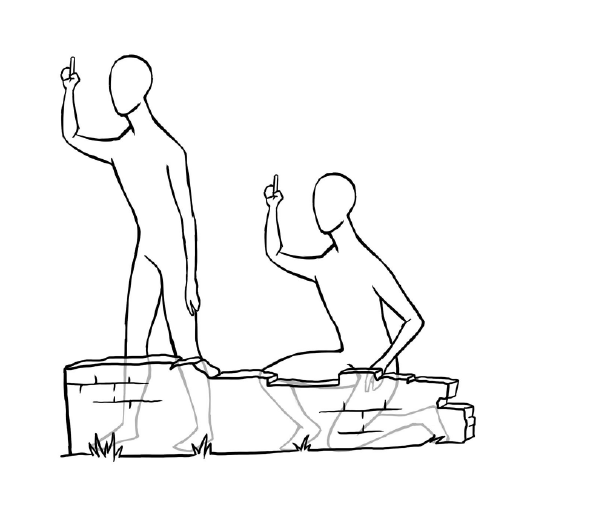
\includegraphics[width=1\textwidth]{gc-core-rules.docx.tmp/word/media/image2.png}Appendix I. Stealth Cover Diagrams

\textbf{Figure 1}: using low walls as cover for the Stealth skill. \textbf{Neither} of these people are in stealth, as the low wall does not cover at least 50\% of their size from at least one side. They would need to position themselves lower for the wall wall to provide sufficient cover.

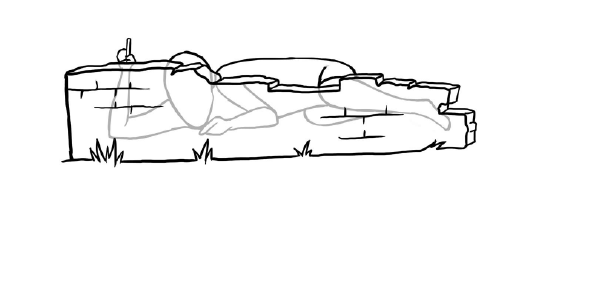
\includegraphics[width=1\textwidth]{gc-core-rules.docx.tmp/word/media/image3.png}\textbf{Figure 2}: using low walls as cover for the Stealth skill. This person is in stealth, as the low wall now covers at least 50\% of their size from at least one side.

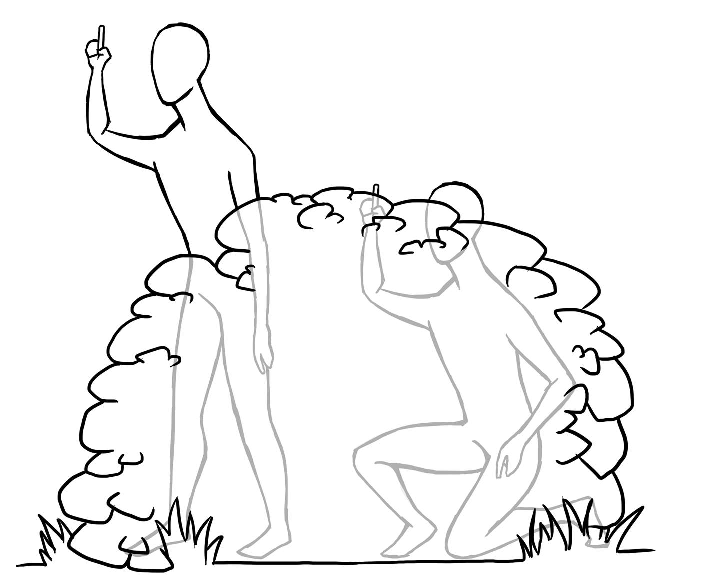
\includegraphics[width=1\textwidth]{gc-core-rules.docx.tmp/word/media/image4.png}

\textbf{Figure 3}: using bushes and mid-level undergrowth for the Stealth skill. The person on the left is \textbf{not} in stealth, as they are standing upright instead of crouched, even though the bush covers at least 50\% of their size. The figure on the right is in stealth, as they are crouching behind the bush.

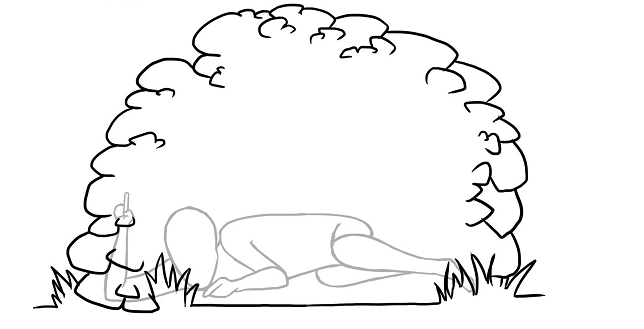
\includegraphics[width=1\textwidth]{gc-core-rules.docx.tmp/word/media/image5.png}

\textbf{Figure 4}: using bushes and mid-level undergrowth for the Stealth skill. This person is in stealth. Although just crouching would provide sufficient cover behind this bush, the person has chosen to lie down - another valid way to place yourself in stealth.

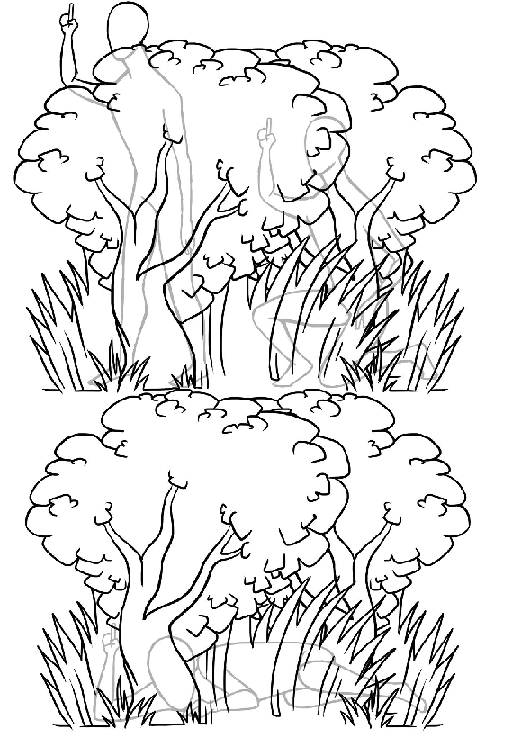
\includegraphics[width=1\textwidth]{gc-core-rules.docx.tmp/word/media/image6.png}

\textbf{Figure 5}: using trees and taller undergrowth for the Stealth skill. The person in the top left is \textbf{not} in stealth, as although the undergrowth here provides more than 50\% cover they are standing, and must be crouched or lower for it to count as stealth. The other two figures are both in stealth, as the undergrowth provides more than 50\% coverage of their size from at least one side, and they are in a crouched position or lower.

\textbf{Appendix J.} \textbf{\textit{Blastersmiths UK}} \textbf{Blaster Safety Guidelines}

\subsection{Blaster Standards}

In the interests of openness and fairness, we have laid out the standards that all blasters must adhere to, either mechanically or electrically.

Physical condition

Sharp edges and cracked plastic are not permitted: while melee striking and blocking with a blaster are banned, accidents can happen, therefore a blaster should not have sharp edges that may accidentally harm a person in this situation. Blasters that use a spring to provide power should be inspected for signs of stress if the spring has been upgraded. Particular areas of stress will be highlighted by white stress marks in the ABS plastic.

Firing capability

The blaster must be able to fire approved ammunition (see point \textit{2.2 Dart Types}) at a target. Whether or not it hits the target is irrelevant.

Muzzle velocity

The system uses a chronograph to measure the velocity (speed) of darts when they leave the muzzle of a blaster. The upper limit is 130 feet per second (39.62 metres per second). For comparison's sake, a stock (unmodified) Nerf Retaliator fires at about 65 feet per second (19.81 metres per second).

Wiring standards

The standards require that all joins are insulated with either heat shrink tubing (HST, preferred) or electrical tape. Hot glue insulation is not permitted. If a blaster has been rewired by a system-approved outfit (currently either \textit{Blastersmiths UK} or \textit{UKNerfWar}) then it passes the wiring safety standards. Otherwise, photos of the internals must be presented to the safety checker. If no such photos are available, the blaster will be opened by the player and inspected by the safety checker to ensure compliance. Blasters that are not electrical (or only have a small integrated torch, eg the Firestrike), or electrical blasters that are not modified, do not need to be opened. Evidence of intact seals may be required in order to verify modification status.

Battery standards

All batteries should be within a hard plastic case - typically the blaster's battery tray. A pack of silica gel (which absorbs moisture) is strongly recommended to ward against condensation and light rain.

\textit{AA alkalines, NiMH rechargeables and similar}

These cells should in good condition and not be leaking. In the case of NiMH, each cell should read roughly 1.2V while alkalines should read 1.5V. Often, white crusting or similar discolouration will indicate a problem with a battery. Any batteries in poor condition must be replaced in order for the blaster to be deemed safe.

\textit{TrustFire}

Extra care must be taken when handling TrustFire batteries: they are safe for use in the system but with a number of caveats. The only permitted brand of TrustFire battery is the ocial, silver-wrapped version.

Ultrareds and non-branded cells are not permitted. They must be checked after every engagement for symmetry of discharge - in other words that each battery has the same voltage. If they don't, they need to be charged. Nominal voltage should be 3.7V. Cells presenting at 3.4V or below need to be charged.

\textit{NiMH, NiCd and lithium battery Packs}

These must be checked for leakage and/or swelling. Lithium packs must have a voltage monitoring system

either a voltmeter, or an RC battery alarm. We recommend wrapping lithium packs in bubble wrap within the blaster's battery tray for extra protection against impacts. Lithium packs must read at least a voltage of 3.4V/cell (lithium polymer) or 3V/cell (lithium iron phosphate/LiFePO4).

\subsection{Ammunition Types}

Dart tip guide

Hard, dense-tipped full vinyl jacket (or ``FVJ'') darts are banned in the system. Without eye protection, these darts pose a serious risk of injury due to their dense, solid tip.

Dart types

Players are allowed to use the following dart types. There may often be a colour variant to tip types.

\textit{Off-the-shelf Hasbro darts}

\begin{itemize}
\item Orange ``streamlines'' - these are old, and no longer for sale, but are still permitted.

\item Blue ``elites'' - these are Hasbro's current ammo standard.

\item Various ``whistler'' darts - these have a large rubber head and only function in certain pistol-sized blasters. Also old, and no longer sold.

\item Various ``tagger'' darts - these have large rubber heads and velcro on their tips. Also old, hard to come by.

\item Various ``suction'' darts - Hasbro supplies two types of suction cup dart, the older Micro Suction dart and the new, blue-bodied Universal Suction Dart.

\item Various recoloured ``elite'' darts from sub-lines - eg Zombie Strike and Rebelle.

\item Mega Darts - Hasbro's newer and larger ammo type.

\end{itemize}
\textit{Aftermarket darts}

\begin{itemize}
\item ``Koosh'' darts - have a rough-looking head.

\end{itemize}
Specifically banned ammunition

Ammunition not discussed above is not permitted for use, such as Vortex (``XLR'') discs and Rebelle Arrows. All darts must be produced by an OEM manufacturer, home-made darts or modied darts are banned for use within the system. This includes, but isn't limited to, glue domes, UBER-domes and metal weighted stefans. ``Voberry'' darts / ``Voberries'' are specifically banned due to their harder heads.

Appendix K. Disclaimer

\subsection{Disclaimer}

At the site there is a variety of terrain such as woodland, fields and glades; we at \textit{Trinity Games} have done all we reasonably can to provide a safe environment for people to move in. However, due to the nature of the terrain \textit{Trinity Games} cannot be held responsible for any injuries sustained as a result of moving over the terrain. Being sensible about how people move over terrain is the sole responsibility of the individual, and by signing this form you state that you understand and agree to this at all times while you are on site. As such, \textit{Trinity Games} cannot be held accountable for any injuries sustained as a result of the terrain.

Due to the site being shared with other people in different areas, and any dangerous areas we are trying to safeguard against, any cordoned off areas are not to be entered.

On the site it is the responsibility of the individual to lift their own items, put up their own tents and transport their own kit that they have brought with them. The individual needs to judge whether they are fit/strong enough to be able to lift / manually handle any items of their own or anything else they choose to handle.

It is the responsibility of the individual to be able to judge any physical movements or lifting, and \textit{Trinity Games} cannot be held accountable for any injuries sustained as a result of improper lifting and handling of objects.

If you sustain an injury, \textit{Trinity Games} will do everything they can to help, and have risk assessments in place to try to safeguard against injuries. If you sustain an injury on site, we ask that you report it to a referee, Game Organisation Desk (GOD) or one of the team, so that a first aider can look at your injury and help where possible. If the first aider assesses that the injury needs more medical attention than has/can be given on site, you may taken to a medical facility, either by private transport or by ambulance if the first aider considers it necessary. Should this occur procedures are in place to safeguard your belongings left on-site.

It is the responsibility of the individual to make sure they are suitably nourished and hydrated while on site. Although every effort will be made to ensure running water and catering will be available on-site, there may be occasions where this is not possible, and due notice will be given in advance of events.

We often have a licensed bar on-site for adults (anyone suspected to be under the age of 18 will be asked to show identification as proof of age). If anyone is considered to be drinking excessively, having fun at the expense of other people, undertaking any illegal activity, bullying, or being too loud and/or obnoxious, then they may be spoken to by members of the team, possibly asked to leave site, and, if circumstances deem it necessary, asked not to return. \textit{Trinity Games} are here to ensure everyone has fun in a safe way. By signing this you agree to the team's decisions on any events that may cause an issue.

Anyone in a high-vis jacket bearing the \textit{Green Cloaks} logo on-site is considered to be a staff member of \textit{Trinity Games} and should be treated with respect. Sometimes they may be asked to communicate with you regarding important matters which will have been discussed by the team and passed on by them, or they may be communicating to you for your own best interest. They may also issue instructions in the case of emergency and other aspects of the game, and in this instance you are expected to follow instructions. If anyone is seen to be abusive to a member of staff they will be asked to leave the site. By signing this document you declare that you understand and agree to this.

Rules are in place to ensure safe areas, safety on site, fair play, fun and adventure. If you wish to discuss any matters with a member of the team, please send us an email at \textbf{trinitygames@hotmail.com} and we will happily discuss any issues you have concerns with.

137

Appendix L. Parent / Guardian Consent Form

If you are under the age of 18, in order to take part within games organised by \textit{Trinity Games}, this parent/

guardian consent form needs to be filled out and signed by your parent or guardian.

You, the player, must also fill out and sign the document to say that you have read the Disclaimer, that you

have understood it, and that you will adhere to its stated rules while on site.

Parent / Guardian

By signing this document you declare you have read through the Disclaimer, understand what has been said, agree to allow to your child to attend, and that they understand and agree to adhere to the rules.

\begin{table}
\begin{tabular}{|l|l|} \hline 
\textbf{Name of parent / guardian (printed)} &  \\
 \hline \textbf{Address} &  \\
 \hline \textbf{Postcode} &  \\
 \hline \textbf{Phone number} &  \\
 \hline \textbf{Signed} &  \\
 \hline \textbf{Date} &  \\
 \hline \end{tabular}

\end{table}

Emergency contact

\begin{table}
\begin{tabular}{|l|l|} \hline 
\textbf{Name} &  \\
 \hline \textbf{Relationship to player} &  \\
 \hline \textbf{Emergency contact number} &  \\
 \hline \end{tabular}

\end{table}

\textbf{Player}

By signing this document you declare you understand and agree to adhere to the rules that are in place and accept the team's judgment and decisions when made. You also agree to behave in a socially acceptable manner without issue.

\begin{table}
\begin{tabular}{|l|l|} \hline 
\textbf{Name} &  \\
 \hline \textbf{Signed} &  \\
 \hline \textbf{Date} &  \\
 \hline \end{tabular}

\end{table}

\end{document}
